%stylefile for "Progress in Particle and Nuclear Physics" from 20. March 2003
\documentclass[twoside,12pt]{article}
\usepackage{epsfig}

\def\Journal#1#2#3#4{{#1} {#2} (#4) #3 }
\def\NCA{{\em Nuovo Cimento} A}
\def\PHYS{{\em Physica}}
\def\NPA{{\em Nucl. Phys.} A}
\def\MATH{{\em J. Math. Phys.}}
\def\PRO{{\em Prog. Theor. Phys.}}
\def\NPB{{\em Nucl. Phys.} B}
\def\PLA{{\em Phys. Lett.} A}
\def\PLB{{\em Phys. Lett.} B}
\def\PLD{{\em Phys. Lett.} D}
\def\PL{{\em Phys. Lett.}}
\def\PRL{\em Phys. Rev. Lett.}
\def\PREV{\em Phys. Rev.}
\def\PREP{\em Phys. Rep.}
\def\PRA{{\em Phys. Rev.} A}
\def\PRD{{\em Phys. Rev.} D}
\def\PRC{{\em Phys. Rev.} C}
\def\PRB{{\em Phys. Rev.} B}
\def\ZPC{{\em Z. Phys.} C}
\def\ZPA{{\em Z. Phys.} A}
\def\ANNP{\em Ann. Phys. (N.Y.)}
\def\RMP{{\em Rev. Mod. Phys.}}
\def\CHEM{{\em J. Chem. Phys.}}
\def\INT{{\em Int. J. Mod. Phys.} E}
\def\r{\vec r}
\def\R{\vec R}
\def\p{\vec p}
\def\P{\vec P}
\def\q{\vec q}
\def\ss{\mbox{\boldmath $\sigma$}}
\newcommand{\be}{\begin{equation}}
\newcommand{\ee}{\end{equation}}
\newcommand{\bea}{\begin{eqnarray}}
\newcommand{\eea}{\end{eqnarray}}
\newcommand{\nn}{\nonumber}
\newcommand{\pT}{\mbox{$p_{\mathrm{T}}$}}

\topmargin-2.8cm
\oddsidemargin-1cm
\evensidemargin-1cm
\textwidth18.5cm
\textheight25.0cm
\begin{document}

\title{ \vspace{1cm} Heavy-ion collisions at the LHC}
\author{G.\ Roland,$^{1}$ K.\ \v{S}afa\v{r}\'{\i}k,$^2$ P.\ Steinberg,$^3$\\
\\
$^1$MIT, USA\\
$^2$CERN, Geneva, Switzerland\\
$^3$Brookhaven National Laboratory, Brookhaven, NY, USA\\
}
\maketitle
\begin{abstract} 
A new era in the study of high-energy nuclear collisions began when the 
CERN Large Hadron Collider (LHC) provided the first collisions of lead nuclei
in late 2010. In the first three years of operation the ALICE, ATLAS and CMS 
experiments each collected \PbPb\ data samples of more than 150\mubinv at 
$\rootsNN = 2.76$\TeV, exceeding the previously studied collision energies 
by more than an order of magnitude. These data provided new insights into
the properties of QCD matter under extreme conditions, with extensive
measurements of soft particle production and newly accessible probes
of hard probes of the hot and dense medium. In this reviwe, we provide
a comprehensive overview of the results obtained in heavy-ion collisions
at the LHC so far, with particular emphasis on the complementary nature
of the observations by the three experiments.
\end{abstract}

%\eject
%\tableofcontents
\section{Introduction}
\label{secall:intro}
The first ideas about heavy-ion experiments at the Large Hadron Collider (LHC)~\cite{Evans:2008zzb} at CERN were formed in the early nineties (in the last century)~\cite{Jarlskog:1990dv}. Since the beginning of the LHC project, approved by CERN Council in 1994, the investigation of heavy-ion collisions was an integral part of the LHC physics programme. Built from 1998 to 2008 in the 27~km long (approximately) circular underground tunnel, exploited before by the Large Electron--Positron (LEP) collider, the LHC machine represents the highest-energy particle accelerator ever made. This very versatile collider is designed to reach centre-of-mass energies up to $\sqrt{s} = 14$~TeV for proton--proton (pp) collisions, and up to 1\,150~TeV using lead-ion beams, corresponding to $\sqrt{s_{\rm NN}} = 5.5$~TeV per colliding nucleon pair. These will entail the energy increase by a factor of seven for hadron collisions, and and more than 27 for heavy-ion collisions compared to predecessor colliders.
\subsection{Physics motivation}
\label{subsecall:motivation}
At very high temperatures and densities, hadronic matter is expected to undergo a phase transition into a qualitatively different state, where quark and gluon degrees of freedom are liberated. Such conditions were prevailing in the early Universe, a few microseconds after its formation. In heavy-ion collisions at ultra-relativistic energies, nuclear matter is heated and compressed reaching conditions well beyond the phase-transition point, and the same type of medium filling the very early Universe is thus momentarily re-created. At the highest available energies, at the LHC, far better conditions, than those at the other existing facilities, are achieved to study this new state of matter, called the Quark--Gluon Plasma (QGP). The nearly-vanishing baryon density, the highest available initial temperature and energy density, and the abundance of perturbatively-calculable hard Quantum Chromo-Dynamics (QCD) processes make heavy-ion collisions at the LHC particularly well-suited for precision studies of the QGP properties.

QCD, the well-established theory of strong interactions, predicts (cross-over) phase transitions in strongly interacting matter at high temperatures. A phase transition reflects breaking of a fundamental symmetry in the theory. Above the critical temperature, ordinary hadronic matter, where protons and neutrons are composed of quarks and gluons confined in a colour-neutral state, melts during the deconfinement phase transition. In the deconfined medium, quarks and gluons are not bound into hadrons anymore, however, the effective degrees of freedom of the QGP, formed at temperatures achieved with heavy-ion collisions, are rather complex. A second phase transition is connected with the generation of hadron masses as a consequence of the presence of a quark--antiquark condensate in the vacuum at low temperature. According to QCD, at high temperatures, the vacuum condensate is reduced, and the masses of quarks drop to their bare values during a chiral phase transition. Quantitative lattice QCD calculations~\cite{Borsanyi:2010bp} confirm that QCD matter undergoes a transition from a hadronic gas to a QGP at a temperature about 160~MeV, corresponding to an energy density of about 0.5~GeV/fm$^3$. At LHC conditions (small baryon density), the transition is a smooth cross-over spanning a temperature range of 20--30~MeV, which means that the precise value of the critical temperature depends on the observable used to locate it.

In a heavy-ion collision the energy deposited at the mid-rapidity is determined by the density of low-$x$ (Bjorken $x$, corresponds approximately to the fraction of nucleon longitudinal momentum carried by a parton) gluons confined in the colliding nuclei. The relevant values of $x$ at LHC energies are order of magnitude smaller than those at RHIC, i.e. on the $10^{-3}$ level and below. In such small-$x$ range, at low virtualities the perturbative gluon distribution reaches the saturation and gluons have to fuse, in order not to violate unitarity.  This marks the transition to the non-linear parton-evolution region, and the virtuality scale at which this transition happens is known as the saturation scale $Q_{\rm s}$. It increases (logarithmically) with the incident energy, and the mass of colliding nuclei (as nucleon radius), and  reaches the values $Q_{\rm s} \approx 3$--$4$~GeV$^2$ for Pb--Pb collisions at the LHC. During the collision of the two nuclei, these dense gluon fields are deconfined and create a primordial strongly-interacting medium, which rapidly expands and thermalizes. The thermalized QGP continues to cool down, mainly by the longitudinal expansion, until its temperature decreases below the critical temperature of the QCD phase transitions, and then it is converted into a gas of hadron resonances. At this moment the produced-particle composition is frozen, and the corresponding temperature is called the chemical freeze-out temperature ($T_{\rm ch}$), presumably being close to the critical temperature of the QCD phase transitions. Hadrons still continue to interact, however, as their relative energy is below the threshold for inelastic production, only their momentum spectra are modified. At a kinetic freeze-out, with corresponding kinetic freeze-out temperature ($T_{\rm kin}$), the medium is diluted that the final hadrons decouple, ceasing any interaction with the rest.

Prior to the start-up of the LHC heavy-ion programme, the nature of the QGP as an almost-perfect, inviscid liquid emerged from the experimental investigations at RHIC~\cite{Tribble:2007nsac}. The pressure created in the thermalized QGP phase is reflected in the large azimuthal asymmetry observed in the final-state particle production. The resistance of the medium  to the shape change implies a very low shear viscosity, or in dimensionless variable, a very low ratio of shear-viscosity to entropy-density in the QGP. Consequently, it evidences extremely short mean-free path inside the medium at this stage of the evolution (and the corresponding cross section approaching the unitarity limit) induced by a complex excitation modes in strongly-coupled QCD medium. This also implies the development of the collective transverse velocity field at this stage, which contributes to the plasma cooling. The smallness of the mean-free path with respect to the system size allows for the successful utilization of relativistic hydrodynamics in the description of the evolution of the thermalized QGP until hadronization.

Such an interpretation is further supported by the observation of the strong energy loss of partons traversing this strongly-coupled QCD medium, demonstrated at RHIC with large suppression of particle production at transverse momenta ($p_{\rm T}$) up to 20~GeV. Deduced from these measurements, the large amount of the energy loosed by hard partons due to the gluon bremsstrahlung and by elastic collisions is consistent with the low shear viscosity established from the collective-flow pattern of low-momentum hadrons. With the first LHC data, this basic picture is confirmed, observing the creation of deconfined matter at unprecedented values of temperatures, densities and volumes~\cite{Muller:2012zq}. The origin of this almost-perfect-fluid QGP behaviour  is the subject of further experimental study at the LHC. Among the interesting interrogations to answer are: if the predicted initial gluon saturation reduces also the low-$p_{\rm T}$ particle yields; and if the low shear viscosity is affected by the expected increase of the QGP temperature at an early stage. However, the most important impact of the more than order of magnitude increase of the collision energy is the much higher rates for hard probes, such as the jets, electro-weak particles, heavy flavours, and quarkonia. The high rates allow for precision studies of the QGP using the in-medium interactions of these probes, better controlled theoretically than the propagation of light partons. In addition, some observables, e.g. very high-energy jets, electro-weak bosons, and different $\Upsilon$ states, are accessible in heavy-ion collisions for the first time. A comprehensive compilation of theoretical predictions for the LHC heavy-ion programme was published in~\cite{Abreu:2007kv}.
 
The experimental results obtained using heavy-ion collisions during the first period of the LHC running are summarized in this article. It is divided into the sections according to various heavy-ion observables: Sec.~\ref{secks:eventchar} describes the principals of centrality selection and measurements of particle and energy densities; particle yields and spectra are discussed in Sec.~\ref{secks:spectra}; correlation studies are explicated in Sec.~\ref{secks:nonflow} for non-flow effects, and in Sec.~\ref{sec:ps:flow} for flow phenomena; Sec.~\ref{sect:pas:ew} deals with production of electro-weak particles; Sec.~\ref{jets_intro} is dedicated to jets and their quenching; and to heavy flavours two sections are devoted, Sec.~\ref{secks:heavy} to open heavy flavours, and Sec.~\ref{} to quarkonia. Summary and outlook are given in Sec.~\ref{secall:summary}.

\subsection{LHC heavy-ion running}
\label{subsecall:running}

\begin{figure}[!htb]
\begin{center}
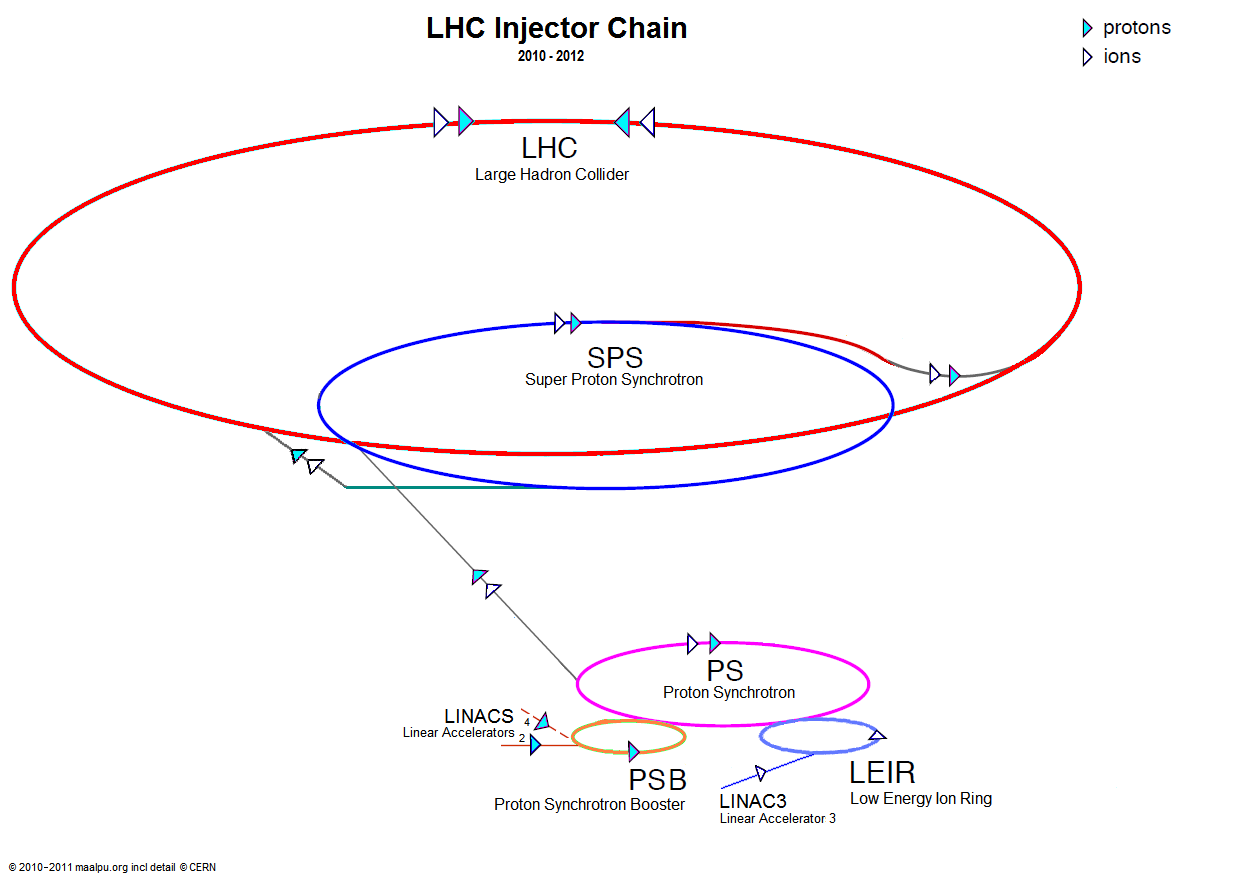
\includegraphics[width=0.8\textwidth]{introduction_figs/LHC_chain.png}
\caption[]{Schematic view of LHC injector chain, showing the path of both protons and ions.}
\label{fig:pas:intro:lhc}
\end{center}
\end{figure}

Heavy ion running at the Large Hadron Collider had been planned long before the machine was built.
This was based on the interest in the physics at the CERN SPS, which was colliding light ions since
1986 and heavy ions since 1994, and as a natural extension to the already-planned program
at the Relativistic Heavy Ion Collider (RHIC).
The accelerator complex is shown in Figure~\ref{fig:pas:intro:lhc}.
Ions start their path to collisions at the ECR (electron cyclotron resonance) ion source,
which provides lead ions stripped to values around Pb$^{29+}$, which are passed through
a spectrometer to select Pb$^{29+}$ and accelerated in a linear accelerator to 4.2 MeV/n.
They are then stripped to around Pb$^{54+}$ by a 0.3 $\mu$m carbon foil and the
Pb$^{54+}$ are selected by a spectrometer to be fed into the CERN Low Energy Ion Ring (LEIR).
LEIR is used to transform a set of low intensity ion pulses from the LINAC into shorter
bunches with higher intensity.  This is done by filling the available phase space in
three dimensions.  After this, electron cooling is applied to shrink the beam to increase the
bunch density, and decelerate it into ``a stack sitting slightly inside the central orbit''.
At this point, seven pulses are captured, split into two bunches, and then accelerated to
72 MeV/n.
The bunches from LEIR are then sent to the CERN PS (Proton Synchrotron), accelerated to
5.9 GeV/n and stripped fully to Pb$^{82+}$ using a 0.8 mm aluminium foil.  These ions
are then sent to the SPS where they are acceleated to 177 GeV/n and injected into the LHC.

To date, there have been three heavy ion runs at the LHC.
The first run was in November/December 2010,
which provided 120 colliding bunches of lead ions in each ring, with a center of mass energy per nucleon
pair of $\energy =2.76$ TeV, a peak luminosity of $3 \times 10^{25} / \mathrm{cm}^2 s$ and an integrated luminosity
of 7 $\mu \mathrm{b}^{-1}$, corresponding to about 50 million minimum bias events.
The second run was in November/December 2011, which provided about 360 colliding bunches of lead ions per ring,
also at $\energy =2.76$ TeV, a peak luminosity of
about $5 \times 10^{26}  / \mathrm{cm}^2 s$ and an integrated luminosity of
about 150 $\mu \mathrm{b}^{-1}$, a factor of 20 increase over 2010.
The third run, in January/February 2013, provided proton-lead collisions
at $\energy=5.02$ TeV but these results are not discussed
in detail in this review.

\subsection{Detectors at the LHC}
\label{subsecall:detectors}

Three, out of the four principal LHC detectors, participate in the LHC heavy-ion programme. These are: ALICE (A Large Ion Collider Experiment), a dedicated heavy-ion detector designed to operate in the high particle density environment; and two general-purpose particle detectors, ATLAS (... Toroidal ... whatever) and the CMS (Compact Muon Spectrometer), optimized to high interaction rates and capable of precision measurements at very high transverse momenta. The fourth detector, the LHCb, was not taking data in Pb--Pb runs due to the occupancy limitation, however, it participated in the p--Pb run, and reported interesting results. 

\subsubsection{ALICE}

\begin{figure}
\begin{center}
\includegraphics[height=0.49\textwidth]{introduction_figs/ALICEdet.png}
\caption{Schematic layout of the ALICE detector, indicating the main subsystems. The inset in top-right corner shows the innermost part in detail.}
\label{figks:ALICEdet}
\end{center}
\end{figure}


The ALICE detector~\cite{Aamodt:2008zz} is shown in Fig.~\ref{figks:ALICEdet}, and it has the following main parts: central barrel, muon arm, and forward detectors. The central barrel is housed in a large solenoid magnet providing the field of 0.5~T, with 12~m aperture and 12~m length, which was inherited from the L3 experiment running at the LEP collider. This part provides measurements of particles produced within about $\pm 45^\circ$ with respect to a plane perpendicular to the beam axis, corresponding to pseudorapidity coverage $|\eta| < 0.9$ ($\eta = - \ln \tan (\Theta/2)$, where $\Theta$ is the angle from the beam axis). The six-layer silicon Inner Tracking System (ITS), surrounding the beryllium vacuum beam pipe 6~cm in diameter, begins with pixel detectors at radii 4 and 8~cm, continues with silicon-drift detectors at 14 and 22~cm, and ends with double-sided strip detectors at 39 and 43~cm. The ITS measures the particle tracks with position precision of a few tens of microns. In addition, the four outer layers participate in the Particle Identification (PID) by determining the specific ionization energy loss (${\rm d}E/{\rm d}x$). The excellent spatial resolution of the innermost silicon pixel layers results in outstanding capabilities of primary and secondary vertex reconstruction.  The resolution in measuring the distance of closest approach to the primary vertex for tracks coming from secondary decays is for transverse momentum \pT of 1~GeV between 60--70~$\mu$m, allowing to detect weak decays of charm and beauty particles.
The main particle tracking device is the TPC (Time Projection Chamber), the largest such detector built to now. It has a cylindrical shape, more than 5~m along the beam axis, and 5~m in outer diameter. The TPC continues the tracking from the ITS at a radius of 88~cm and carries on till the end of its sensitive volume. The TPC volume, filled with neon-based gas mixture, is divided into two halves by a thin central high-voltage electrode providing an electrostatic field of about 0.4~kV/cm. Electrons created by ionization in the gas drift towards one of the end-plates equipped with multi-wire proportional chambers with cathode-pad readout. Altogether the TPC is read out with more than 600~thousands pads, which gives, taking into account the sampling along the drift direction, an effective granularity in the TPC volume of more than half a billion three-dimensional pixels. Consequently, this results in very efficient track-finding down to low transverse momenta, about 100~MeV, even at the highest particle densities in central lead--lead collisions at LHC energies. In addition, the ALICE TPC has an excellent resolution for the measurement of ${\rm d}E/{\rm d}x$, between 5 and 6\,\%, depending on particle density. 
The momentum dependencies of ${\rm d}E/{\rm d}x$ for different particles cross when approaching their minima for ionization energy losses. This makes particle identification using such method impossible in that momentum region. To distinguish particle species in this region, ALICE installed a Time-Of-Flight detector (TOF) at a radius of about 3.7~m from the beam axis. This detector determines the arrival time of charged particles with a precision better than 100~ps, exploiting multi-gap resistive plate chambers, an innovative technology developed specifically for ALICE. The TOF measurement is able to separate pions and kaons up to 2.2~GeV, K mesons and protons up to 3.5~GeV, and can be used for electron identification at lower momenta. To further increase the momentum reach for charged hadron identification, a smaller detector, the High-Momentum PID (HMPID), covering about 10\,\% of to the other central barrel detectors and using \v{C}erenkov ring-imaging technique, is placed at a distance of 1~m larger than that of TOF. To improve the electron identification ALICE uses a Transition Radiation Detector (TRD) situated between the TPC and TOF detectors. Particles traverse six radial drift chambers, each consisting of a transition radiator followed be a volume containing a xenon-based gas mixture, allowing the detection of X-ray photons in addition to charged tracks. The TRD drift chambers are read out with cathode-pad wire chambers. Electrons are separated from pions by discriminating on signal amplitude of last samples, where the electron transition radiation contributes. This detector is also used in the tracking system; an increase of the track length in magnetic field improves the momentum resolution at high transverse momenta (to about 5\,\% around 100~GeV). At low momenta, 0.1--1~GeV, the momentum resolution of ALICE tracking system is better than 1\,\%. The central barrel part of ALICE is completed with electromagnetic calorimeters. The larger one, EMCal, covers $120^\circ$ in azimuthal angle and in longitudinal direction a little less than the barrel detectors in front of it. It is used to trigger on jets and to improve the jet energy determination measured with tracking detectors. The much smaller Photon Spectrometer (PHOS) has significantly better energy resolution and granularity, and is dedicated to the isolation of a direct photon signal in heavy-ion collisions.

The ALICE detector can detect and trigger on muons in the forward region on one side of the central barrel using its muon arm, between $2^\circ$ and $9^\circ$ from the beam axis. A conical absorber begins at only 90~cm from the nominal interaction point, in order to suppress the background from decaying pions and kaons. Behind the absorber, the five tracking stations detect the filtered out muons. The first two stations are still inside the main solenoid magnet; the third one is in the middle of the ancillary dipole magnet with 3~Tm of field integral used for muon momentum analysis; the remaining two measure deflected muon tracks behind the dipole. Each tracking station consists of two planes of multi-wire chambers with cathode-pad readout, giving a coordinate precision of about 100~$\mu$m in the bending plane, thus giving a mass resolution of 1\,\% at the $\Upsilon$ mass, needed for the separation of different $\Upsilon$ states. Behind the last muon tracking station a second absorber shields the muon trigger detectors from remaining background. The full length of the muon arm, from the interaction point to the end of the trigger system, is about 20~m. Two trigger planes of Resistive Plane Chambers (RPC) detect the position and direction of penetrating muons. Using this information the muon trigger electronics select events having muons with transverse momentum above a predetermined threshold.

On the side opposite to the muon arm the Photon Multiplicity Detector (PMD) measures the yield of $\pi^0$ mesons by counting the number of photons. The Forward Multiplicity Detector (FMD), with silicon strip planes on both sides of the interaction region, determines the density of charged particles emitted at pseudorapidities $-3.4 < \eta -1.7$ and $1.7 < \eta < 5$. Scintallator tile arrays (called VZERO), covering similar acceptance to the FMD, are used to trigger on LHC collisions, in heavy-ion collisions also selecting different centrality classes with corresponding thresholds. Small quartz counters on both sides (T0 detector) are employed in time-of-flight measurements. The Zero Degree Calorimeters (ZDC) are placed more than 100~m from the interaction region in both directions; on each side there is one for the detection of proton spectators and second for neutron spectators.



\subsubsection{ATLAS}

\begin{figure}[!htb]
\begin{center}
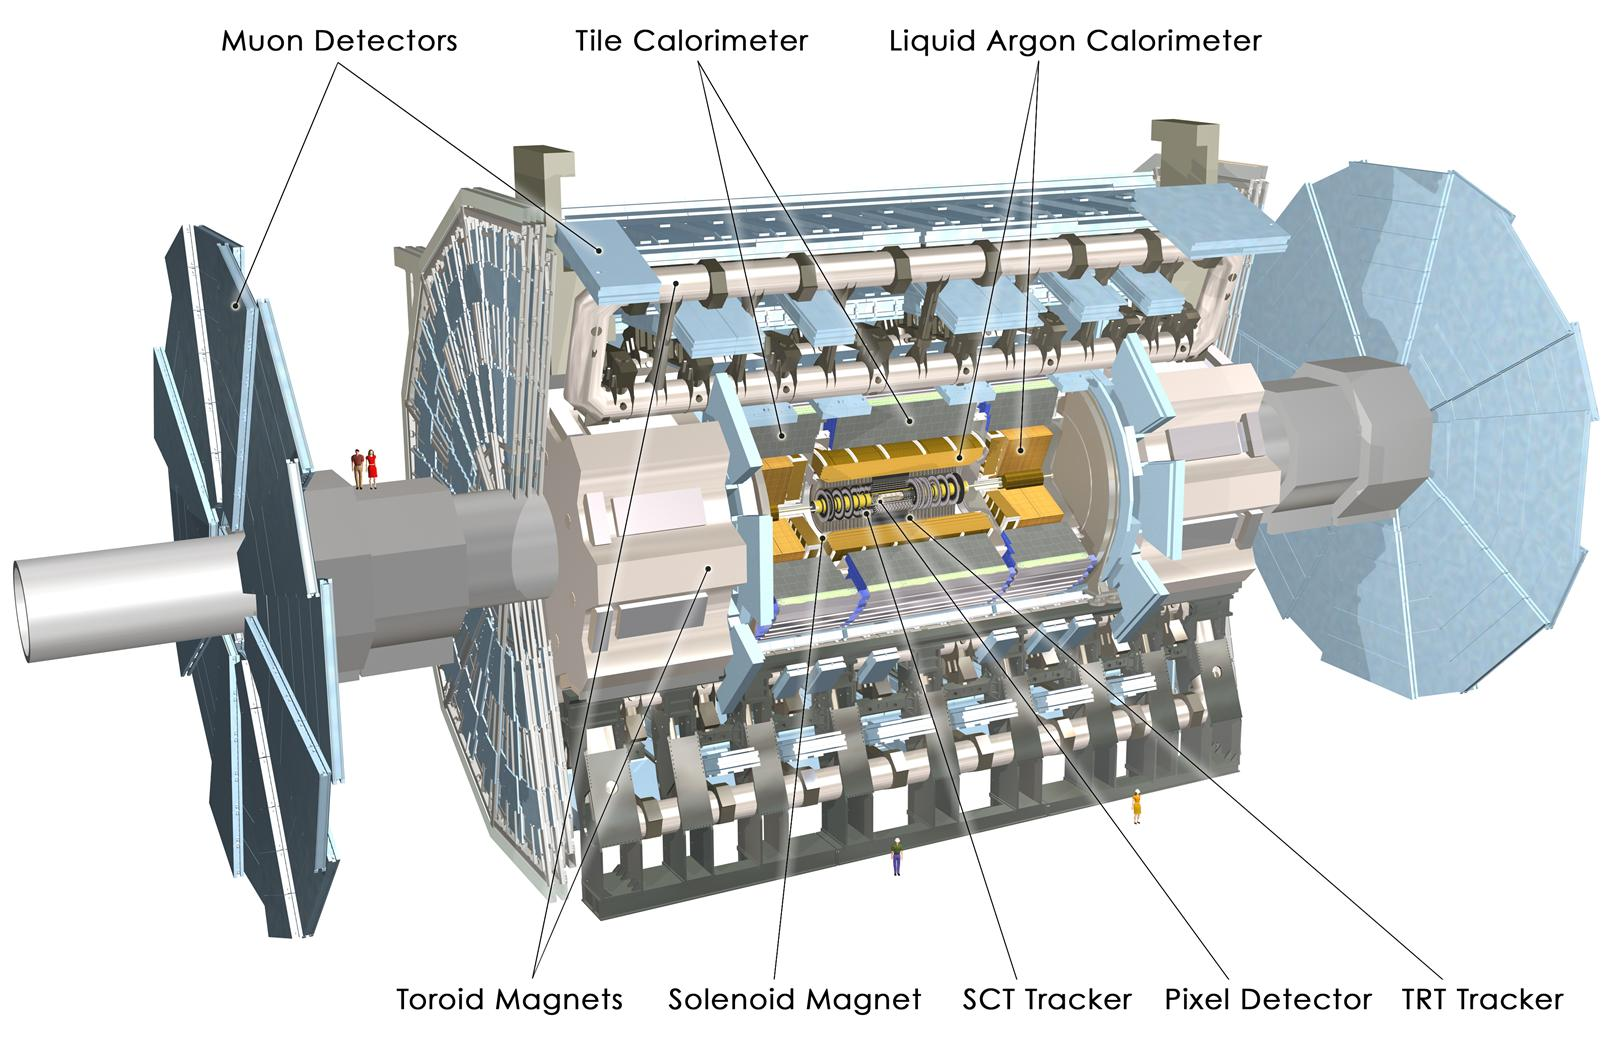
\includegraphics[height=0.49\textwidth]{introduction_figs/0803012_05-A4-at-144-dpi.jpg}
\caption[]{Schematic view of ATLAS detector at the LHC, highlighting the major subsystems.}
\label{fig:pas:intro:atlas}
\end{center}
\end{figure}

%ATLAS
The ATLAS detector~\cite{Aad:2008zzm}, shown in Figure~\ref{fig:pas:intro:atlas} is one of the general-purpose particle physics
detectors at the LHC.
It has three main detector systems: the inner detector (ID), the calorimeter,
and the muon spectrometer (MS).
%
The inner detector tracks charged particles using three separate detector
technologies, and the spectrometer is immersed in a 2T axial field from a
superconducting solenoid magnet 1.2m from the nominal beam axis.
The pixel detector typically provides three high-resolution space points
with three layers of pixel detector surrounding the beam pipe within
$|z|<400 mm$ (covering approximately $|\eta|<2$ and 4 disks at forward
angles covering out to $|\eta|<2.5$.
The semiconductor tracker detectors are silicon strips covering out to
$|\eta|<X$ in the barrel region and $|\eta|<2.5$ in the forward regions.
The transition-radiation tracker covers $|\eta|<2$ with straw tubes in
both the barrel and forward regions.
%
The ATLAS calorimeter has large coverage in pseudorapidity ($|\eta|<4.9$)
and longitudinal segmentation in both electromagnetic and hadronic
sections.
In the barrel region, the electromagnetic calorimeter has three
layers and a presampler layer, all using liquid argon technology.
The first layer has very high resolution
in the $\eta$ direction, allowing discrimination of photons from
neutral hadron decays.
The second layer is coarser but deeper, providing the primary energy
measurement for electromagnetically interacting particles (photons and
electrons), while the third layer is there to catch the tails of the
deposited electromagnetic showers.
%
The ATLAS hadronic calorimeter uses steel absorber and measures the
hadronic showers by means of scintillating tiles.
In the endcap region, beyond $|\eta|=2$,
both hadronic and electromagnetic sections use LAr technology with
relativly coarse cell segmentation.
The ATLAS forward calorimeter (FCal) covers $|\eta|=3.2-4.9$, using
a matrix of copper and liquid argon in the electromagnetic section,
and tungsten and liquid argon for the hadronic section.
%
The ATLAS muon spectrometer covers $|\eta|<2.7$ with precision drift
chambers
in the barrel region and cathode strip chambers in the forward region.
The bending of muons is provided by three air-core toroids, giving
a momentum resolution ranging from approximately 2\% up to about
10\% at $\pT=1$ TeV.
%

ATLAS provides a sophisticated multi-level trigger system for
selection of physics objects (jets, taus, photons, electrons, muons,
and missing transverse energy).
Jet triggering is done both seeding on energy deposited into localized
regions of the calorimeter, as well as a full reconstruction of the jets
using a similar algorithm as used in the offline analysis.
Electron and photon triggering uses smaller regions in the calorimeter
than for jets, and also applies selections based on the measured shower
shape and leakage in the hadronic sections.
Muon triggering is provided by thin-gap chambers and resistive plate chambers,
covering about 90\% of the solid angle out to $|\eta|=2.7$.
In general, triggering on tau leptons and missing transverse energy (e.g.
from $W$ bosons) is not utilized for any heavy ion analysis, as both
are highly contaminated by the large fluctuations in the
underlying event.

\subsubsection{CMS}

\begin{figure}
\begin{center}
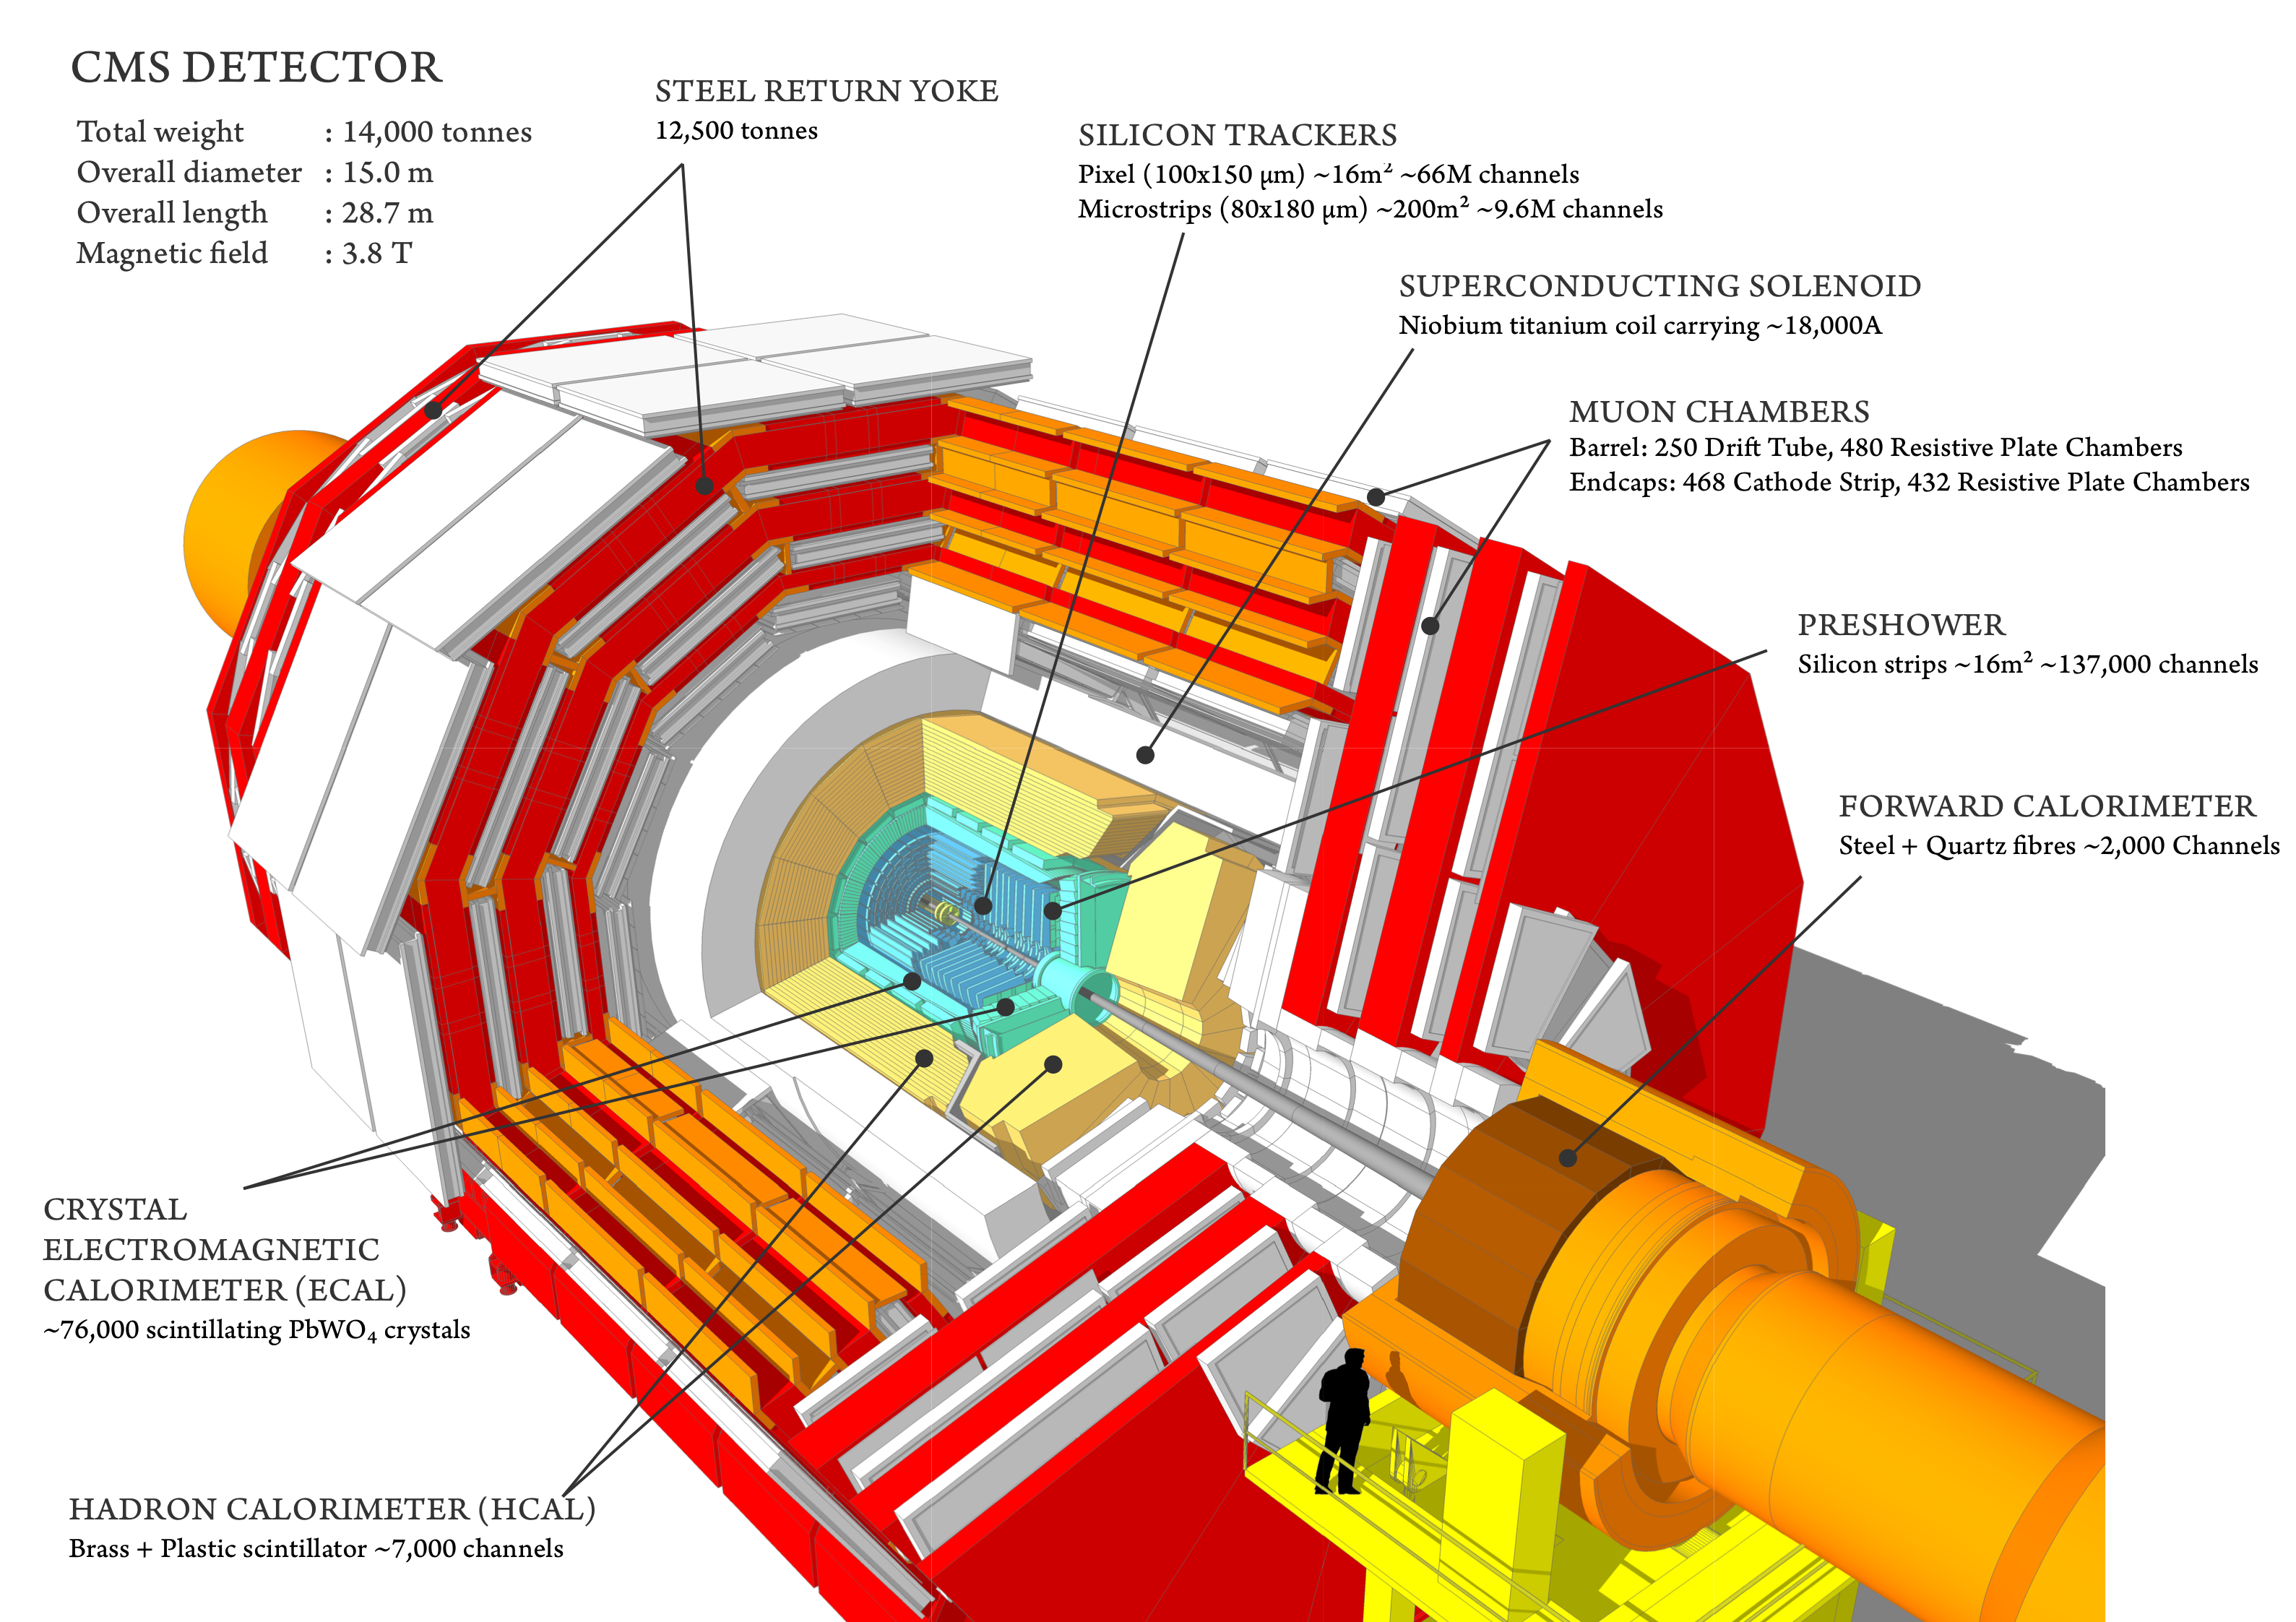
\includegraphics[height=0.49\textwidth]{introduction_figs/cms_120918_03.png}
\caption{Schematic layout of the CMS detector showing its main subsystems.}
\label{ntroduction_figs:CMSdet}
\end{center}
\end{figure}
The Compact Muon Solenoid (CMS) is a general purpose collider detector at the LHC. A detailed description of the CMS experiment
can be found in~\cite{Chatrchyan:2008zzk}. 
As shown in Fig.~\ref{CMSdet},  the apparatus has an overall length of 22~m, a diameter of 15~m, and weighs 14\,000~tonnes.
The central feature of the experiment is a superconducting solenoid
of 6~m diameter. The large magnetic field of 3.8~T provided by the solenoid is essential for achieving
the very high momentum resolution that is one of the strength's of the experiment.
Within the volume of the magnet are a silicon pixel and strip tracker, a lead tungstate crystal
electromagnetic calorimeter (ECAL), and a brass/scintillator hadron calorimeter (HCAL).
The silicon tracker measures charged particles in $|\eta|< 2.5$.
For 100\GeVc\ particles, an impact parameter resolution of $\approx 15\mu$m and a \pt\
resolution of about 1.5\% for 100\GeV [100\GeVc] particles are achieved.
The ECAL consists of 75\,848 lead tungstate crystals covering $|\eta|< 1.479 $ in the
barrel region (EB) and $1.479 < |\eta| < 3.0$ in two endcap regions (EE).
A two-plane lead/silicon preshower detector is located  in front of the EE.
The photon energy resolution of the ECAL at  $E_{\rm T} {\approx} 60$\GeV ranges from
 1.1\% and 2.6\% in the EB region and from and from 2.2\% to 5\% in the
endcaps. 
Using the particle flow algorithm, which combines information from the inner tracker
and calorimeters, the jet energy resolution achieved in \pp\ collisions typically
is 15\% at 10\GeV, 8\% at 100\GeV, and 4\% at 1\TeV, 
which compares to about 40\%, 12\%, and 5\% obtained when the calorimeters alone 
are used for jet finding.
Forward calorimeters extend the rapidity coverage provided by barrel and endcap detectors.

In the steel return yoke outside the magnet, detectors are embedded for muon identification.
The muon detectors cover $|\eta|< 2.4$ using three detector technologies:
drift tubes, cathode strip chambers, and resistive plate chambers.
Matching muons to tracks in the silicon tracker allows a \pt\ resolution between
1 and 5\%, for \pt values up to 1\TeV.

The detector operates in identical configuration for \pp\ and \PbPb\ data taking.
The main operational difference is the configuration of the two-stage trigger system.
The first level (L1) of the trigger system employs custom hardware processors
and  uses information from the calorimeters and muon detectors to select the most
interesting events in a fixed time interval of less than 4$\mu$s.
The High Level Trigger (HLT) processor farm, based on commodity hardware,
decreases the event rate to several 100~Hz for final data storage.
For heavy-ion data taking, custom reconstruction algorithms  executed in
the HLT permit the selection of events based on photon, muon, jet and
single-track signatures, in connection with global event properties such
as charged track multiplicity or energy deposited in the calorimeters.

\section{Event characterization}
\label{secks:eventchar}

The first analyses of LHC heavy-ion data dealt with the charged particle density and the energy density achieved in Pb--Pb interactions at an unprecedent collision energy of $\sqrt{s_{\rm NN}} = 2.76$~TeV per nucleon pair in centre-of-mass system. The estimated values, as well as the results of practically all other measurements, strongly depend on the geometry of the collision, also called centrality.
%more precisely on the distance $b$ of the centres of colliding nuclei in the plane transverse to the beam axis, called impact parameter of the collision.
%The impact parameter determines the volume of the interaction region, i.e. how violent the collision was.
%how many nucleons from the incoming nuclei actually took part in the collision
In this section we first describe how the centrality of Pb--Pb collisions is determined, and then we turn to the basic measurements which characterize these interactions at the LHC.



\subsection{Centrality determination}
\label{subsecks:centrality}

The lead nuclei are relatively extended objects, their size is about 14~fm across. To classify events according what part of the two nuclei participated in the interaction, the concept of collision centrality is commonly introduced in the field of heavy-ion physics. The centrality of the collision can be expressed in terms of geometrical parameters, such as the impact parameter $b$  (the distance of the centres of colliding nuclei in the plane transverse to the beam axis), or the number of participating nucleons $N_{\rm part}$ (the number of nucleons from the incoming nuclei actually taking part in the collision). These parameters are inferred by comparison of experimental data with simulations of interactions. In this context the geometrical Glauber model is typically used~\cite{Miller:2007ri}, based on a description of pA and A--A scattering, originally proposed by R.J.~Glauber~\cite{Glauber:1955qq,Glauber:2006gd}. For the event simulation a Monte Carlo implementation of Glauber model is exploited~\cite{Shor:1988vk,Alver:2008aq}, which is realized by the following steps:
\begin{itemize}
    \item{randomly sample the position of each nucleon inside the nucleus according to a Woods--Saxon distribution (two-parameter Fermi distribution), optionally taking into account a nucleon-exclusion volume (hard-core potential), and using the parameters extracted from the analysis of low-energy elastic e--A scattering~\cite{DeJager:1987qc};}
    \item{randomly sample the collision impact parameter $b$ with probability distribution $P(b) \propto b \, {\rm d}b$ (up to $b_{\rm max} = 20$~fm, i.e. well above the lead nucleus diameter);}
    \item{assuming nucleons are moving along straight lines parallel to the beam direction, a pair of nucleons is considered as colliding if their centres are closer than $\sqrt{\sigma_{\rm NN}/\pi}$ in the transverse plane, where $\sigma_{\rm NN} = (64 \pm 5)$~mb is the inelastic nucleon--nucleon cross section, estimated from LHC pp measurements;}
\end{itemize}
and for each event the number of nucleons participating in at least one collision ($N_{\rm part}$) and the number of these binary collisions ($N_{\rm coll}$) are counted. Then the total nuclear Pb--Pb cross section ($\sigma_{\rm PbPb}$) is calculated as the fraction of $\pi b_{\rm max}^2$ given by the ratio of the number of events with $N_{\rm coll} \geq 1$ to the number of all generated events. The cross section for collisions with impact parameter in the interval $(0, b)$ is obtained the same way, counting the events with $N_{\rm coll} \geq 1$ having the impact parameter within that interval. The centrality for this impact-parameter selection is its cross section expressed as the percentage of $\sigma_{\rm PbPb}$. A centrality class is defined by its lower and upper percentages, corresponding to the events within impact-parameter interval $(b_{\rm l}, b_{\rm u})$, where the lower percentage is the part of $\sigma_{\rm PbPb}$ up to the impact parameter $b_{\rm l}$ and the upper percentage is that part up to $b_{\rm u}$. Other characterizations of centrality classes, such as the mean number of participants $\langle N_{\rm part} \rangle$ and the mean number of binary collisions $\langle N_{\rm coll} \rangle$ (obtained as the average values for events within that class) are also employed. For completeness, the geometrical overlap function (integral of the convolution  of the two transverse nuclear densities in the overlapping region) in the Monte Carlo formulation of Glauber model is defined as $T_{\rm AA} = N_{\rm coll} / \sigma_{\rm NN}$.

However, none of the geometrical quantities mentioned above ($b$, $N_{\rm part}$, $N_{\rm coll}$) is directly measurable in an experiment. Therefore, an experimental observable, which strongly correlates with the collision impact parameter, has to be used to classify the events according to their centrality. For example, the charged-particle multiplicity $N_{\rm ch}$ (or the energy deposition in a calorimeter) within a given pseudorapidity region is often used. In what follows the centrality determination as implemented by the ALICE collaboration is described~\cite{Abelev:2013qoq}, and later the differences for other experiments are mentioned. The centrality selection of events within a certain impact-parameter interval is then replaced by a selection using a $N_{\rm ch}$ interval. In an ideal case, if one were able to measure the event distribution in such new selection variable for all Pb--Pb nuclear collisions, it would be possible to define centrality selection and centrality percentiles without any model, using only this distribution and its integral. However, for very peripheral collisions (large $b$, low $N_{\rm ch}$) the experimental event sample is contaminated by electromagnetic interactions, at LHC energies these processes have  a huge cross section (more than two orders of magnitude larger than the nuclear cross section) and contribute to low multiplicity events~\cite{Bruce:2009bg,ALICE:2012aa}. It is necessary to suppress them, at least partly, already during the data taking (triggering on a minimum multiplicity value, or requiring some signal in ZDC's, see Sec.~\ref{subsecall:detectors}), which inevitably makes the event trigger less efficient for very peripheral collisions. For these reasons, the event distribution in a variable such as $N_{\rm ch}$ is usable for centrality selection only above some value, typically excluding peripheral collisions corresponding to the centrality class 90--100\,\%, where the contamination and the trigger inefficiency cannot be neglected. In order to determine the value, from which the distribution can be used, and to relate this so-called anchor point to the centrality, two approaches are utilized. The simulation of the Pb--Pb electromagnetic processes together with the experiment's trigger response gives the possibility to correct the event distribution of the selection variable, and to estimate a reasonable position of the anchor point with its centrality. Alternatively, the Glauber Monte Carlo can be supplemented with a model of particle production, describing the experimental selection-variable distribution and finding the point where the two deviate. Such an approach also allows to calculate for a given centrality selection the corresponding $\langle N_{\rm part} \rangle$ and $\langle N_{\rm coll} \rangle$, taking into account the finite resolution of the selection variable $N_{\rm ch}$ with respect to the collision impact parameter $b$.

A simple model for multiplicity production, exploited together with a Glauber Monte Carlo, consists in the simulation of the multiplicity distribution from one particle source and a prescription for the number of particle sources depending on the collision geometry, called the number of ancestors ($N_{\rm anc}$). For the multiplicity distribution the Negative Binomial Distribution (NBD) is typically used, it has two parameters (controlling the mean and width), and describes reasonably well the charged-particle multiplicity in different pseudorapidity windows for high-energy pp interactions. The number of particle sources is parameterized as a function of $N_{\rm part}$ and $N_{\rm coll}$, the common choice being $N_{\rm anc} = f N_{\rm part} + (1 - f) N_{\rm coll}$, motivated by a two-component model, where the number of sources is composed of soft (proportional to $N_{\rm part}$) and hard (proportional to $N_{\rm coll}$) interactions. Thus, such a model has three parameters, two for the NBD and $f$ for $N_{\rm anc}$, which are fitted to the experimental distribution of the selection variable between the anchor point and the maximal value (most central collisions).

\begin{figure}
\centering
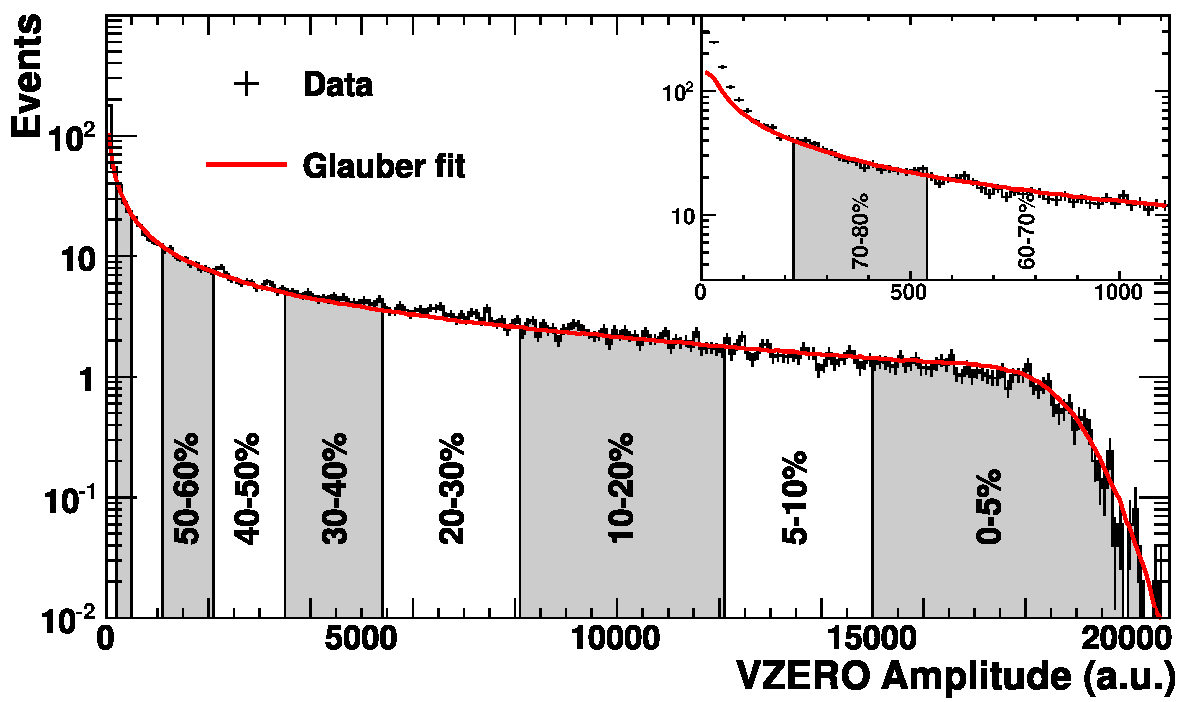
\includegraphics[width=0.5\textwidth]{ksfigures/VZEROCent.pdf}
\caption{Distribution of the sum of amplitudes from the VZERO scintillators in the ALICE experiment (histogram) fitted to Glauber Monte Carlo coupled to NBD multiplicity production model (line). The inset shows peripheral-collision region enlarged. Reproduced from~\cite{Abelev:2013qoq}.}
\label{figks:V0centr}
\end{figure}

Figure~\ref{figks:V0centr} illustrates the result of such a fit to the event distribution of the sum of amplitudes from the VZERO counters (see Sec.~\ref{subsecall:detectors} for detector description) in the ALICE detector. This variable is proportional to the multiplicity in the pseudorapidity region covered by the VZERO detector. The centrality classes and their percentiles are determined by integrating the experimental distribution from its maximal value down to the anchor point. Simulated events are then used to calculate $\langle N_{\rm part} \rangle$ and $\langle N_{\rm coll} \rangle$ for the centrality classes. The ATLAS experiment for the centrality selection is using transverse energy measured in Forward Calorimeters (FCal) and, instead of the model for multiplicity production, the pile-up of calorimeter response from $N_{\rm anc}$ pp collisions is exploited~\cite{ATLAS:2011ag}. The CMS experiment bases its Pb--Pb centrality selection on Hadron Forward (HF) calorimeter, and the distribution of the transverse-energy sum is corrected with the simulation of the trigger response~\cite{Chatrchyan:2011pb}. Another detector commonly used for centrality measurements is the ZDC. Its disadvantage is that, unlike for the multiplicity-type detectors, the ZDC response is not a monotonic function of centrality: it gives small signals both for very central and for very peripheral collisions. ZDC's are therefore normally used in correlation with some other detector, especially for central and very central events.

The centrality determination and its uncertainties affect practically all the results from the analyses of heavy-ion data. A careful systematic study of the centrality selection dependence on different assumptions is always required. This usually includes: variation of the parameters describing the nucleus density, including that for nucleon-exclusion volume, within the uncertainties from~\cite{DeJager:1987qc}; modifying the definition of colliding nucleons (from a black-disc assumption to a Gaussian profile description, or introducing an intra-nuclear rescattering); and changing the functional dependence of $N_{\rm anc}$, if used, to a power function of $N_{\rm part}$ or $N_{\rm coll}$. All these uncertainties must then be properly propagated to the measurements of other quantities.

\subsection{Charged-particle density}
\label{subsecks:partdensity}
Traditionally, the very first measurements of heavy-ion collisions at a new energy regime comprise the charged-particle density, and its centrality dependence. These measurements were performed by all three experiments participating in the LHC heavy-ion programme~\cite{Aamodt:2010pb,Aamodt:2010cz,ATLAS:2011ag,Chatrchyan:2011pb}, and the first results were published already during the first heavy-ion run~\cite{Aamodt:2010pb}. The methods exploited to measure the charged-particle density (${\rm d}N_{\rm ch}/{\rm d}\eta$) in the mid-rapidity region ($|\eta| < 0.5$) were very similar. All experiments used their silicon pixel trackers, detectors closest to the interaction point, to count so called tracklets, pairs of reconstructed hits (pixel clusters) in two layers of the pixel detectors aligned with the primary vertex. Other methods, such as measuring the cluster multiplicity, partial tracking with innermost detectors, and TPC tracking (in the case of ALICE), were also utilized. The collision-energy dependence of ${\rm d}N_{\rm ch}/{\rm d}\eta$ for the most central heavy-ion collisions, normalized per participant pair (i.e. $\langle N_{\rm part} \rangle /2$), is presented in Fig.~\ref{figks:EnrgyMult}, top part. The results from the three experiments are in excellent agreement, and they show an increase by more than factor of two, compared to the highest value observed at RHIC. The energy dependence of the charged-particle density can be satisfactorily parameterized by a power function: $\propto s_{\rm NN}^{0.15}$. Note that the energy dependence for heavy ions is significantly steeper than that for pp interactions ($\propto s^{0.11}$), this is also reflected by the more than a factor two higher value of the normalized charged-particle density $({\rm d}N_{\rm ch}/{\rm d}\eta)/(0.5\langle N_{\rm part} \rangle)$ in heavy-ion collisions compared to pp interactions. It is interesting to note that most of the theoretical and model predictions for the LHC charged-particle density underestimated the experimental observation~\cite{Aamodt:2010pb}, contrary to a clear tendency for an overestimation when the first results from RHIC experiments were published.

\begin{figure}
\centering
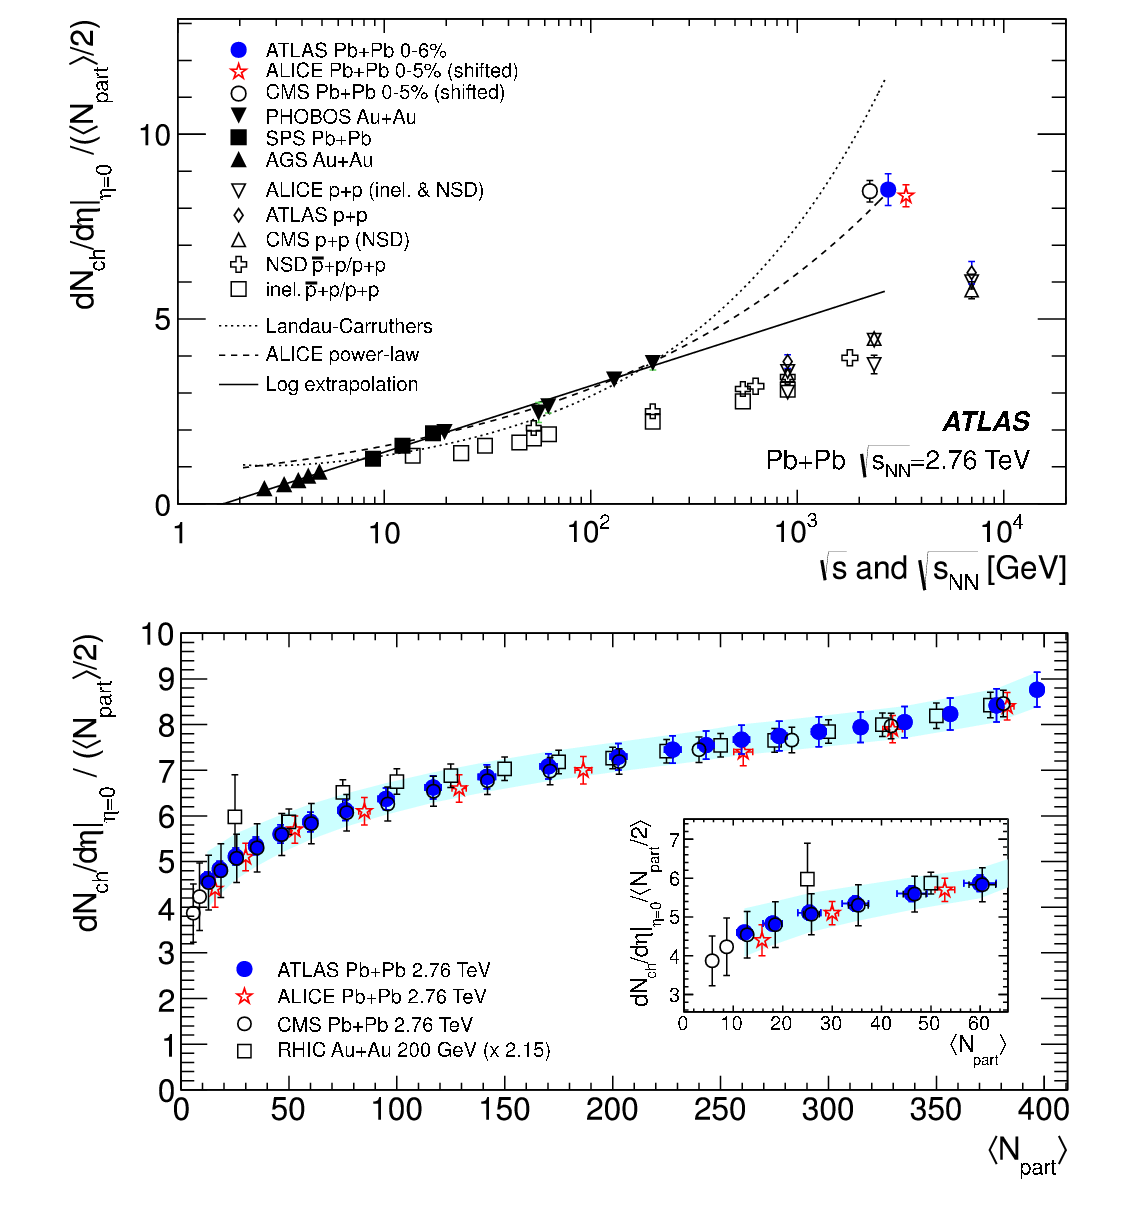
\includegraphics[width=0.5\textwidth]{ksfigures/EnergCentMult.png}
\caption{Top: Energy dependence of the charged-particle density at mid-rapidity ($|\eta| < 0.5$) normalized per participant nucleon pair, from various pp (and $\overline{\rm p}$p) measurements, and most central heavy-ion collisions. The curves represent various extrapolations from lower-energy data to LHC, the one describing heavy-ion experimental points (dashed line) is a power function $({\rm d}N_{\rm ch}/{\rm d}\eta)/(0.5 \langle N_{\rm part} \rangle) \propto s_{\rm NN}^{0.15}$ proposed in~\cite{Aamodt:2010pb}. Bottom: $\langle N_{\rm part} \rangle$ dependence of the charged-particle density normalized per participant nucleon pair from the three LHC experiments, compared to average value from RHIC experiments, multiplied by a factor $2.15$. The shaded band indicates the total systematic uncertainty of the ATLAS measurement (similar to those of the other two LHC experiments),  including $\langle N_{\rm part} \rangle$ uncertainties. The inset shows in detail the peripheral-collision region with $\langle N_{\rm part} \rangle < 60$. Reproduced from~\cite{ATLAS:2011ag}.}
\label{figks:EnrgyMult}
\end{figure}

In the bottom part of Fig.~\ref{figks:EnrgyMult} the centrality dependence of the same quantity $({\rm d}N_{\rm ch}/{\rm d}\eta)/(0.5 \langle N_{\rm part} \rangle)$, expressed as a function of $\langle N_{\rm part} \rangle$, is presented. Again, very good agreement among the three LHC experiments is observed. The data from RHIC (average value over the four experiments~\cite{Adler:2004zn}) are also shown, multiplied by a factor $2.15$ to match the points for the most central collisions. The normalized charged-particle density is rising with centrality, which means that the particle multiplicity at mid-rapidity increases faster than the number of participants, presumably due to the contribution of hard processes to the multiplicity production. However, this increase is very similar to that observed at the top RHIC energy. Apart from a simple interpretation of these data in terms of (a mixture of) soft and hard interactions, model calculations implementing a saturation picture, where the number of soft gluons available for the multiplicity production is progressively reduced by parton recombination, attempt to determine the energy and centrality dependence of the saturation scale~\cite{Armesto:2004ud,Kharzeev:2004if,ALbacete:2010ad}.

The experiments were also looking for the ${\rm d}N_{\rm ch}/{\rm d}\eta$ evolution in the longitudinal direction, i.e. as a function of pseudorapidity. The ATLAS collaboration published the charged-particle densities for different centrality classes in $|\eta| < 2$~\cite{ATLAS:2011ag}, and the CMS detector measured ${\rm d}N_{\rm ch}/{\rm d}\eta$ in the interval $|\eta| < 2.5$~\cite{Chatrchyan:2011pb}. The ALICE experiment extended the pseudorapidity coverage of such measurement to $- 5 < \eta < 5.5$~\cite{Abbas:2013bpa}, exploiting the FMD (see Sec.~\ref{subsecall:detectors}) and so called satellite bunches. The latter are created in the accelerator RF cavities, when a small fraction of particles slips from the main bunch into another wave period, $75$~cm apart (corresponding to RF frequency $400$~MHz). This way, very low-intensity satellite collisions, distanced by every $37.5$~cm from the main bunch crossing, are produced, shifting the pseudorapidity acceptance. Figure~\ref{figks:MultEta} shows the results of the ALICE pseudorapidity distribution measurement, compared to the data previously obtained by CMS and ATLAS. The wide-rapidity data are used together with the RHIC results (from the BRAHMS~\cite{Bearden:2001qq} and PHOBOS~\cite{Alver:2010ck} experiments) to confirm limiting fragmentation --- the shape of the distributions are in the fragmentation region independent of the collision energy. By extrapolation, the total charged-particle multiplicity in Pb--Pb collisions at $\sqrt{s_{\rm NN}} = 2.76$~TeV for different centralities can be estimated, for example, in 5\,\% of the most central events $(17.2 \pm 0.8) \times 10^3$ charged particles are created.

\begin{figure}
\centering
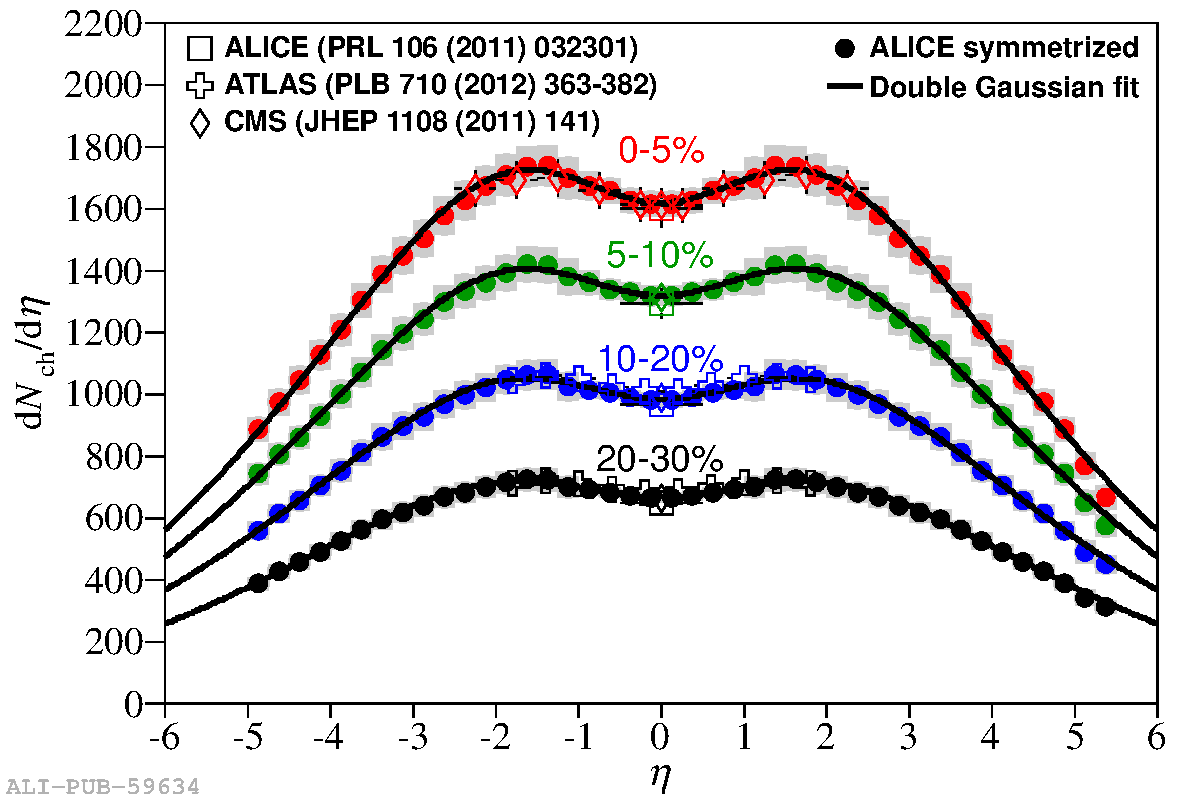
\includegraphics[width=0.5\textwidth]{ksfigures/MultEtaCent.pdf}
\caption{Charged-particle pseudorapidity density distribution for various centrality classes, comparison among the LHC experiments. Reproduced from~\cite{Abbas:2013bpa}.}
\label{figks:MultEta}
\end{figure}


%charged particle density vs energy
%charged particle density vs centrality
%charged particle density vs pseudorapidity
\subsection{Energy density}
\label{subsecks:energydensity}

In order to estimate the energy density achieved in Pb--Pb collisions at the LHC, the measurements of the transverse energy pseudorapidity density, ${\rm d}E_{\rm T}/{\rm d}\eta$ were performed. The CMS experiment measured directly the energy flow in calorimeters for different pseudorapidities and centralities~\cite{Chatrchyan:2012mb}. The collision energy dependence of ${\rm d}E_{\rm T}/{\rm d}\eta$ at mid-rapidity for the most central heavy-ion collisions, normalized to the the number of participant pairs, is shown in Fig.~\ref{figks:ETvsEnerg}. An increase by more than a factor three is observed from the top RHIC energy to the LHC. This collision-energy dependence can be satisfactorily described by a power function $\propto s_{\rm NN}^{0.2}$, which means that the transverse-energy density rises with collision energy faster than the particle density, indicating a significant increase of the average transverse momentum of particles produced in the LHC heavy-ion interactions. The ALICE experiment confirmed the CMS results estimating ${\rm d}E_{\rm T}/{\rm d}\eta$ from ${\rm d}N_{\rm ch}/{\rm d}\eta$ and the measured transverse-momentum spectra for different hadron species~\cite{Collaboration:2011rta}.

\begin{figure}
\centering
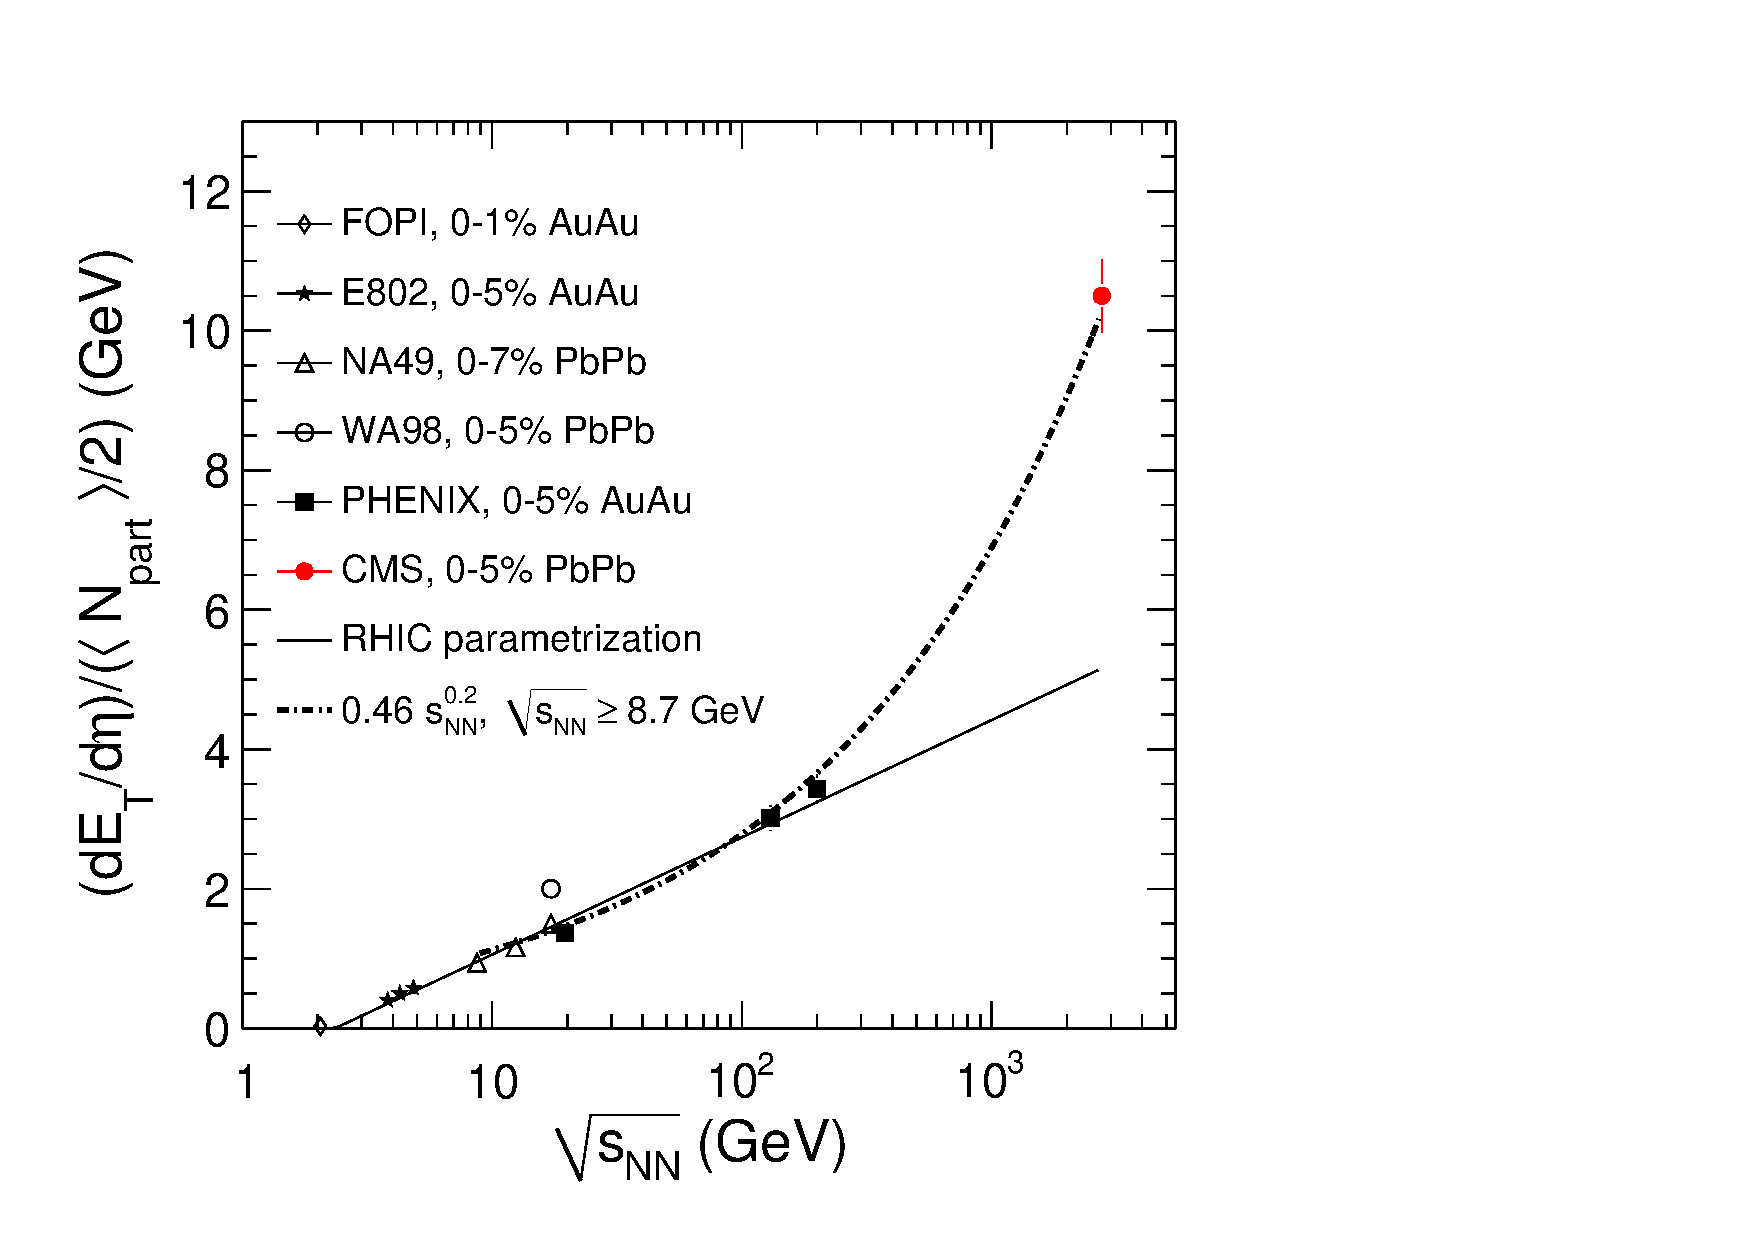
\includegraphics[width=0.5\textwidth]{ksfigures/CMSETvsEnerg.pdf}
\caption{Collision energy dependence of the transverse-energy pseudorapidity density at mid-rapidity, normalized to the number of participant pairs, for central heavy-ion collisions. The curves represent various extrapolations from lower-energy data to LHC, the one describing the LHC measurement (dashed--dotted line) is a power function $({\rm d}E_{\rm T}/{\rm d}\eta)/(0.5 \langle N_{\rm part} \rangle) \propto s_{\rm NN}^{0.2}$ proposed in~\cite{Chatrchyan:2012mb}, from where this figure is reproduced.}
\label{figks:ETvsEnerg}
\end{figure}

Even in forward region, up to $|\eta| = 5$, the transverse-energy density observed at the LHC is larger than that at mid-rapidity at the top RHIC energy. The energy density achieved in heavy-ion interactions ($\epsilon$) is commonly related to the transverse-energy density by the Bjorken formula~\cite{Bjorken:1982qr}, based on geometrical considerations. It can be expressed as $\epsilon \tau_{0} = ({\rm d}E_{\rm T}/{\rm d}y) / S$, where $\tau_{0}$ denotes the time when the initial thermalization was established (supposed to be $\tau_{0} \leq 1$~fm), and $S$ is the transverse overlap area, approximated for central Pb--Pb collisions with $\pi (7\,{\rm fm})^2$. For the top 5\,\% centrality CMS obtained $\epsilon \tau_{0} = 14$~GeV/fm$^2$ (using a model estimation for Jacobian ${\rm d}\eta/{\rm d}y \approx 1.1$). This represents a factor 2.6 increase with respect to the highest RHIC collision energy~\cite{Adcox:2004mh}, and an even larger increase for the energy density $\epsilon$, since the time $\tau_{0}$ is expected to be shorter at the LHC.
%energy density vs energy

\section{Particle spectra and yields}
\label{secks:spectra}
\subsection{Charged-particle spectra}
\label{subsecks:transspectra}
Transverse momentum spectra of charged particles were measured by all three experiments exploiting the first collected data sample. They are presented as the dependence of the (inclusive) invariant cross section on the transverse momentum ($p_{\rm T}$), and finally in the form normalized to pp measurement at the same nucleon--nucleon energy. For the latter representation, the nuclear modification factor is defined as
\be
R_{\rm AA}(p_{\rm T}) = \frac{{\rm d}N_{\rm ch}^{\rm AA}(p_{\rm T})/{\rm d}p_{\rm T}}{\langle N_{\rm coll} \rangle \,{\rm d}N_{\rm ch}^{\rm pp}(p_{\rm T})/{\rm d}p_{\rm T}} ,
\label{eqks:RAA}
\ee
where on the right hand side the superscripts AA and pp refer to the values obtained in heavy-ion and pp measurements, respectively. If a collision of two nuclei behaved as a simple superposition of $N_{\rm coll}$ nucleon--nucleon collisions, the nuclear modification factor would be $R_{\rm AA} = 1$. Such a scaling with the number of binary collision $N_{\rm coll}$ is a natural expectation for hard processes, in case that nucleons act independently and their interactions are not influenced by the rest of the nuclei. This is observed for electro-weak bosons, since they practically do not interact with the surrounding medium, see Sec.~\ref{sect:pas:ew}. A deviation of $R_{\rm AA}$ from unity for hard processes signals a nuclear effect. However, for soft processes, such as particle production at $p_{\rm T}$ below a few GeV, the scaling from pp to AA is governed by $N_{\rm part}$ rather than by $N_{\rm coll}$, leading naturally to an $R_{\rm AA}$ below unity in that $p_{\rm T}$ region, especially for central events.

The $p_{\rm T}$ spectrum for charged particles in LHC heavy-ion collisions was expected to be suppressed at high $p_{\rm T}$ with respect to pp interactions. The fact that $R_{\rm AA}$ is significantly below unity at $p_{\rm T}$ above a few GeV was well established for central collisions at RHIC, and attributed to the jet quenching --- an energy loss of hard partons in their interactions with the surrounding high-density nuclear matter. As the high-$p_{\rm T}$ particles are supposed to be produced in the fragmentation of such hard partons, the shift to lower $p_{\rm T}$  by parton-energy loss decreases the particle production, reflecting the amount of energy loss, and thus the density of nuclear matter created in the collision. However, the value of $R_{\rm AA}$ is also dependent on the steepness of the parton $p_{\rm T}$ spectrum (for fixed parton energy loss, a harder parton spectrum at the LHC should result in less particle suppression), and on the nuclear modification of the structure functions (distribution of partons inside a nucleon). Therefore, for theoretical predictions and interpretations of the $R_{\rm AA}$ behaviour, model calculations taking into account the interplay of many effects are necessary.

The first LHC measurement of charged-particle $R_{\rm AA}$, was published by ALICE~\cite{Aamodt:2010jd}, presenting the $p_{\rm T}$ spectrum up to 20~GeV, for the 5\,\% most central Pb--Pb events. It showed a slightly stronger suppression compared to RHIC: the largest suppression, in the $p_{\rm T}$ range 6--7~GeV, was a factor about 7 at the LHC, while at RHIC a factor of 5 was observed. A new observation was that with increasing $p_{\rm T}$ the suppression gets smaller, i.e. $R_{\rm AA}$ increases. This was soon confirmed by the CMS measurement~\cite{CMS:2012aa}, extending the $p_{\rm T}$ reach up to 100~GeV (see Fig.~\ref{figks:CMSRAA}). The nuclear modification factor $R_{\rm AA}$ exhibits a clear increase up to $p_{\rm T}$ about 40~GeV, and and then seems to saturate with the $R_{\rm AA}$ value about 0.5--0.6 for the most central collisions. Figure~\ref{figks:CMSRAA} also shows the $p_{\rm T}$ dependence of $R_{\rm AA}$ at lower energies, and a variety of model calculations~\cite{Dainese:2004te,Vitev:2002pf,Vitev:2004bh,Salgado:2003gb,Armesto:2005iq,Renk:2011gj}. Different models can be tuned to fairly reproduce the $R_{\rm AA}$ data, however, it remains to be demonstrated that they describe with the same parameters the collision-energy dependence between RHIC and the LHC, and  the ensemble of other observables, especially the azimuthal anisotropy (Sec.~\ref{sec:ps:flow}).

\begin{figure}
\centering
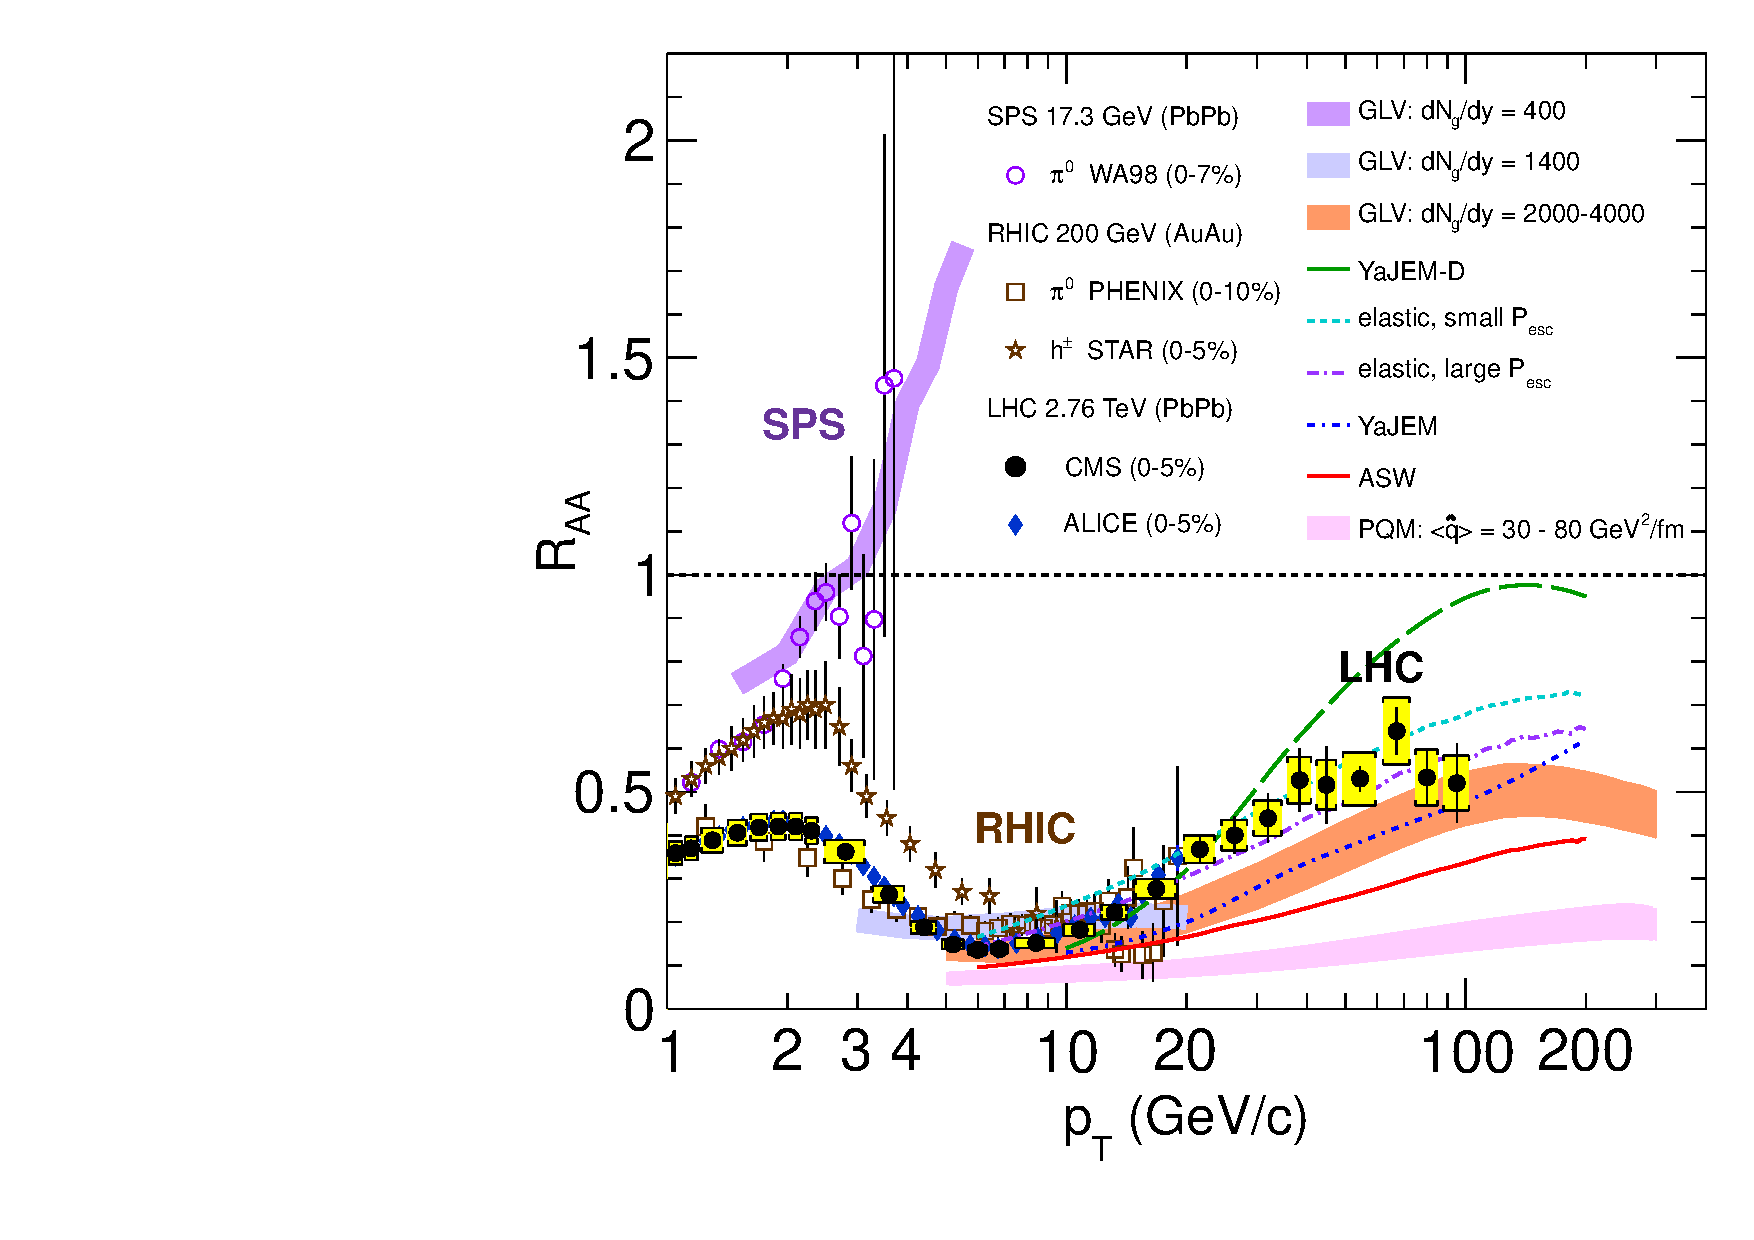
\includegraphics[width=0.5\textwidth]{ksfigures/CMSRAA.pdf}
\caption{Transverse momentum dependence of nuclear modification factor $R_{\rm AA}$ for charged particles produced in central heavy-ion collisions at LHC and lower energies. The curves and bands represent different model calculations. Reproduced from~\cite{CMS:2012aa}.}
\label{figks:CMSRAA}
\end{figure}

The CMS and ALICE experiments also measured the $R_{\rm AA}$ $p_{\rm T}$ dependence for different collision centralities~\cite{CMS:2012aa,Abelev:2012hxa}. The charged-particle production is, as expected, less and less suppressed as one moves from central to peripheral Pb--Pb collisons. The ATLAS collaboration reported similar results, presented as $R_{\rm CP}$ as a function of $p_{\rm T}$, where $R_{\rm CP}$ stands for a quantity analogue  to that defined in Eq.~\ref{eqks:RAA} using the normalized ratio of heavy-ion results at different centralities (the subscript CP indicates the central-to-peripheral ratio), commonly using the most peripheral class available for normalization.
%R_AA from CMS up to 100 GeV
\subsection{Identified-hadron spectra}
\label{subsecks:identspectra}
Study of the particle composition as a function of $p_{\rm T}$ reveals a mass hierarchy, interpreted as resulting from a common radial-velocity field created during the expansion of the dense-matter fireball. Such a collective flow arises in strongly interacting matter in the presence of a pressure gradient. Having the same velocity, heavier particles (e.g. protons) will acquire a larger momentum than lighter mesons. This effect is  visible in Fig.~\ref{figks:IdentPartSpec}, where the $p_{\rm T}$ spectra for pions, kaons, and protons measured by the ALICE experiment~\cite{Abelev:2012wca,Abelev:2013vea} exploiting various particle-identification techniques, are presented for the top 5\,\% central events, and compared to RHIC data~\cite{Adler:2003cb,Abelev:2008ab}. As the slope of the $p_{\rm T}$ spectra is affected by the particle masses ($m$), more instructive is to demonstrate it using the transverse-mass  ($m_{\rm T} = \sqrt{p_{\rm T}^2 + m^2}$) spectra, as done in~\cite{Heinz:2013th}. From the simultaneous blast-wave fit~\cite{Schnedermann:1993ws} to the $p_{\rm T}$ spectra (excluding pions with $p_{\rm T} < 0.5$~GeV and kaons with $p_{\rm T} < 0.35$~GeV where resonance decays largely contribute; more proper way would be to account for resonances and their decays in the fit, this is in preparation), the kinetic freeze-out temperature ($T_{\rm kin}$, temperature when the hadrons cease to interact) and an average radial velocity ($\langle \beta \rangle$) is estimated. The two parameters were extracted for different centralities, and they were found to be strongly correlated, since they both determine the slope of the $p_{\rm T}$ spectra. Both $T_{\rm kin}$ and $\langle \beta \rangle$ are higher compared to RHIC, and they depend on centrality: $T_{\rm kin}$ being lower for more central collisions, while $\langle \beta \rangle$ increases. The values reached for 5\,\% of most central collisions are $T_{\rm kin} \approx 95$~MeV and $\langle \beta \rangle \approx 0.65$, the latter being more than 10\,\% above the RHIC value~\cite{Adams:2005dq}. The blast-wave studies are being improved, sophisticating the model as mentioned above, exploiting data on other particle species, and using various assumptions about which particles have a common $T_{\rm kin}$ and which have a different one (i.e. accounting for differences in cross sections at low energies). Such studies will remain (useful) approximations of full hydrodynamical calculations coupled with a microscopic hadron-transport model.

The $p_{\rm T}$ spectra were compared further to various hydrodynamical-model calculations~\cite{Shen:2011eg,Bozek:2012qs,Werner:2012xh,Karpenko:2012yf}, and a fair description for the bulk production, up to transverse momenta 2--3~GeV, i.e. where such models are applicable, is observed for central collisions. In some cases~\cite{Karpenko:2012yf,Karpenko:2011qn} the agreement is improved by supplementing the hydrodynamical calculations with a hadronic rescattering code (UrQMD~\cite{Bass:1998ca}, in this occasion). The Krakow model~\cite{Bozek:2011ua,Bozek:2011gq} uses bulk viscosity corrections at freeze-out to describe deviation from equilibrium, which seems successful in reproducing the data. But going to more peripheral collisions the hydrodynamical description becomes worse at higher $p_{\rm T}$ and shows the limits of the hydrodynamical models. This could indicate the onset of a non-thermal (hard) component, which in more peripheral collisions is not dominated by the flow-boosted thermal component~\cite{Bozek:2012qs}.

\begin{figure}
\centering
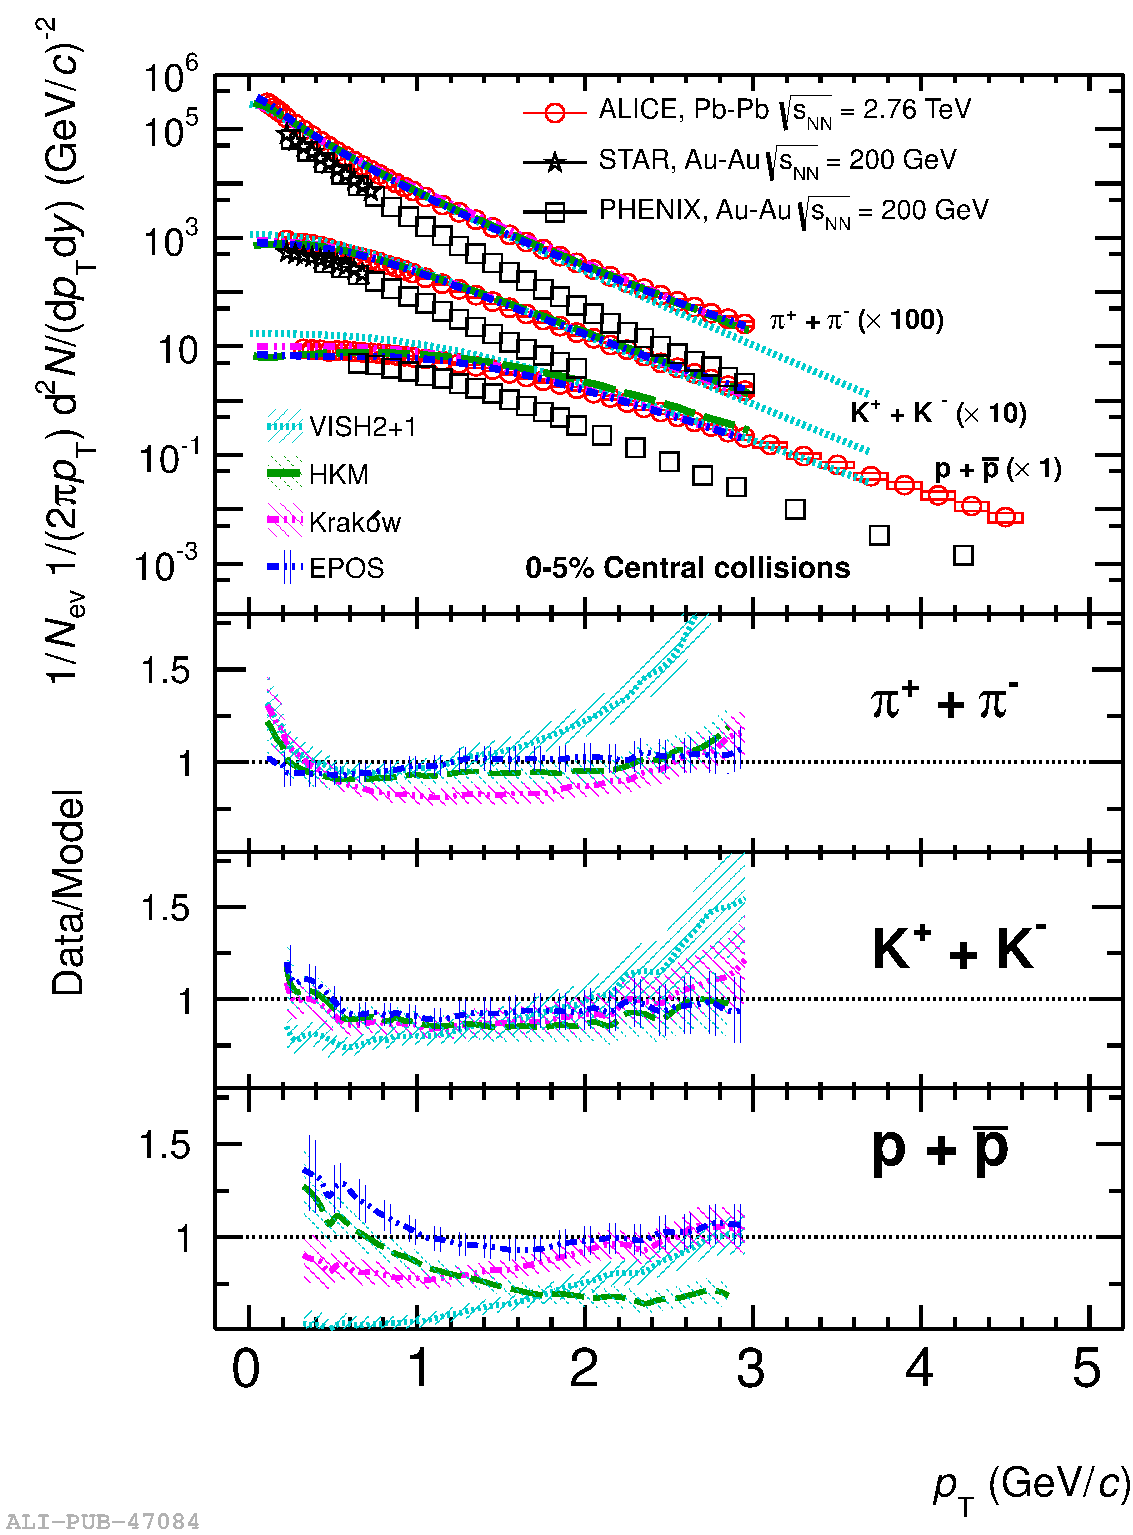
\includegraphics[width=0.5\textwidth]{ksfigures/IdentPartSpec.pdf}
\caption{Transverse momentum spectra for pions, kaons, and protons (sum of particles and antiparticles) produced in 5\,\% of most central Pb--Pb collisions at LHC, compared to the RHIC measurements and different model calculations. Adapted from~\cite{Abelev:2012wca}.}
\label{figks:IdentPartSpec}
\end{figure}

\begin{figure}
\centering
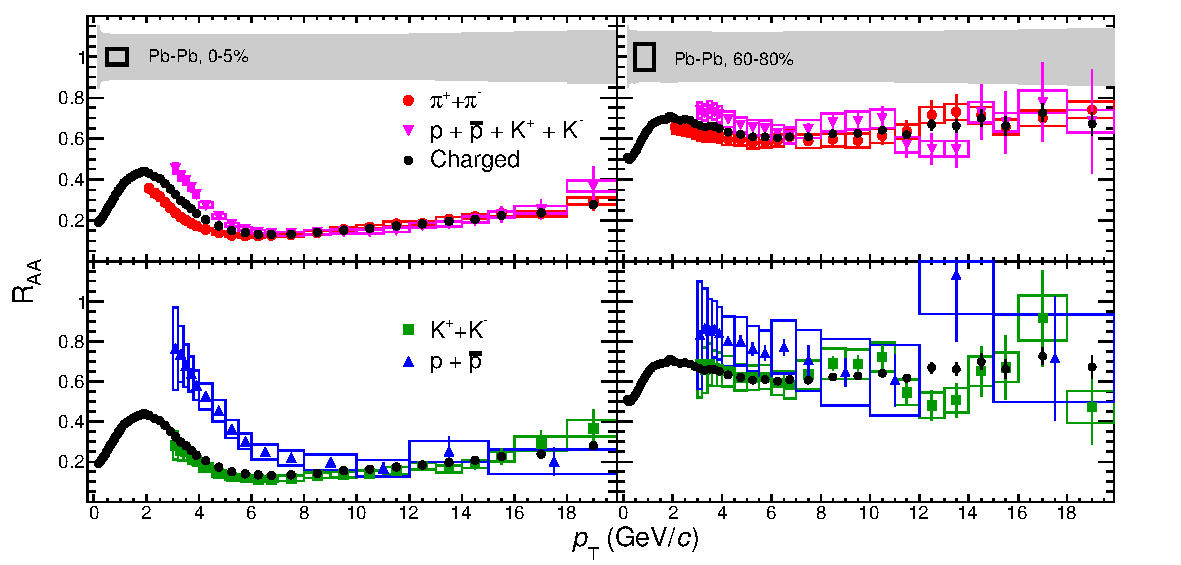
\includegraphics[width=0.75\textwidth]{ksfigures/IdentHighPtRAA.pdf}
\caption{Nuclear modification factor $R_{\rm AA}$ for pions, kaons, and protons (sum of particles and antiparticles), and averaged for charged particles, as a function of $p_{\rm T}$ for central (left, 0--5\,\%) and peripheral (right, 60--80\,\%) Pb--Pb collisions. Reproduced from~\cite{Abelev:2014laa}.}
\label{figks:IdentPartRAA}
\end{figure}

The $p_{\rm T}$ spectra of identified charged hadrons are determined up to $p_{\rm T} = 20$~GeV~\cite{Abelev:2014laa}, exploiting the measurement of ionization energy losses in the ALICE TPC in the relativistic rise region. Figure~\ref{figks:IdentPartRAA} presents these results normalized to the pp baseline, as $R_{\rm AA}$ for pions, kaons, and protons, compared to the (averaged) charged-particle data. It is clearly seen that for $p_{\rm T}$ above 7--8~GeV the behaviour for all particle species coincides. For lower $p_{\rm T}$ a mass hierarchy appears: the heavier the particle, the lower its suppression. These observations suggest the presence of three regions in transverse momentum:
\begin{itemize}
    \item{bulk region, low $p_{\rm T}$ up to 2--3~GeV, where the production comes from the hadronization of high-density strongly-interacting matter created in a heavy-ion collision, reflecting collective radial flow, fairly described (at least for central collisions) by hydrodynamical models;}
    \item{intermediate region, in $p_{\rm T}$ up to 7--8~GeV, where still a mass splitting among various particle species persists that can be attributed a reminiscence of radial flow (the difference has to disappear for $p_{\rm T}$ values significantly larger than particle masses), however, additional ideas were put forward to push further in $p_{\rm T}$ this mass distinction, such as constituent-quark recombination~\cite{Hwa:2006zq} which would favour baryons to acquire larger $p_{\rm T}$ than mesons;}
    \item{fragmentation region, above 7--8~GeV in $p_{\rm T}$, where the different hadron species exhibit a common suppression pattern, and consequently their relative abundances are the same as in pp collisions, naturally explained as being fragmentation products of a high-$p_{\rm T}$ parton coming from a hard scattering at early stage (which itself is quenched by the surrounding high-density matter).}
\end{itemize}

\begin{figure}
\centering
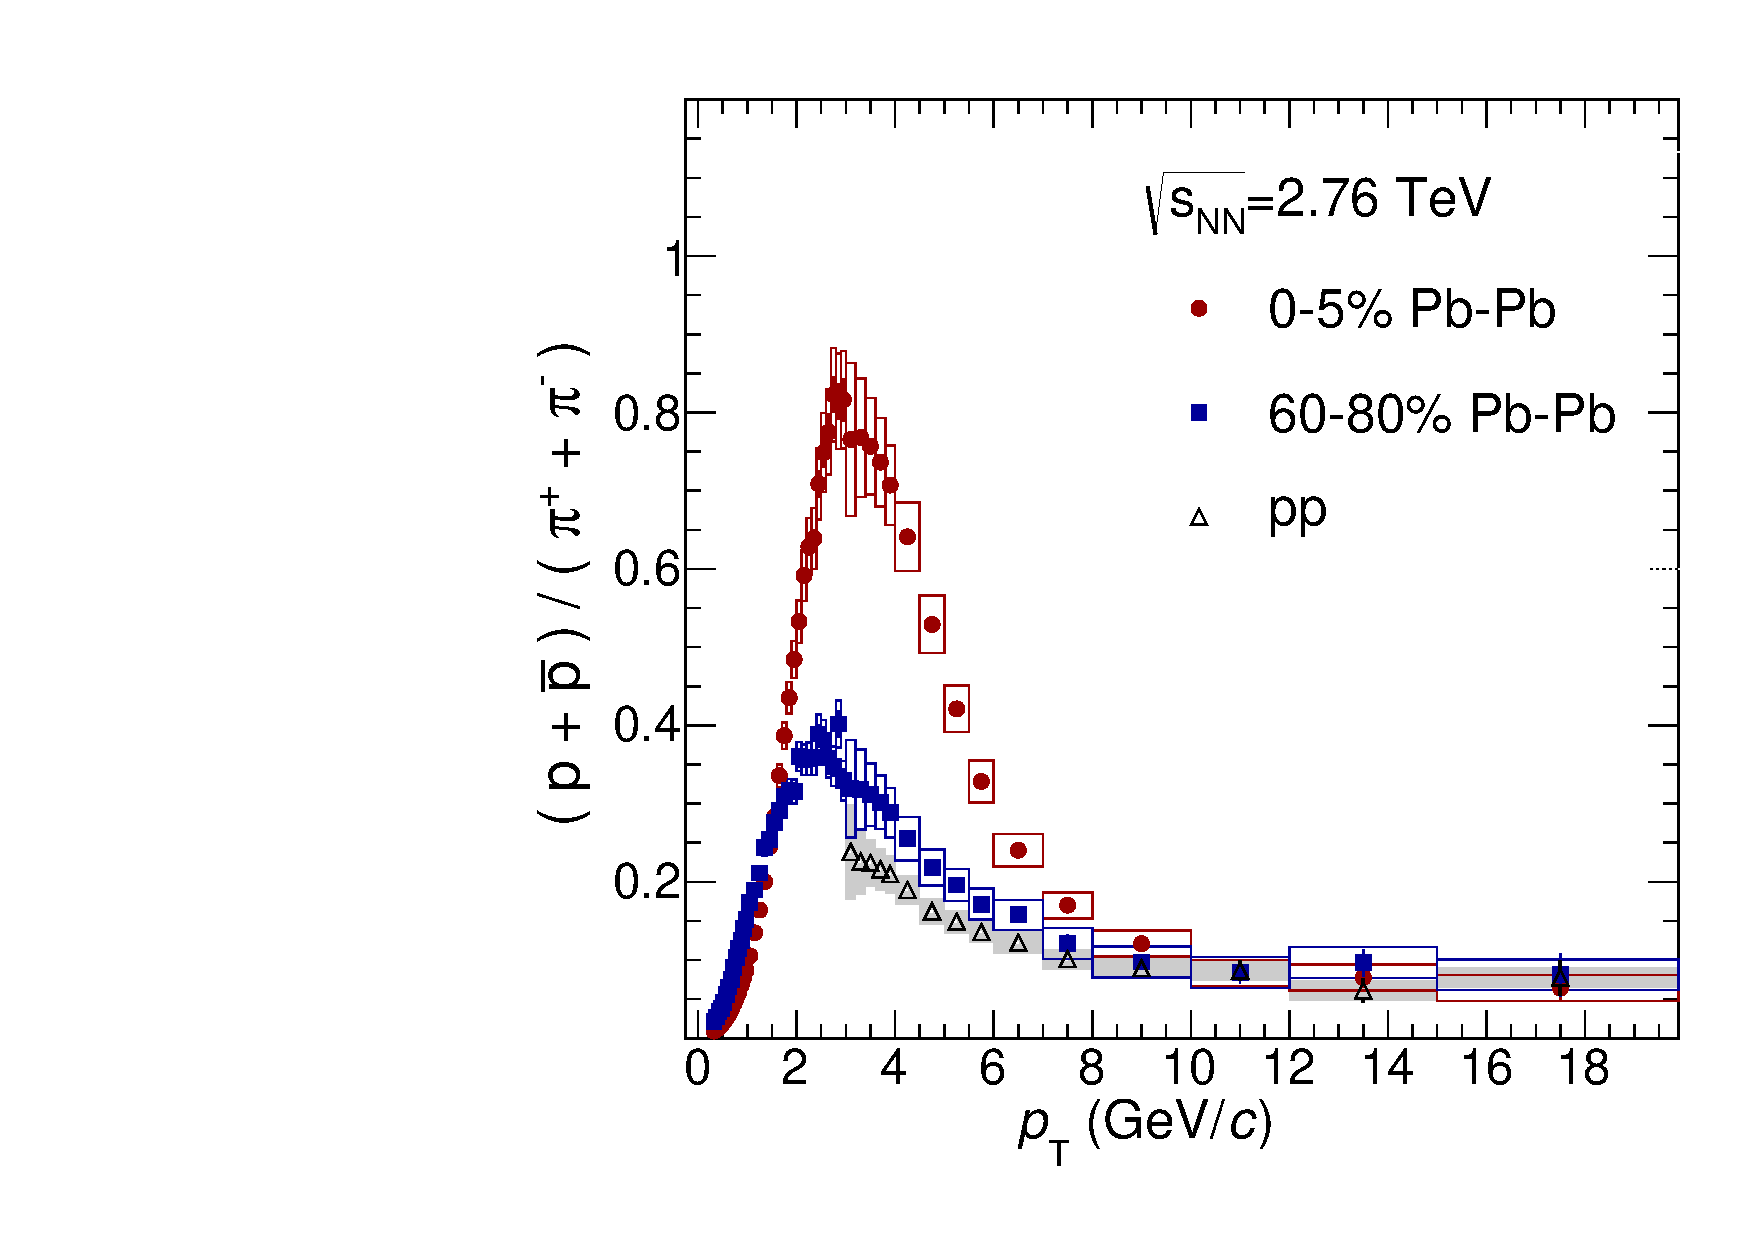
\includegraphics[width=0.5\textwidth]{ksfigures/ProtonToPion.pdf}
\caption{Ratio of proton-to-pion yields as a function of $p_{\rm T}$ measured in central (0--5\,\%) and in peripheral (60--80\,\%) Pb--Pb collisons, and in pp collisions. Reproduced from~\cite{Abelev:2014laa}.}
\label{figks:ProtonToPion}
\end{figure}

To look in detail into the intermediate region, it is instructive to plot the proton-to-pion ratio as a function of $p_{\rm T}$, Fig.~\ref{figks:ProtonToPion}. The striking effect is that for central collisions at $p_{\rm T}$ around 2.5--3~GeV this ratio is more than a factor three higher than the value for pp collisions. This so-called baryon anomaly was observed already at RHIC~\cite{Abelev:2006jr,Adare:2013esx}, and certainly the low-$p_{\rm T}$ rise is explained by the hydrodynamical radial flow. In the intermediate region, where the hydrodynamics ceases to work (at $p_{\rm T}$ around 2~GeV), still the hydrodynamic radial flow continues to affect the baryon-to-meson ratio towards higher $p_{\rm T}$, and the behaviour is qualitatively described by models involving constituent-quark recombination~\cite{Fries:2003kq} or baryon string-junction transfer along the axis of a fragmenting jet~\cite{Aurenche:2011rd}. These models, however, tend to predict an anomalous baryon-to-meson ratio even for significantly higher $p_{\rm T}$ than actually observed. On the other hand, a smooth connection between the hydro-described bulk region and the normal-ratio fragmentation region, using a realistic radial-flow profile, will probably move the border between the intermediate and fragmentation regions to lower than observed values. Therefore, a comprehensive description of the particle production in the intermediate region is still an open, and experiment driven issue. Recently, a good description has been obtained
by EPOS model~\cite{Werner:2012xh}, where the interaction between bulk matter (which thermalizes and flows) and jets is considered.

%Pion, Kaon, proton R_AA up to 20 GeV
%pi/p baryon anomaly
\subsection{Strange-particle production}
\label{subsecks:strangespectra}
Historically, the enhancement of strangeness production was among the first signatures proposed to signal a qualitatively different state of matter, expected to be created in ultra-relativistic heavy-ion collisions~\cite{Rafelski:1982pu,Koch:1986ud}. The strangeness increase in high-temperature QCD matter is motivated by two reasons: the relevant quark masses drop from their constituent to their bare values, and then the strange-quark mass becomes comparable to the temperature, consequently the production rates for different light quarks tend to equalize. Strangeness enhancement was already observed at lower energies, e.g. at the SPS~\cite{Margetis:2000sv,Andersen:1999ym,Antinori:2010jm,Alt:2008qm}, as well as at RHIC~\cite{Abelev:2007xp}. The systematic study of strangeness production at the LHC is under way in ALICE~\cite{ABELEV:2013zaa,Abelev:2013xaa}. In addition to charged kaons, the measurements include topologically identified particles (K$_{\rm s}^0$, $\Lambda$, $\Xi^-$, and $\Omega^-$), and resonances containing strangeness.

\begin{figure}
\centering
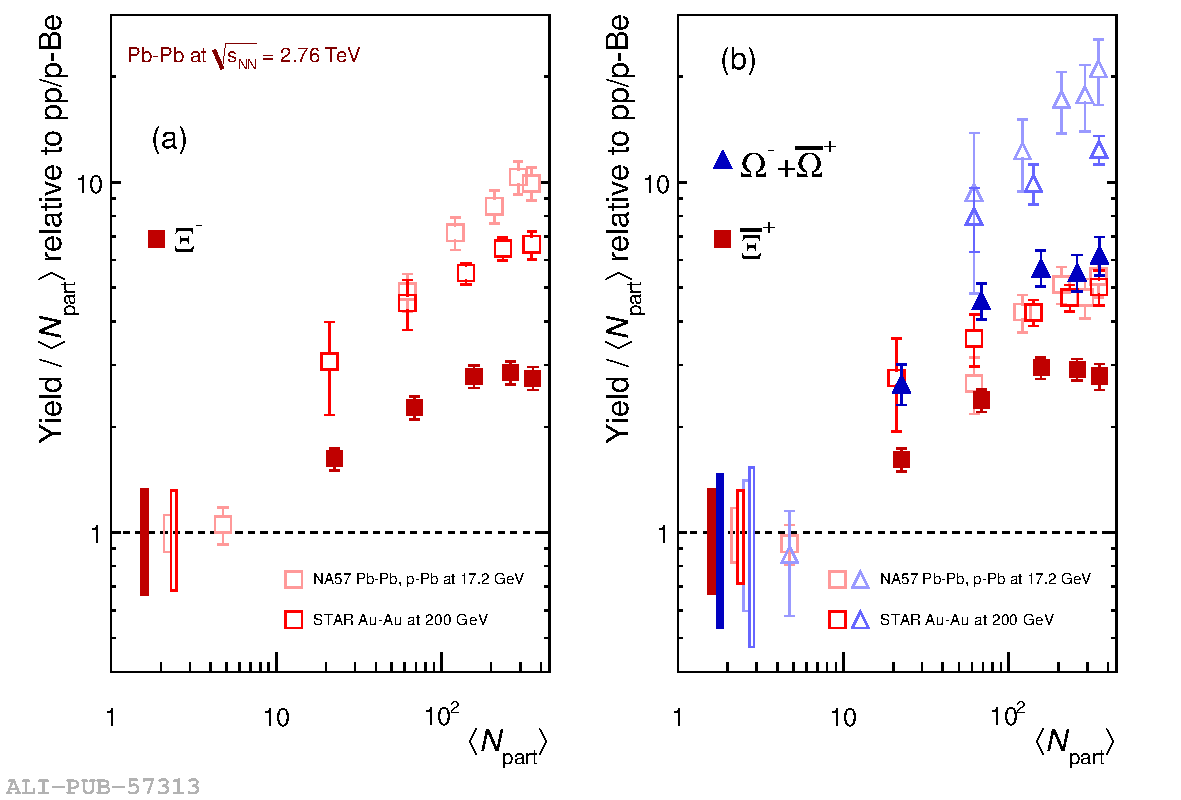
\includegraphics[width=0.75\textwidth]{ksfigures/StrangenessEnhancemet.pdf}
\caption{Strangeness enhancement for $\Xi$ and $\Omega$ at the LHC as the function of the mean number of participants, compared to the results obtained at CERN SPS and RHIC. Reproduced from~\cite{ABELEV:2013zaa}.}
\label{figks:StrangeEnhancement}
\end{figure}


The enhancement of strangeness production is confirmed at the LHC, see Fig.~\ref{figks:StrangeEnhancement}, albeit the enhancement factor, expressed as the ratio of the yield per participant in AA collisions to that in pp (or pA) collisions, decreases slowly with the collision energy. This reflects the fact that the production of strange particles per pion in heavy-ion collisions practically saturates as $\sqrt{s_{\rm NN}}$ reaches few tens of GeV (i.e. the top SPS energy), while in pp it still increases from RHIC to the LHC, and only at the highest energy ($\sqrt{s} = 7$~TeV) seems to cease its growth. However, these asymptotic yields per pion are significantly higher in heavy-ion collisions than in pp interactions, signaling the change of the mechanism of strangeness production. As predicted, to achieve such an increase, roughly a factor of two more strange quarks is necessary, compared the extrapolation from pp collisions. The strange-particle yields are well described by statistical hadronization models (Sec.~\ref{subsecks:yields}) without any strangeness suppression factor, needed in the case of pp and pA collisions.

The strange-particle $R_{\rm AA}$ is also influenced by strangeness enhancement, especially in the bulk and intermediate $p_{\rm T}$ regions~\cite{Knospe:2013tda}. As already mentioned, kaons, including K$_{\rm s}^0$, are above the pion curve. The strange baryons have larger $R_{\rm AA}$ than protons, and $R_{\rm AA}$ increases with the strangeness content, exceeding unity for $\Omega^-$. With increasing $p_{\rm T}$, the strangeness $R_{\rm AA}$ goes progressively closer to the common fragmentation behaviour for all other particle species, still being for $\Omega^-$ at $p_{\rm T} \approx 7$~GeV above the others. These measurements are at this point limited by the available statistics.

\begin{figure}
\centering
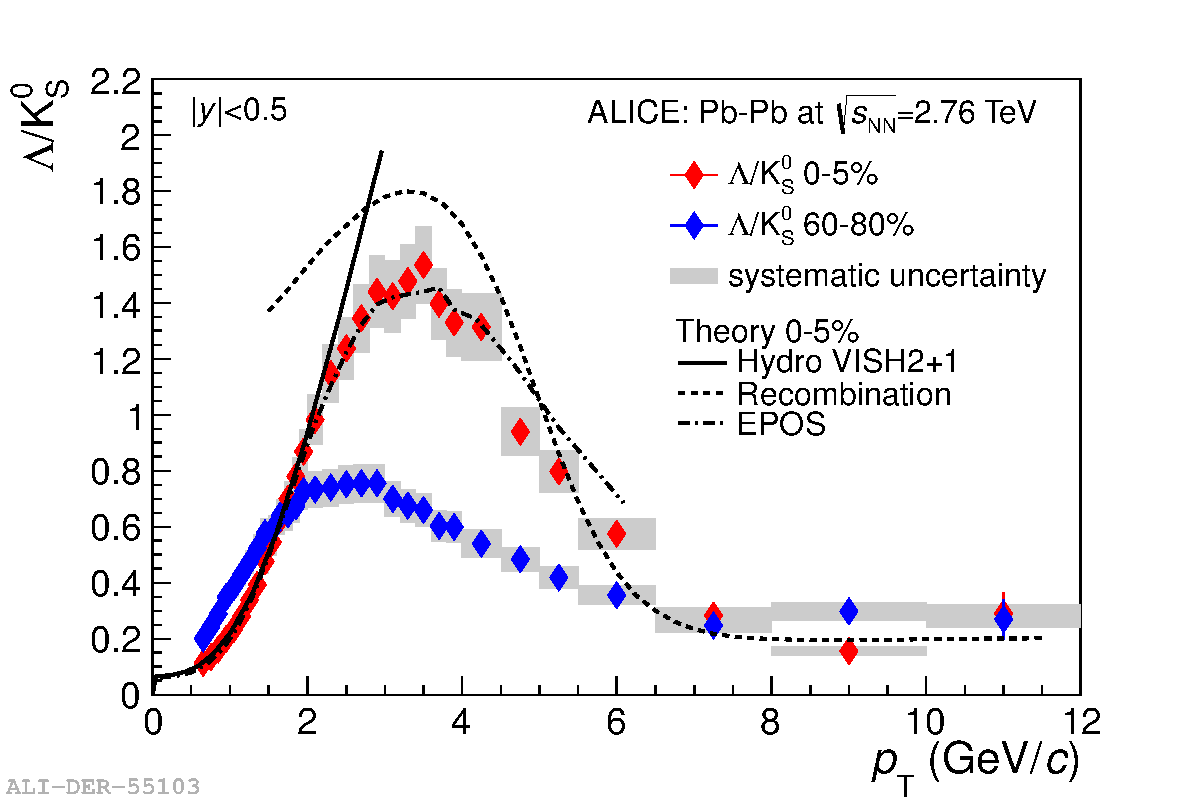
\includegraphics[width=0.5\textwidth]{ksfigures/LambdaToK0T.pdf}
\caption{Ratio of $\Lambda$-to-K$_{\rm s}^0$ yields as a function of $p_{\rm T}$ measured in central (0--5\,\%) and in peripheral (60--80\,\%) Pb--Pb collisons compared to model calculations. Reproduced from~\cite{Abelev:2013xaa}.}
\label{figks:LambdaToK}
\end{figure}


Baryon-to-meson ratio in the strangeness sector is very similar to that of proton-to-pion. The $\Lambda$-to-K$_{\rm s}^0$ ratio as a function of $p_{\rm T}$ is shown in Fig.~\ref{figks:LambdaToK} together with hydrodynamical- and recombination-model calculations~\cite{Song:2007ux,Song:2008si,Song:2011qa}. The EPOS model~\cite{Werner:2012sv}, which includes the hydrodynamical expansion and, at higher $p_{\rm T}$, the (mini-)jet fragmentation with an interaction between jets, describes the experimental measurement fairly well.
%K0, Lambda, Xi, Omega R_AA
%Lambda, Xi, Omega enhancements
%K0/Lambda
\subsection{Resonance and light-nuclei production}
\label{subsecks:resonace}
The resonances are interesting to study in heavy-ion collisions, because of their short lifetime they may decay inside the medium, before the kinetic freeze-out. If a decay product scatter changing its momentum, the parent resonance  cannot be observed by invariant-mass reconstruction, and that leads to an apparent depletion of the resonance yield, which is dependent on the resonance lifetime. On the other hand, resonances can be also recreated during the elastic scattering phase having a large cross-section for $s$-channel production at very low energies. Therefore, the comparison of the different-lifetime-resonance yields with hadronic-transport models gives valuable information about the time evolution during the late stage of heavy-ion collisions.

At the LHC, the ALICE collaboration reported the measurements of K$^*(892)^0$ and $\phi$ mesons~\cite{Abelev:2014uua}. The yield of K$^{*0}$ relative to other particles (e.g. K$^-$) decreases significantly for more central collisions, while the $\phi$ yield normalized in the same way is compatible with being independent of centrality. This is qualitatively understood by an order of magnitude different lifetimes for the two resonances (4.2~fm and 46~fm for K$^{*0}$ and $\phi$, respectively). A substantially lower production of K$^{*0}$ in central collisions also means that the regeneration is not effective enough to compensate the decay rate. Similar observations were made at RHIC~\cite{Aggarwal:2010mt}. The $\phi$ meson, being relatively long-lived to be treated as stable on the time scale of the heavy-ion collision, is of special interest. Its mass is close to that of the lightest baryons, therefore, the $\phi$ $p_{\rm T}$ spectrum can differentiate mass-dependent effects and constituent-quark-number effects. When compared to various hydrodynamical-model calculations~\cite{Shen:2011eg,Qiu:2011hf,Bozek:2012qs,Song:2012tv,Song:2013qma,Karpenko:2011qn,Karpenko:2012yf}, in general, the measured $\phi$ yields are overpredicted. In particular, the VISHNU model (VISH2+1 coupled to UrQMD)~\cite{Song:2012tv,Song:2013qma} is at lower $p_{\rm T}$ (below 1.5~GeV) by a factor of two above the data (probably due to an overestimated regeneration of $\phi$ in the hadronic phase), and fails to describe the shape of the $p_{\rm T}$ distribution. The Krakow model~\cite{Bozek:2012qs} and HKM (hydrokinetic model --- ideal hydrodynamic coupled to UrQMD)~\cite{Karpenko:2011qn,Karpenko:2012yf} are much closer to the data. The experimental results, presented in Fig.~\ref{figks:PhiTop}, indicate compatibility between proton and  $\phi$ $p_{\rm T}$ spectra up to 5~GeV in 10\,\% of most central Pb--Pb collisions, favouring thus the radial-flow explanation of the baryon anomaly to the constituent-quark-recombination one. At RHIC, from $\phi$ elliptic-flow and $p_{\rm T}$-spectrum measurements other conclusion was reached~\cite{Abelev:2007rw}. In peripheral collisions, the proton-to-$\phi$  ratio is not constant (see Fig.~\ref{figks:PhiTop}), possibly implying that the quark content may influence a particle-production mechanism.

\begin{figure}
\centering
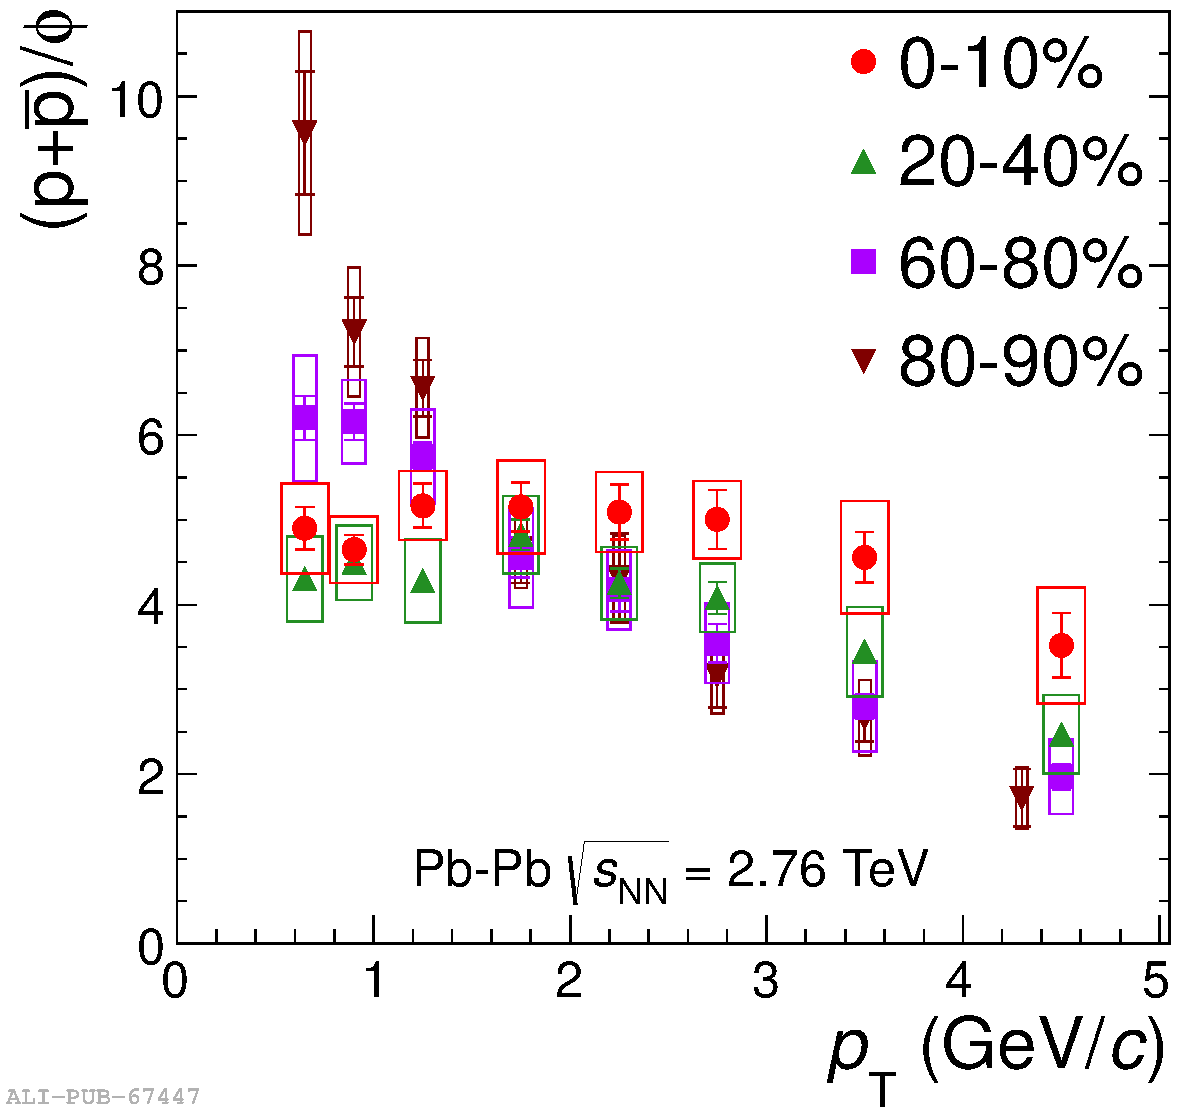
\includegraphics[width=0.5\textwidth]{ksfigures/ProtonToPhi.pdf}
\caption{Ratio of proton-to-$\phi$ yields as a function of $p_{\rm T}$ measured for four centrality intervals in Pb--Pb collisons. Reproduced from~\cite{Abelev:2014uua}.}
\label{figks:PhiTop}
\end{figure}

The high density of particles produced in heavy-ion collisions implies substantial rates for light-nucleus and hypernucleus production. The interest of such measurement is to study the production mechanism of such state, their coalescence coefficients, and their thermodynamical equilibrium with other particles. The light nuclei, such as d, t, $^3$He, and $^4$He, and corresponding antinuclei, were observed in heavy-ion collisions at RHIC and the LHC, and quantitative results for d and $^3$He were reported by ALICE. These measurements use the particle identification based on the specific ionization losses in TPC and the TOF measurement. The production of hypernuclei (nuclei containing one or more strange baryons) is of additional interest since the (unknown) properties of hypernuclei, their masses and decays, can be measured. The ALICE collaboration reconstructed the $^3_{\Lambda}{\rm H} \rightarrow ^3{\rm He} + \pi^-$ decays, as well as the charge-conjugated ones, opening the study in this field at the LHC, following the first antihypertriton measurement at RHIC~\cite{Abelev:2010rv}. Searches for more exotic states, such as the H-dibaryon ($\Lambda\overline{\Lambda}$ bound state or six-quark state), the $\overline{\Lambda}\overline{\rm n}$ bound state, and the $\Phi(1860)$ pentaquark have not given any positive signal.
%phi, deuteron, He3 He4
\subsection{Particle yields}
\label{subsecks:yields}
%particle yields vs thermal models
The particle yields at mid-rapidity are obtained by integration of the transverse-momentum spectra fitted to the blast-wave functional dependence (or other suitable function), in order to extrapolate below the lowest measured $p_{\rm T}$. Traditionally, the particle yields in heavy-ion collisions are studied within statistical hadronization models~\cite{Andronic:2008gu,Andronic:2011yq,Cleymans:1998fq,Becattini:2009fv}. These models are based on the grand-canonical ensemble, describing the system with the temperature ($T_{\rm ch}$), the baryon chemical potential ($\mu_{\rm b}$), and the volume in thermal and chemical equilibrium with the rest. Knowing these parameters it is straightforward to calculate the average number of various particles in the system. All the resonance and other unstable states, summed-up in the grand potential (usually with an upper mass cut-off about $2$~GeV, as above the resonance spectrum is not well known), are decayed into observed particles and compared to the measurements. The temperature $T_{\rm ch}$ is interpreted as the chemical freeze-out temperature, below which the energy of hadronic re-scattering is lower than the threshold for inelastic interactions, and thus the particle composition remains unchanged. The assumption of a chemical freeze-out temperature common to all particle species surmises that the particle composition in a heavy-ion collisions is fixed in a very narrow entropy-density window during the expansion of the high-density and high-temperature fireball.

The statistical models were used to describe the heavy-ion collision data from very low energies up to RHIC with a good agreement for most of the particle species. The temperature $T_{\rm ch}$ practically does not change with the collision energy, therefore, a reasonable estimate for LHC is the value observed at RHIC, $T_{\rm ch} = 164$~MeV; the chemical potential has to be very low as the ratio of particles to antiparticles is for all species compatible with unity; $\mu_{\rm b} = 1$~MeV is usually assumed. The predictions using these parameter values are compared in Fig.~\ref{figks:YieldProtonKaon} with the measurements of yield ratios: p$/\pi$ and K$/\pi$, for different centralities (expressed by particle density). The conclusion is that the measured proton yield for central Pb--Pb collisions at the LHC is by a factor of about 1.5 lower than predicted. In order to describe the proton measurement, significantly lower $T_{\rm ch}$ is needed (about 152~MeV), but then the yields of multi-strange baryons are underestimated. Trying to fit the temperature to the available data gives an estimate of $T_{\rm ch} \approx 156$~MeV, however, the fit description is not as good as it was at lower energies. Moreover, it is hard to expect that the chemical freeze-out temperature would decrease at higher energy.

\begin{figure}
\centering
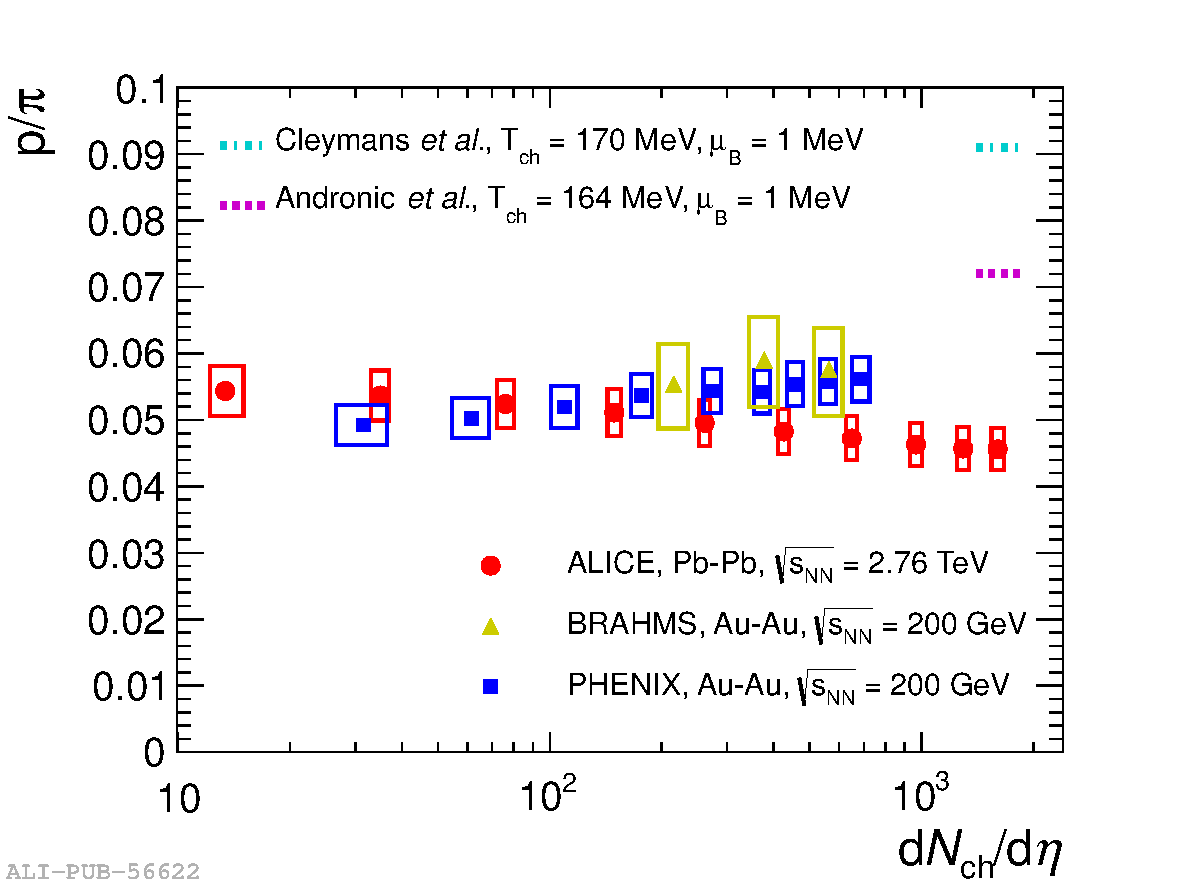
\includegraphics[width=0.4\textwidth]{ksfigures/YieldProtonToPion.pdf}
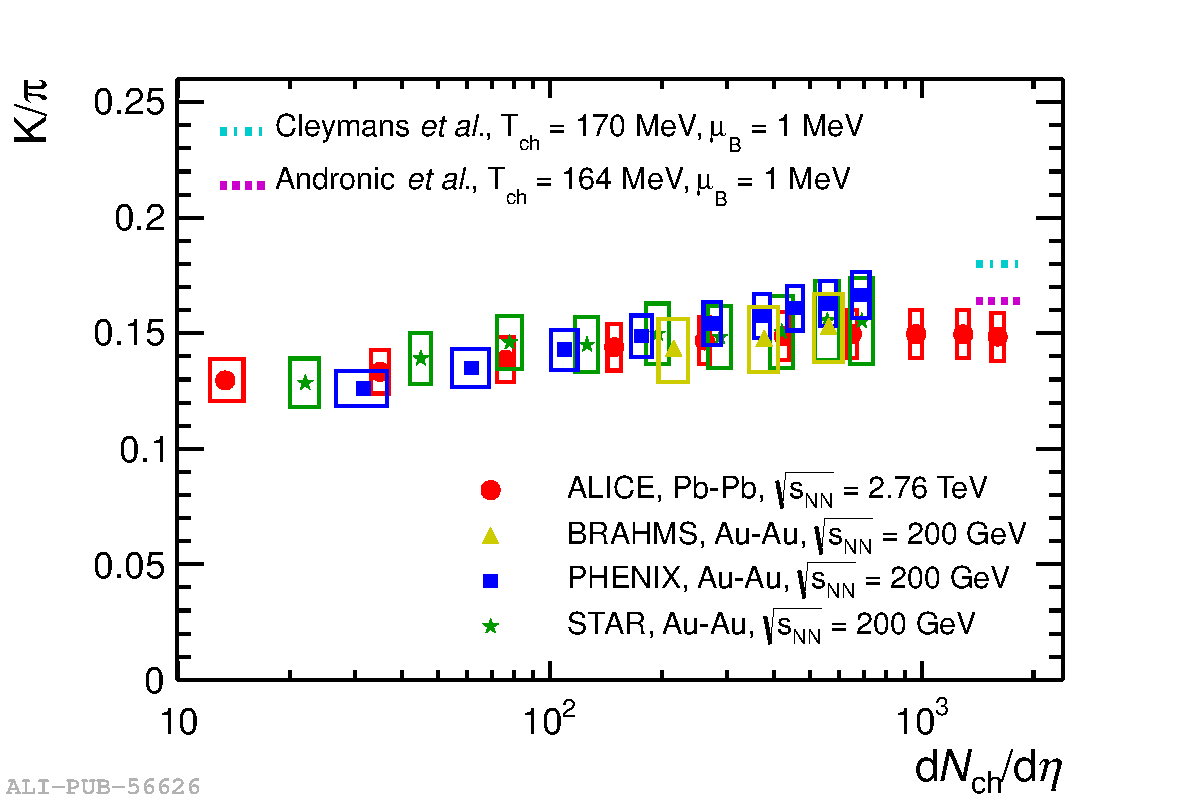
\includegraphics[width=0.4\textwidth]{ksfigures/YieldKaonToPion.pdf}
\caption{Ratios of proton-to-pion (left) and kaon-to-pion (right) yields at mid-rapidity as a function of charged-particle density in Pb--Pb collisons compared to the RHIC measurements~\cite{Abelev:2008ab,Bearden:2001qq,Adler:2003cb}. Reproduced from~\cite{Abelev:2013vea}.}
\label{figks:YieldProtonKaon}
\end{figure}


It seems that such problems were there partly already at RHIC. The discrepancy being smaller, and uncertainties in proton-yield corrections, lead to the fact that it was considered not significant. There are a few attempts to explain the lower proton yield at the LHC:
\begin{itemize}
\item{The baryons can annihilate in re-scattering with antibaryons, even after chemical freeze-out. This will affect protons more then strange baryons, because protons have larger density, and the annihilations with a strange partner are penalized due to presence of kaon(s) in final state, which shrink the phase space and thus lower the cross section of such cross-flavour annihilation. The effect was confirmed with UrQMD calculations~\cite{Karpenko:2012yf,Steinheimer:2012rd,Becattini:2012xb}, and the longer lifetime of the hadron gas makes it larger at the LHC than at RHIC. It was also shown that multi-meson interactions, recreating the baryon--antibaryon pairs, are not, at decreasing temperature, effective enough to compensate the loss~\cite{Pan:2012ne}.}
\item{The statistical hadronization model assumes strictly the same $T_{\rm ch}$ for all particles, which may not necessarily be true. Motivated by recent lattice QCD calculations, flavour- and mass-dependent prehadronic states in QGP may alter the effective phase-transition temperature resulting in an non-uniform freeze out~\cite{Ratti:2011au}. This will consequently modify the yields predicted by the model.}
\item{The high-mass resonances, not accounted for in the model, would presumably increase mostly the pion yield. Because of the number of these resonances can raise exponentially with the mass~\cite{Hagedorn:1965st,RHagedorn:1968}, even their production being exponentially damped, the effect may be non-negligible. This would lower the p$/\pi$ model prediction~\cite{Andronic:2008gu}, however, in a similar way at the LHC and at RHIC.}
\item{The statistical hadronization model can be modified, incorporating non-equilibrium effects. In fact the model was used also to describe particle yields in pp, and even in e$^+$e$^-$, interactions, however, an additional parameter suppressing strangeness production had to be used. Introducing two parameters regulating the population of phase space, separately for light-quarks and strange quark, allows for good description of the experimental measurements.~\cite{Rafelski:2010cw,Petran:2013lja}}
\end{itemize}
The lower-than-expected proton yield observed at the LHC was one of the first surprises from the heavy-ion programme, and its origin has yet to be established.

%... not sign for a large experimental discrepancy between RHIC and the LHC...

\section{Non-flow correlations}
\label{secks:nonflow}
In this section various types of particle correlations, which are not caused by a collective behaviour developed in strongly interacting matter, are discussed. These are typically two-, or a few-, particle correlations arising due to a quantum interference, an interaction between the particles, a common source of production, such as a resonance decay, and a string or (mini-)jet fragmentation. The study of this type of correlations gives information about the space--time evolution of the system, and may shed light on particular production mechanisms.
\subsection{Femtoscopic correlations}
\label{subsecks:femto}
The term femtoscopy is often employed to indicate methods to measure spatial and time scales at a ${\cal O}(1)$~fm level. Basically, two effects are exploited: interference between identical particles and final state particle interactions. The identical-particle interference is consequence of the symmetrization of the wave function. It is connected to the Hanbury-Brown and Twiss (HBT) method proposed to measure stellar sizes~\cite{HanburyBrown:1954wr}, therefore it is sometimes called also in the heavy-ion field HBT method. The production of identical bosons (e.g. pions) with close momenta will be enhanced by such an effect, and that of identical fermions (e.g. protons) will be suppressed. The correlation length in the momentum space is inversely proportional to the spatial size of the source region, assuming that the particles are emitted incoherently. However, the measured correlation is affected by other effects, such as Coulomb interactions, resonance decays, and final state particle interactions, which have to be duly taken into account in the analyses. The latter effect, being often of a short-range nature and present also for non-identical particles, can itself be exploited for femtoscopic studies.

The first results were obtained for like-sign pion--pion correlations with early Pb--Pb data at the LHC~\cite{Aamodt:2011mr}. The analysis was performed in three dimensions, decomposing the relative momentum between the two pions in the longitudinally co-moving system (centre-of-mass system boosted along the beam direction such that the two-pion longitudinal momentum is zero) into its `out' (direction of the momentum of the pion pair), `side' (direction perpendicular to the pair momentum and the beam axis), and `long' (along the beam axis) components. The like-sign two-particle distribution in the three-dimensional relative momentum is normalized to that obtained for pairs of particles from different events (event mixing). At small relative momentum the correlation function exhibits the Bose--Einstein enhancement peak, which is fitted with an expression accounting for the incoherent pion emission from a three-dimensional Gaussian-density source and Coulomb repulsion between particles. As a result the Gaussian HBT radii $R_{\rm out}$, $R_{\rm side}$, and $R_{\rm long}$ are extracted. The analysis is performed as a function of $k_{\rm T}$ (one-half of the total pair transverse momentum). The HBT radii are found to be significantly larger (by 10--35\,\%) than those measured at RHIC~\cite{Adams:2004yc}, and show a decreasing trend with increasing $k_{\rm T}$, as also observed in heavy-ion collision experiments at lower energies~\cite{Lisa:2005dd}. This is a characteristic feature of expanding particle sources since the HBT radii describe the homogeneity length rather than the overall size of the particle emitting system. The homogeneity length is defined as the size of the region that contributes to the pion spectrum at a particular momentum.

\begin{figure}
\centering
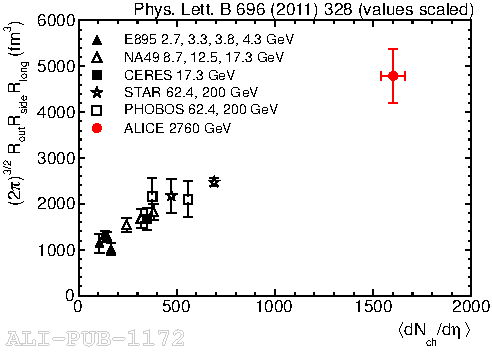
\includegraphics[width=0.5\textwidth]{ksfigures/HBTVolumeVsDensity.pdf}
\caption{Homogeneity volume for $k_{\rm T} = 0.3$~GeV as a function of the charged-particle density, measured in heavy-ion collisions at different energies. Adapted from~\cite{Aamodt:2011mr}.}
\label{figks:HBTvolume}
\end{figure}

The energy dependence of the HBT radii is usually expressed as a function of the cubic root of the charged-particle pseudorapidity density, i.e. as $({\rm d}N_{\rm ch}/{\rm d}\eta)^{1/3}$. The approximately linear increase (at a given $k_{\rm T}$) is well-described by hydrodynamical calculations~\cite{Chojnacki:2007rq,Karpenko:2009wf}. The product of the three radii, measured at different energies at $k_{\rm T} = 0.3$~GeV, is shown in Fig.~\ref{figks:HBTvolume} as a function of the charged-particle pseudorapidity density ${\rm d}N_{\rm ch}/{\rm d}\eta$. This product, multiplied by a factor $(2\pi)^{3/2}$ due to Gaussian distribution normalization, representing then the homogeneity volume, increases linearly with the particle density. At the LHC the homogeneity volume for pion emission for the 5\,\% most central Pb--Pb collisions doubles compared to that at the top RHIC energy. Within a hydrodynamic scenario the decoupling time for hadrons ($\tau_{\rm f}$, corresponding to kinetic freeze-out) can be extracted from the $k_{\rm T}$ dependence of $R_{\rm long}$ ($\tau_{\rm f} \propto R_{\rm long}$)~\cite{Herrmann:1994rr}. The decoupling time, estimated this way for different collision energies, is presented in Fig.~\ref{figks:HBTtime}. It increases linearly with $({\rm d}N_{\rm ch}/{\rm d}\eta)^{1/3}$, and reaches for most central LHC collisions a value by a factor 1.4 larger than was observed at RHIC. Note that the estimate for $\tau_{\rm f}$ was done for an assumed kinetic freeze-out temperature $T_{\rm kin} \approx 120$~MeV, if one were to use the latest measured value (Sec.~\ref{subsecks:identspectra}), the decoupling time would increase to 13--14~fm.

\begin{figure}
\centering
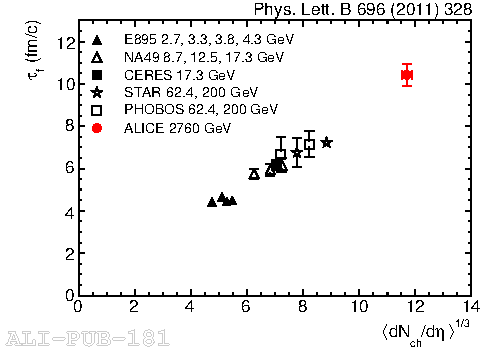
\includegraphics[width=0.5\textwidth]{ksfigures/HBTDecouplTime.pdf}
\caption{Decoupling time as a function of the cube root of charged-particle pseudorapidity density, measured in heavy-ion collisions at different energies. Reproduced from~\cite{Aamodt:2011mr}.}
\label{figks:HBTtime}
\end{figure}

In the study of two-pion correlations, the assumption was that the pion emission is incoherent, i.e. the source is fully chaotic. In such conditions the strength of the Bose--Einstein correlations is maximal, and would decrease for a source with a lower degree of chaoticity. Such a situation may be created in heavy-ion collisions, if some kind of condensate would be present or formed (e.g. colour-glass condensate, disoriented chiral condensate). The degree of chaoticity can be assessed comparing two- and three-pion correlations. A recent analysis~\cite{Abelev:2013pqa} found that the genuine three-pion correlation is suppressed relative to the two-pion correlation, assuming fully chaotic pion emission. This suppression decreases with pion-triplet momentum, and at low momentum (pion $p_{\rm T} \sim 0.3$~GeV) may correspond to a coherent fraction in charged pion emission of $(22 \pm 12)$\,\%.


%HBT sizes vs particle density
%volume vs energy
\subsection{Fluctuations}
\label{subsecks:fluct}
Study of event-by-event fluctuations provides a tool to characterize the thermodynamic properties of the system. Such fluctuations are also affected by the system evolution. The fluctuations of conserved quantities in a finite phase space window, such as the net charge of the system described in~\cite{Abelev:2012pv}, are predicted to be sensitive signals of QGP formation and of the phase transition and may provide an important insight on the properties of strong interactions. In the QGP phase, the charge carriers are quarks with their fractional charges, whereas particles in the hadron phase carry unit charge. The fluctuations in the net charge depend on the squares of the charge states present in the system. Consequently, the net-charge fluctuations in the QGP phase are expected to be significantly smaller compared to those in the hadron phase. The event-by event fluctuations of the net charge in a specific phase-space window (for example a given pseudorapidity interval around mid-rapidity) are usually quantified by the $D$ variable~\cite{Jeon:2000wg}, defined as:
\begin{equation}
D = \langle N_{+} + N_{-} \rangle \langle \delta (N_{+} / N_{-})^2 \rangle \approx 4 \langle \delta (N_{+} - N_{-})^2 \rangle / \langle N_{+} + N_{-} \rangle .
\end{equation}
Here $N_{+,-}$ are the numbers of particles of the two charges in that window, angle brackets denote the average value over the ensemble of events, and $\delta$ indicates the variance of the quantity under the square sign. The value of $D$ measures the fluctuation of the net charge ($N_{+} + N_{-}$) per entropy unit, and is predicted to be around 3 for hadron gas and significantly lower, 1--1.5, for the QGP phase~\cite{Jeon:2003gk}. Figure~\ref{figks:ChargeFluct} presents the energy dependence of the D measure obtained by the STAR experiment~\cite{Abelev:2008jg} at RHIC and by ALICE at the LHC in the most central collisions. The fluctuations are expected to be diluted during the medium evolution and thus the D measure may not reach the value predicted for the QGP phase, however, a clear tendency going closer to that prediction with increasing energy is observed.

\begin{figure}
\centering
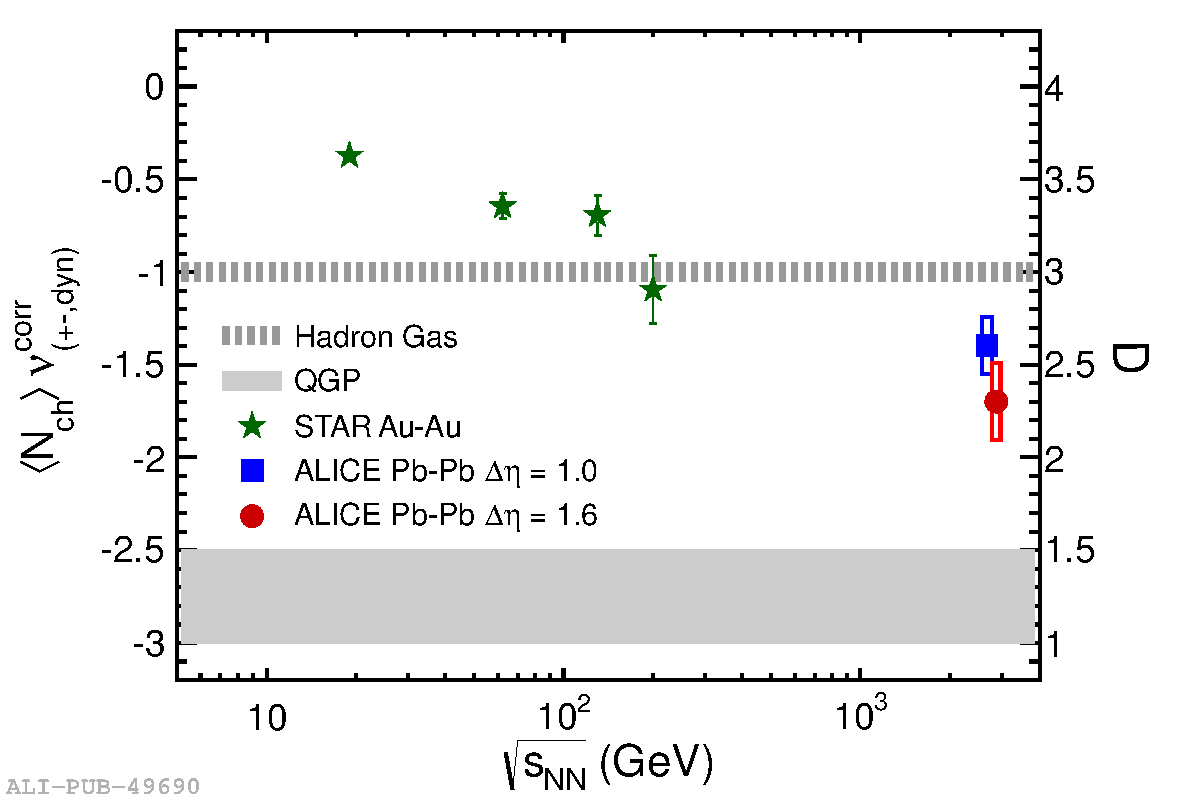
\includegraphics[width=0.5\textwidth]{ksfigures/NetChargeFluct.pdf}
\caption{Energy dependence of net-charge fluctuations represented as D-measure (defined in the text) in the most central collisions. The two ALICE measurements are for two different pseudorapidity intervals $\Delta\eta$ centred around mid-rapidity, and the STAR results are for $\Delta\eta = 1$. The D values are shown on the right-hand ordinate and the shaded areas correspond to the two predictions according the legend. The quantity of the left-hand side ordinate represents the way how the D values are measured, and it is not discussed here. Reproduced from~\cite{Abelev:2012pv}.}
\label{figks:ChargeFluct}
\end{figure}

Event-by-event fluctuations of the mean transverse momentum of charged particles are studied as a function of the charged-particle multiplicity in Pb--Pb collisions with the ALICE experiment, and significant non-statistical fluctuations are observed. The dynamical mean $p_{\rm T}$ fluctuations arise from correlations among the $p_{\rm T}$ of the final-state particles, e.g. due to resonance decays, jets, or quantum correlations. To account for such conventional contributions, similar studies are performed in pp, where these correlations are also present.  These fluctuations are expected to decrease with increasing particle density (collision centrality), as $({\rm d}N_{\rm ch}/{\rm d}\eta)^{-1/2}$ under the assumption of independent sources. The measured dependence for peripheral collisions (corresponding to centrality percentiles in the range 60--90\,\%) follows the pp extrapolation, however, already there the particle-density dependence has a power close to $-0.4$ instead of $-1/2$. This is interesting, because significant differences in the mean $p_{\rm T}$ are observed between pp and Pb--Pb in that multiplicity range~\cite{Abelev:2013bla}. At larger particle densities the Pb--Pb fluctuation results deviate from the pp extrapolation: an enhancement in the 40--60\,\% centrality range is followed by a pronounced decrease for more central events, which indicates a strong reduction of fluctuations towards central collisions. This centrality dependence is compatible with that observed at RHIC~\cite{Adams:2005ka}. The Pb--Pb data can not be described by models based on independent nucleon--nucleon collisions such as HIJING~\cite{Wang:1991hta,Deng:2010xg}. Models which include initial state density fluctuations and their effect on the development of collectivity in the final state such as AMPT~\cite{Lin:2004en} are in reasonable qualitative agreement with the data. This suggests a connection between the observed transverse momentum fluctuations and azimuthal correlations, and their relation to fluctuations in the initial state of the collision.

%charge particle balance function
\subsection{Angular correlations}
\label{subsecks:angular}
The angular correlations between two particles are widely used to study various phenomena of both non-flow and collective-flow origin. Here, the method and some applications to non-flow studies is described. The exploitation of the angular correlations for investigation of the azimuthally-dependent flow is explained in Sec.~\ref{sec:ps:flow}. The two-particle correlation between pairs of particles is measured as a function of the azimuthal difference $\Delta\varphi$ (defined usually within $−\pi/2$ and $3\pi/2$) and pseudorapidity difference $\Delta\eta$. Various kinds of particle pairs are used: they can be all charged particles, pairs selected by charge (like sign, unlike sign), pairs when one particle (trigger) has given $p_{\rm T}$ or type while the second particle (associated) may have some other characteristics, etc. The two-dimensional distribution is constructed for pairs of particles from the same event, and basically two types of the normalization are used: each event is normalized (per number of pairs, or number of triggers) and then the events are summed up, or the events are first summed up and then normalized to the total number (of pairs or triggers). Therefore, one has to be careful, when comparing the results from different experiments, which may have employed different normalization. Then a second two-dimensional distribution is constructed for pairs of particles from the different events (or a trigger particle form one event and all associated from another one). This mixed-event distribution is usually uniform in the $\Delta\varphi$ direction and has a triangular shape in the $\Delta\eta$ direction, reflecting the geometrical acceptance: maximum at $\Delta\eta = 0$, dropping to zero at $\Delta\eta = \pm$~the detector size in pseudorapidity. The second distribution is normalized to unity at its maximum (i.e. at $\Delta\eta = 0$), and then used to divide the normalized distribution obtained for particle pairs from the same event. In this way, the acceptance and detection efficiency are taken into account.

\begin{figure}
\centering
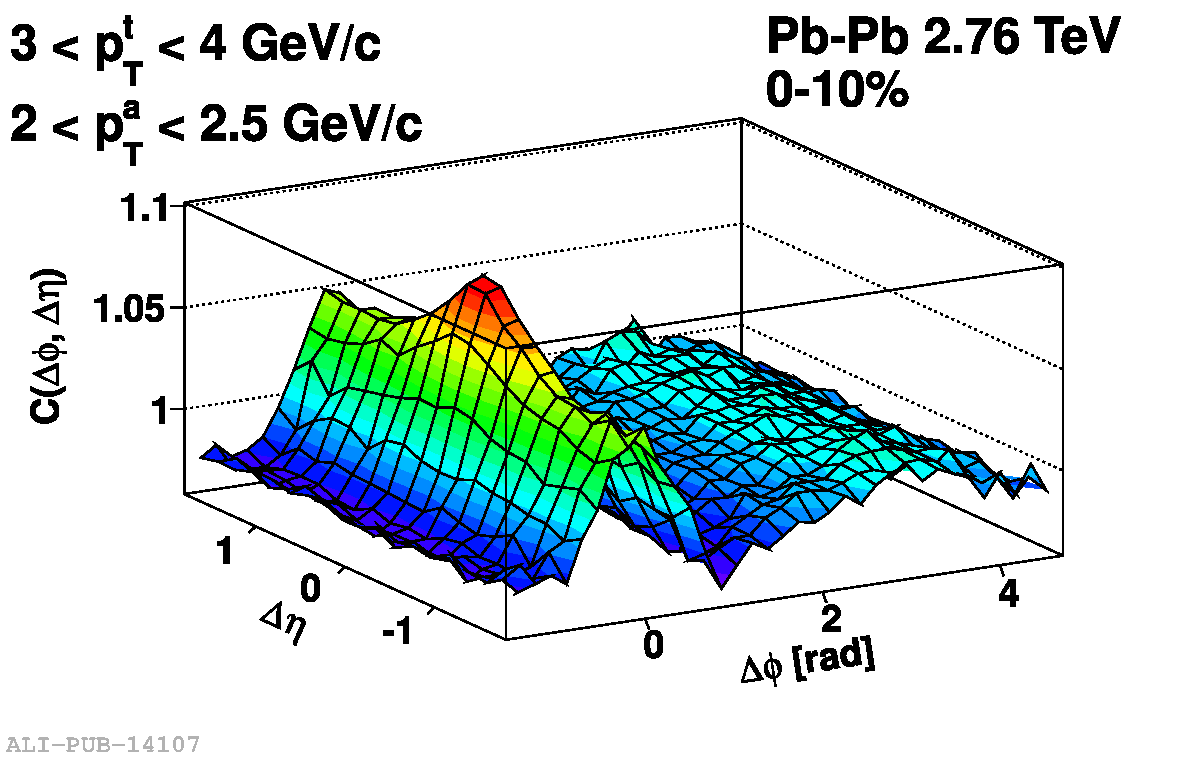
\includegraphics[width=0.5\textwidth]{ksfigures/TwoParticleCorrFunction.pdf}
\caption{Example of the two-particle correlation function in $\Delta\varphi$ and $\Delta\eta$ for trigger and associated particle selected in $p_{\rm T}$ intervals displayed in the upper-left corner. The top 10\,\% of most central Pb--Pb collisions are used. Reproduced from~\cite{Aamodt:2011by}.}
\label{figks:CorrExamle}
\end{figure}


An example of such two-dimensional two-particle particle correlation is illustrated in Fig.~\ref{figks:CorrExamle}. This is obtained for trigger--associated particle pairs selected according their $p_{\rm T}$ as indicated in the figure. Some typical structures are apparent:
\begin{itemize}
 \item{the peak around $(\Delta\varphi,\Delta\eta) = (0,0)$ is due to (mini-)jets, sometimes a much narrower peak is also visible on top of that, caused by HBT correlations (for like-sign pairs), or by gamma conversions (for unlike-sign pairs);}
 \item{the near-side ridge at $\Delta\varphi = 0$ continuing from the jet peak along the $\Delta\eta$ direction to larger $\Delta\eta$ values, this is presumably caused by the elliptic and higher-harmonic flow (see Sec.~\ref{sec:ps:flow};}
 \item{the away-side ridge at $\Delta\varphi = \pi$ along the $\Delta\eta$ direction, where the second jet may appear (often quenched), now spread along $\Delta\eta$ because the parton--parton system at the origin of the two jets moves longitudinally with respect to the collision centre-of-mass system, in addition the flow azimuthal modulation also contributes here.}
\end{itemize}
The angular two-particle correlations are analyzed by studying their centrality development, and often by projecting them on one of the axes, excluding or not some structures discussed above.

The two-particle correlations are used to study parton quenching at $p_{\rm T}$ below ${\cal O}(10)$~GeV~\cite{Aamodt:2011vg}, where the full jet reconstruction is difficult due to background fluctuations~\cite{Abelev:2012ej}. In the example shown here the selection requires: a trigger within $8 < p_{\rm T}^{\rm t} < 15$~GeV while the associated $p_{\rm T}^{\rm a}$ is a variable parameter, respecting $p_{\rm T}^{\rm a} <p_{\rm T}^{\rm t}$. The two-dimensional correlation is projected on the $\Delta\varphi$ axis in order to measure the number of associated particles correlated to the trigger particle in the near-side and the away-side jet structures. The background from the underlying event, possibly modulated by elliptic flow, has to be subtracted. This is done using three methods: a flat background obtained by the ZYAM (Zero Yield At Minimum) method (the minimum between the near- and the away-side peaks is used to evaluate the background level), a background modulated according the available elliptic-flow $v_2$ measurements, and a flat background estimated according to the value in the region $|\Delta\varphi| < \pi/2$ and $|\Delta\eta| > 1$  ($\Delta\eta$-gap). After background subtraction the distribution is integrated around the near- and away-side peaks, in the $\pm 0.7$ and $\pi \pm 0.7$ $\Delta\varphi$ intervals, respectively. The per-trigger yields of associated particles, obtained this way, are normalized to the same yields measured in pp collisions. Such a ratio is denoted $I_{\rm AA}$ and it represents the nuclear modification factor of the conditional yields. In Fig.~\ref{figks:IAA} the near- and away-side $I_{\rm AA}$ are presented as a function of associated-particle $p_{\rm T}^{\rm a}$ for peripheral and central Pb--Pb collisions. The results are practically independent on $p_{\rm T}^{\rm a}$, and for peripheral collisions compatible with unity, i.e. no nuclear modification is observed. For central collisions, the away-side $I_{\rm AA}$ is around 0.6, which is interpreted as a manifestation of jet quenching. On the near-side the $I_{\rm AA}$ is above unity, such an effect was not observed at lower energies. The near-side enhancement could be understood as due to a modification of the fragmentation function, possibly caused by jet quenching and a trigger bias. This measurement constrains various models, some of those showed to be capable to describe such an enhancement~\cite{Renk:2011wp}.

\begin{figure}
\centering
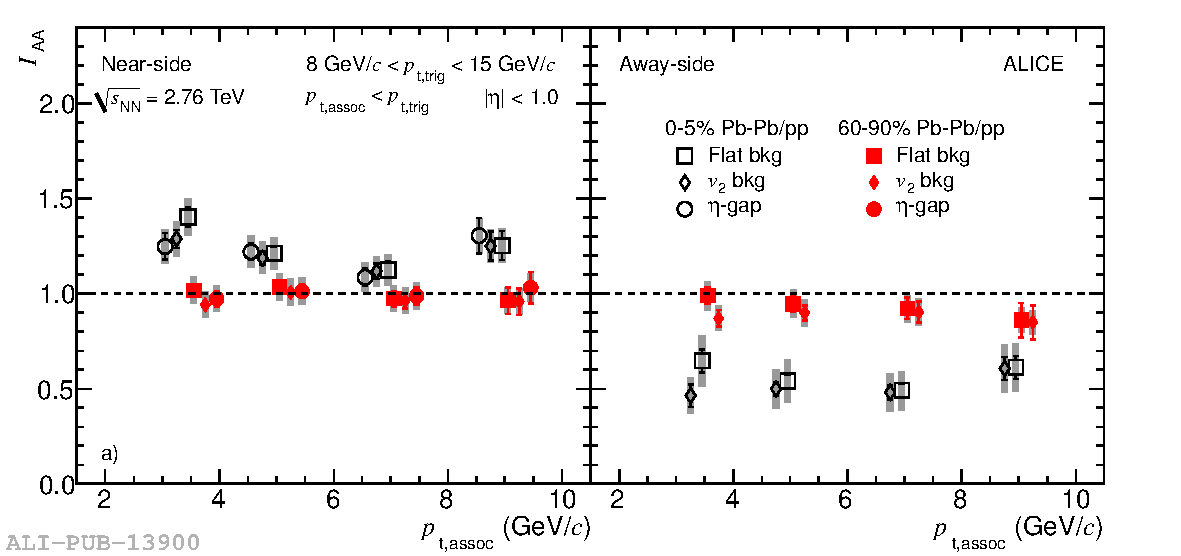
\includegraphics[width=0.7\textwidth]{ksfigures/IAA.pdf}
\caption{Near-side (left) and away-side (right) $I_{\rm AA}$ as a function of the transverse momentum of associated particles. The results are shown for peripheral (60--90\,\%) and central (0--5\,\%) Pb--Pb collisions. The three values shown for each measurement correspond to the three background subtraction methods described in the text. Reproduced from~\cite{Aamodt:2011vg}.}
\label{figks:IAA}
\end{figure}

The jet-shape studies measuring the jet-structure widths in $\Delta\varphi$ and $\Delta\eta$ directions, exploited the triggered two-particle correlations as well. It was reported that the $\Delta\eta$ jet-structure size increases for more central Pb--Pb collisions, while in the $\Delta\varphi$ direction such an increase, if any, is much smaller. This could be explained by an interaction of the jet with longitudinally flowing medium. The particle composition of the jet-like structure was also studied. The p/$\pi$ ratio is measured in $(\Delta\varphi, \Delta\eta)$ regions, both outside and inside the jet structures selected in the correlation plot. Correcting the jet region with properly weighted outside-jet measurement, the p/$\pi$ ratio for the jet structure is obtained. While the outside-jet p/$\pi$ ratio reproduces the heavy-ion baryon anomaly (see Sec.~\ref{subsecks:identspectra}), the result for the jet structure is compatible with the expectation for the jet fragmentation in pp collisions.

\begin{figure}[!ht]
\centering
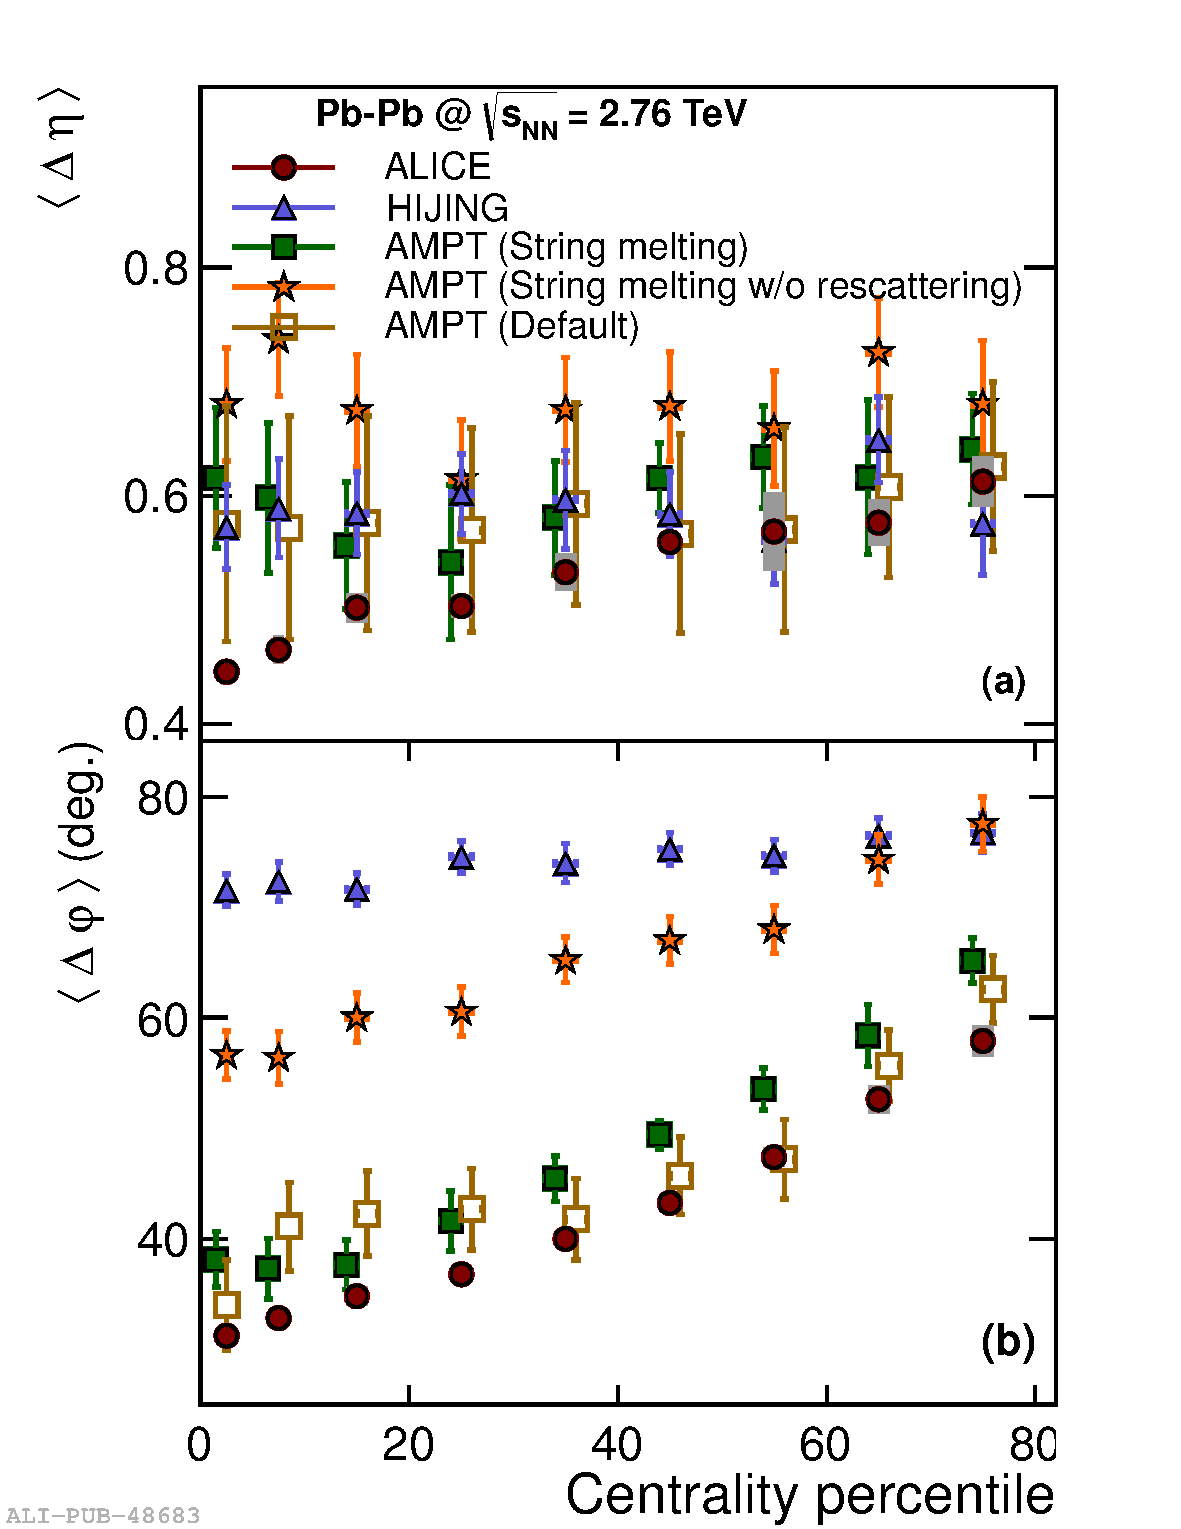
\includegraphics[width=0.5\textwidth]{ksfigures/BalanceFunctionWidth.pdf}
\caption{Charge balance function widths in longitudinal (upper part - a) and azimuthal (lower part - b) directions as a function of collision centrality, expressed in percentiles. Model calculations are presented with markers according to the legend. Reproduced from~\cite{Abelev:2013csa}.}
\label{figks:Balance}
\end{figure}

The study of the charge balance function is performed using the correlations constructed for unlike-sign and like-sign particle pairs separately~\cite{Abelev:2013csa}. The balance function is defined as one half of the difference between the unlike-sign and like-sign correlations, and measures the distance over which the charge of particles is compensated. The widths of the balance function in the two directions, $\langle \Delta\varphi \rangle$ and $\langle \Delta\eta \rangle$, are shown in Fig.~\ref{figks:Balance} as a function of the collision centrality. The measurement indicates that the charge is compensated in both directions on a shorter scale for more central collisions. Such behaviour was already observed at RHIC~\cite{Aggarwal:2010ya}, however, the $\langle \Delta\varphi \rangle$ and $\langle \Delta\eta \rangle$ values are significantly larger at the LHC. The model calculations~\cite{Wang:1991hta,Lin:2004en} presented in Fig.~\ref{figks:Balance} have difficulties to reproduce the centrality dependencies in both directions.

\subsection{Chiral magnetic effect}
\label{subsecks:chiral}
Under the influence of the strong magnetic field along the direction of the angular momentum generated by the colliding nuclei, the quark spin alignment and the imbalance of the left- and right-handed quarks, would generate an electromagnetic current~\cite{Kharzeev:2004ey,Fukushima:2008xe,Kharzeev:2007jp}. Subsequent quark fragmentation into charged hadrons may induce a charge separation along the direction of the magnetic field (perpendicular to the reaction plane, defined by the beam axis and the centres of the colliding nuclei). This phenomenon is called the Chiral Magnetic Effect (CME). Azimuthal correlations among particles provide a powerful tool for the experimental study of particle production with respect to the reaction plane~\cite{Abelev:2012pa}.

Let's denote by $\psi_\pm$ the azimuthal angle of a particle of given charge with respect to the reaction plane. The orientation of the reaction plane itself is estimated by different techniques used in the studies of azimuthal asymmetry, Sec.~\ref{sec:ps:flow}. The multi-particle correlator $\langle \cos{(\psi_{\pm,\alpha} + \psi_{\pm,\beta})} \rangle$ (`multi-particle' because it depends on the reaction-plane angle, determined with other particles) probes the magnitude of the parity-odd amplitude possibly present in the azimuthal distribution with respect to the reaction plane~\cite{Voloshin:2004vk}. Such correlator also suppresses the background (non-flow) correlations unrelated to the reaction plane. It can be expressed as the difference of two terms: $\langle \cos{\psi_{\pm,\alpha}} \cos{\psi_{\pm,\beta}} \rangle$ and $\langle \sin{\psi_{\pm,\alpha}} \sin{\psi_{\pm,\beta}} \rangle$, the latter term quantifies the out-of-plane (i.e. in the direction of magnetic field) charge correlations sensitive to the CME. In order to evaluate the two terms separately, the two-particle correlator $\langle \cos{(\psi_{\pm,\alpha} - \psi_{\pm,\beta})} \rangle$ is used, which is independent of the reaction plane angle, however, susceptible to large background contributions. This second correlator is equal to the sum of the two terms mentioned above. It should be mentioned that both correlators could be affected by other effects, such as momentum conservation, local charge conservation, and fluctuations in the initial energy density.

\begin{figure}
\centering
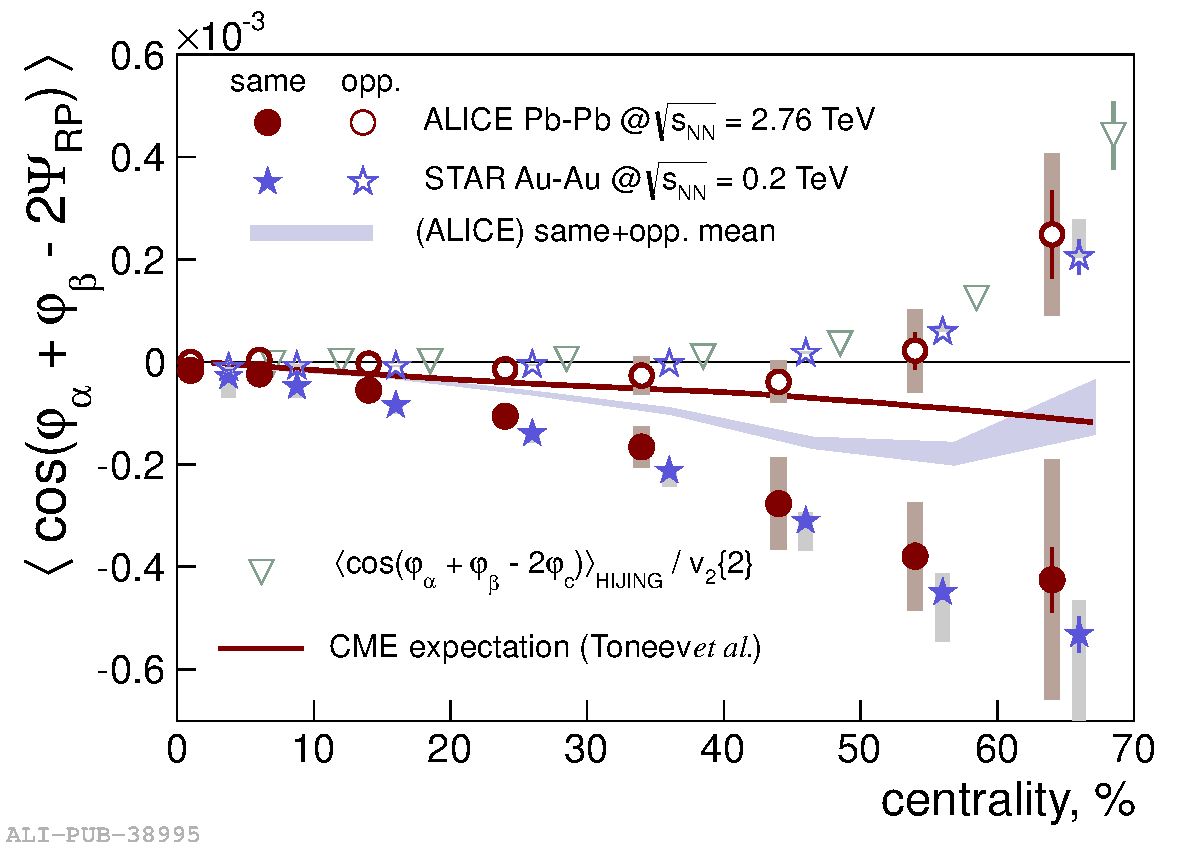
\includegraphics[width=0.5\textwidth]{ksfigures/ChargeSepar.pdf}
\caption{Centrality dependence of the multi-particle correlator defined in text as $\langle \cos{(\psi_{\pm,\alpha} + \psi_{\pm,\beta})} \rangle$. The ALICE results are obtained from the cumulant analysis.  The triangles represent the three-particle correlations from HIJING~\cite{Wang:1991hta} corrected for the experimentally measured $v_2$. A model prediction for the like-sign correlations incorporating the chiral magnetic effect for LHC energies~\cite{Toneev:2010xt} is shown by the solid line. The shaded band represents the centrality dependence of the charge independent correlations. Reproduced from~\cite{Abelev:2012pa}.}
\label{figks:ChSep}
\end{figure}


The centrality dependence of the multi-particle correlator $\langle \cos{(\psi_{\pm,\alpha} + \psi_{\pm,\beta})} \rangle$ for like-sign (labeled as `same') and unlike-sign (labeled as `opp.') particle pairs is presented in Fig.~\ref{figks:ChSep}. The contribution from the CME to the correlations of like-sign and unlike-sign pairs is expected to be similar in magnitude and opposite in sign, however, these correlations could be modified by the medium, that may result in the dilution of the correlations for unlike-sign particles. The LHC results are (unexpectedly) compatible with the RHIC measurements~\cite{Abelev:2009ac}. This is not true for the second (two-particle) correlator, may be due to different background contributions. In Fig.~\ref{figks:ChSep} the experimental results are compared to a model prediction for like-sign correlations~\cite{Toneev:2010xt}, which predicts a significantly smaller effect at the LHC than at RHIC. The magnitude of the effect and its energy dependence crucially rely on the duration and time evolution of the magnetic field, which is at present a matter of intense discussions. To conclude, a clear signal compatible with a charge-dependent separation relative to the reaction plane is observed and can be used to constrain theoretical calculations.

\section{Flow correlations}
\label{sec:ps:flow}
%5. Flow Correlations & Flow & PID Flow (PS)
%- Geometric fluctuations and origin of v_n vs ecc_n (Glauber, v3)
%- non-PID flow (ALICE first results)
%- PID flow (ALICE v2 scaling)
%- 2PC (CMS v_n?)
%- Event plane (ATLAS EP)
%- Explaining the ridge (2PC from 3 experiments)
%- Flow fluctuations
%- Event plane correlations
%- Success of viscous hydro
%- Comparison with RHIC
%- Flow in p+Pb (ridge, double ridge, PID)
%- Open questions

While the previous section covered physical mechanisms which induce
correlations between multiple hadrons, this section covers the
phenomenon of ``collective flow'', which leads to the correlations of
essentially all the particles in every event.
This results from the translation of anisotropies in the initial shape of the
colliding nuclei into anisotropies in momentum space, something that
would not occur if individual nucleon-nucleon collisions emitted independently
of each other.
The characterization of a ``shape'' in a final state particle distribution
is typically performed using a Fourier decomposition of the azimuthual
angle distrbution of final state particles.
Of course, averaging over an ensemble of independent events would lead to
the observation of no net anisotropy.  Thus, the presence of harmonic
oscillations in the final state requires the estimation of an ``event plane''
from the particle themselves, with an axis that points in the direction of
the largest momentum flow.

While this phenomenon was observed decades ago in the collisions of large
nuclei at low energies, this was straightforward to understand as the
reinteraction of the initial baryons and the produced hadrons, which
would thermalize and evolve as a ``hadron gas''.  
However, its persistence at higher energies, particularly 
\begin{figure}[!htb]
\begin{center}
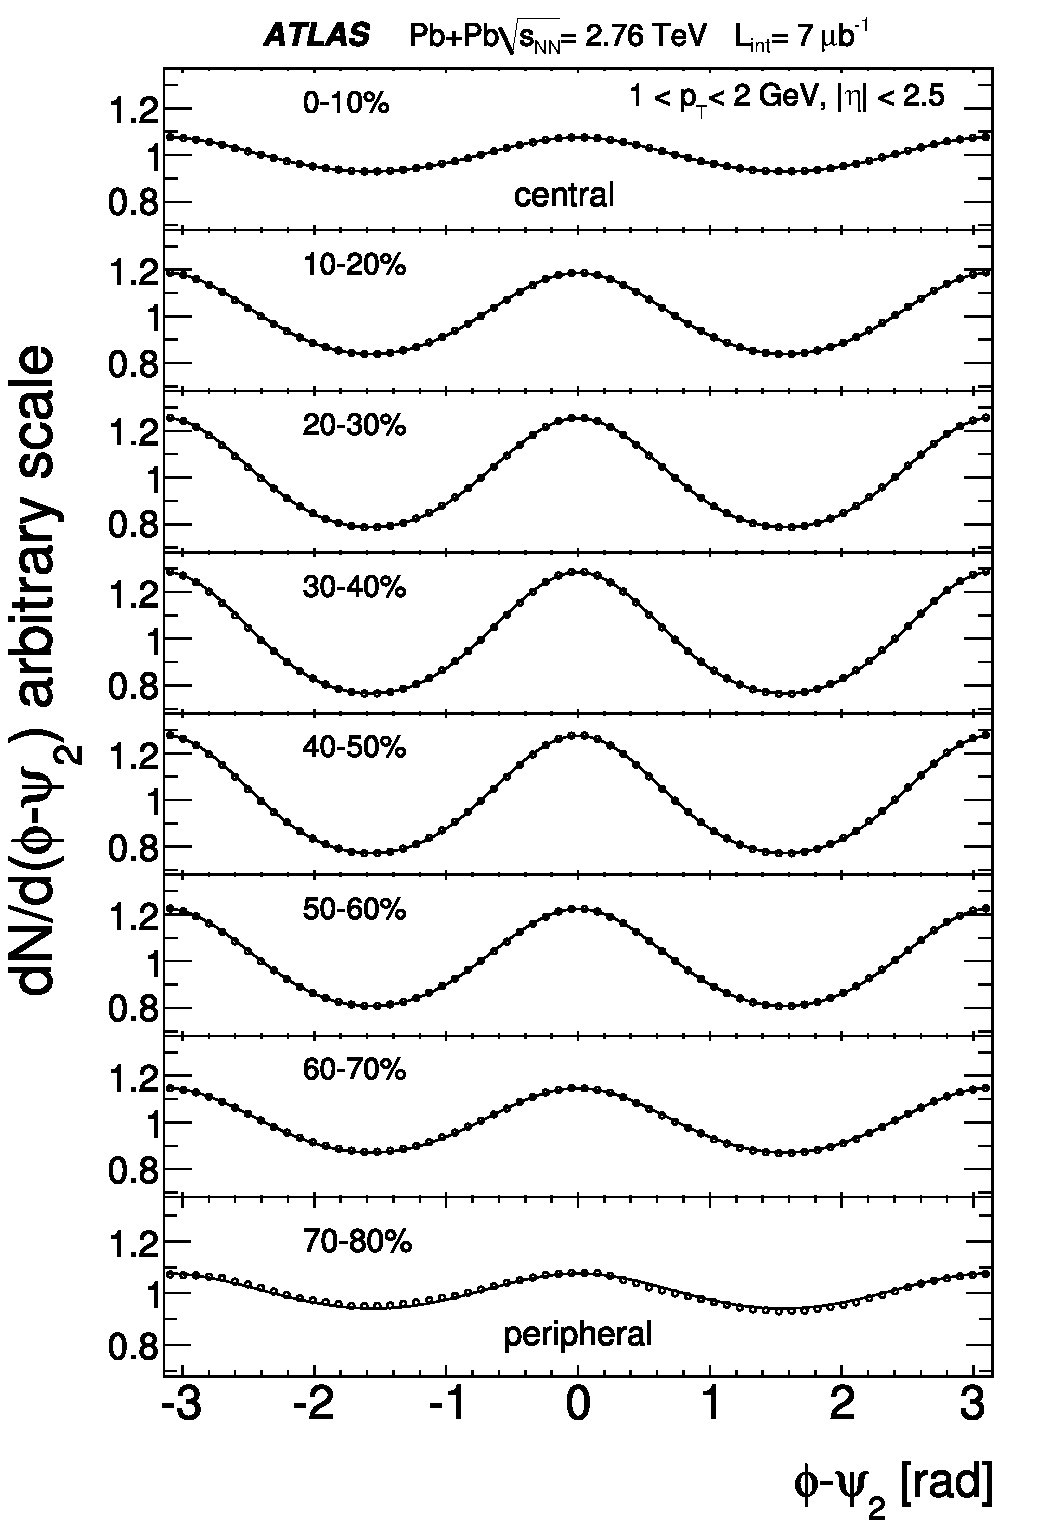
\includegraphics[width=0.49\textwidth]{flowcorrelations_figs/atlas_v2_fig_02.pdf}
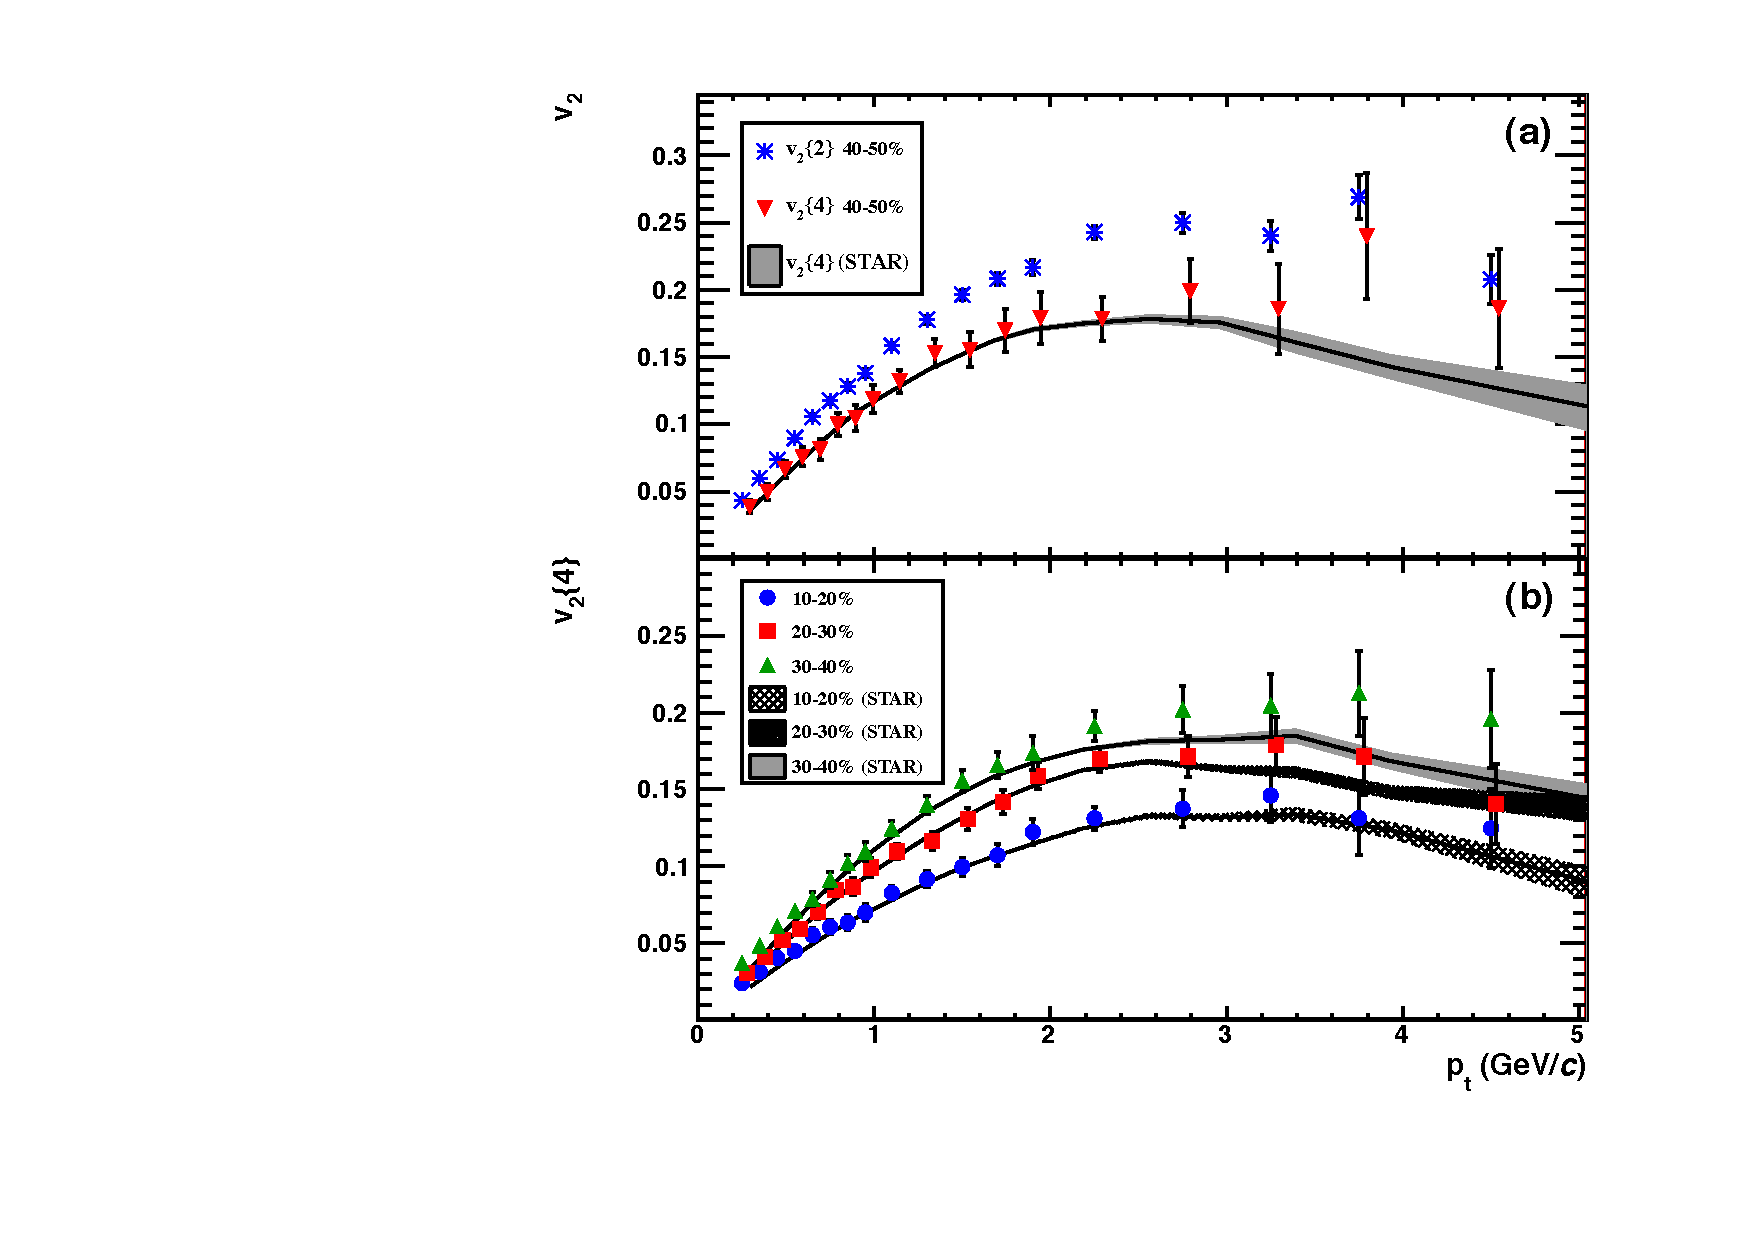
\includegraphics[width=0.49\textwidth]{flowcorrelations_figs/fig2.pdf}
\caption[]{(left) ATLAS data showing the evolution of anisotropy relative to the reaction plane, as a function of centrality (right) First ALICE data on \vtwo in Pb+Pb collisions at the LHC.}
\label{fig:pas:fc:firstreusults}
\end{center}
\end{figure}

\begin{figure}[!htb]
\begin{center}
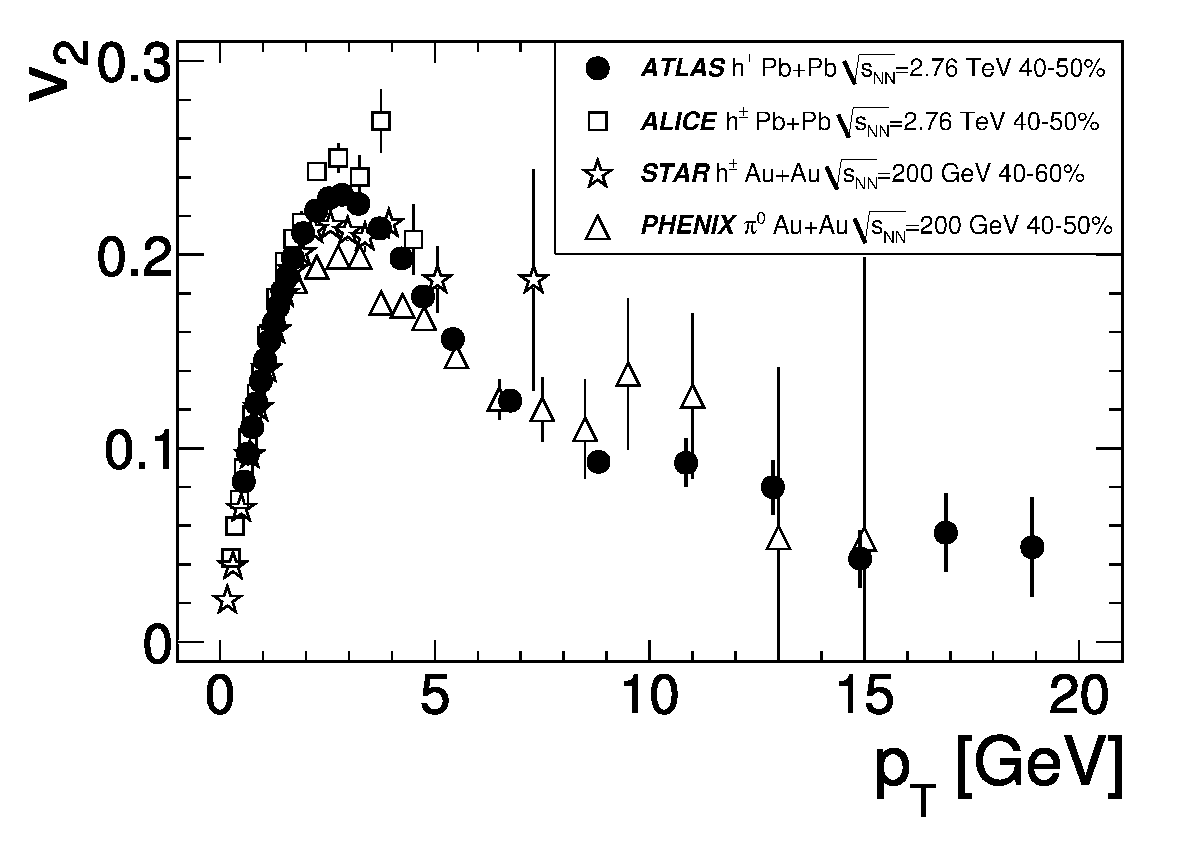
\includegraphics[width=0.49\textwidth]{flowcorrelations_figs/atlas_v2_fig_06.pdf}
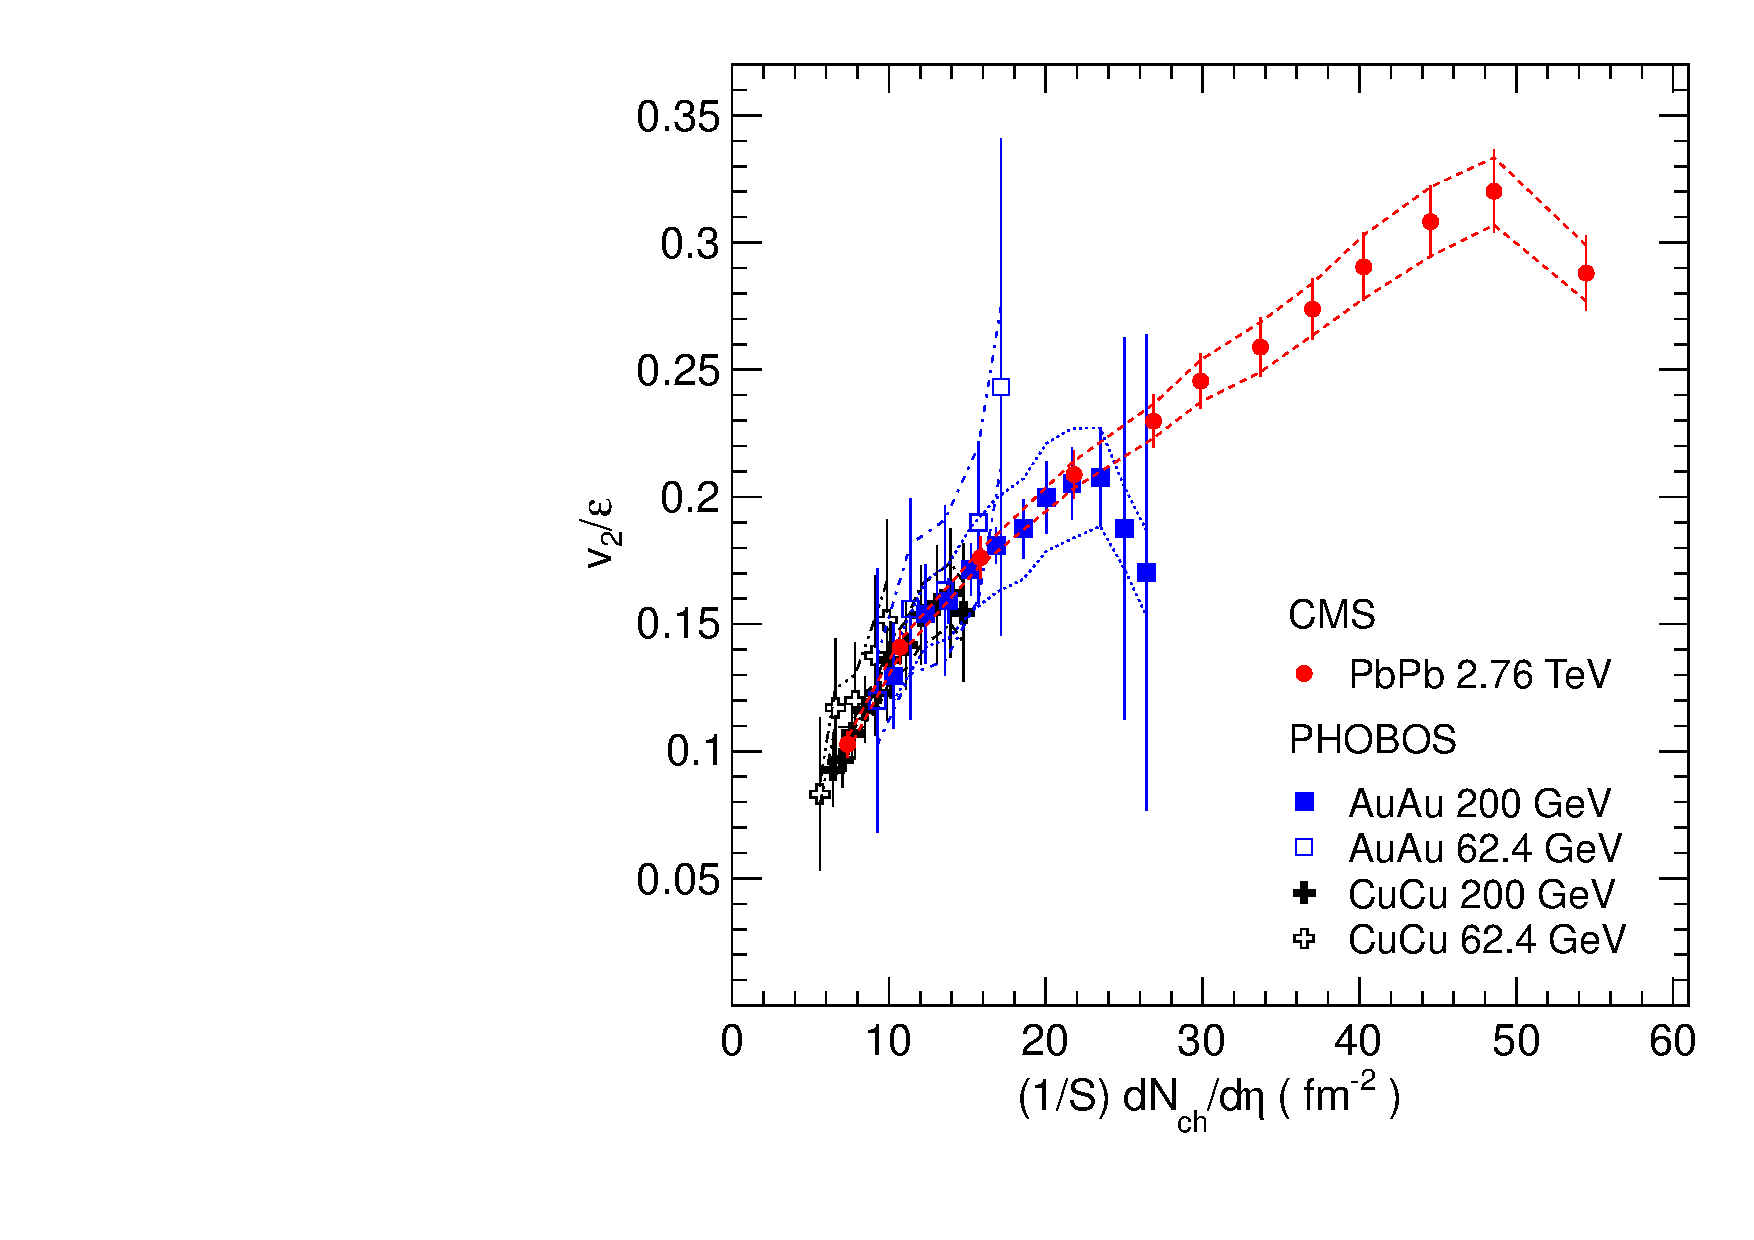
\includegraphics[width=0.49\textwidth]{flowcorrelations_figs/v2eps_dNdetaoverS_PHOBOS.pdf}
\caption[]{(left) ATLAS data showing the invariance of $\vtwo( \pT )$ with beam energy (right) CMS compilation showing the observed scaling of $\vtwo /\epsilon$ vs. $(1/S) dN_{ch}/d\eta$.}
\label{fig:pas:scaling}
\end{center}
\end{figure}

\begin{figure}[!htb]
\begin{center}
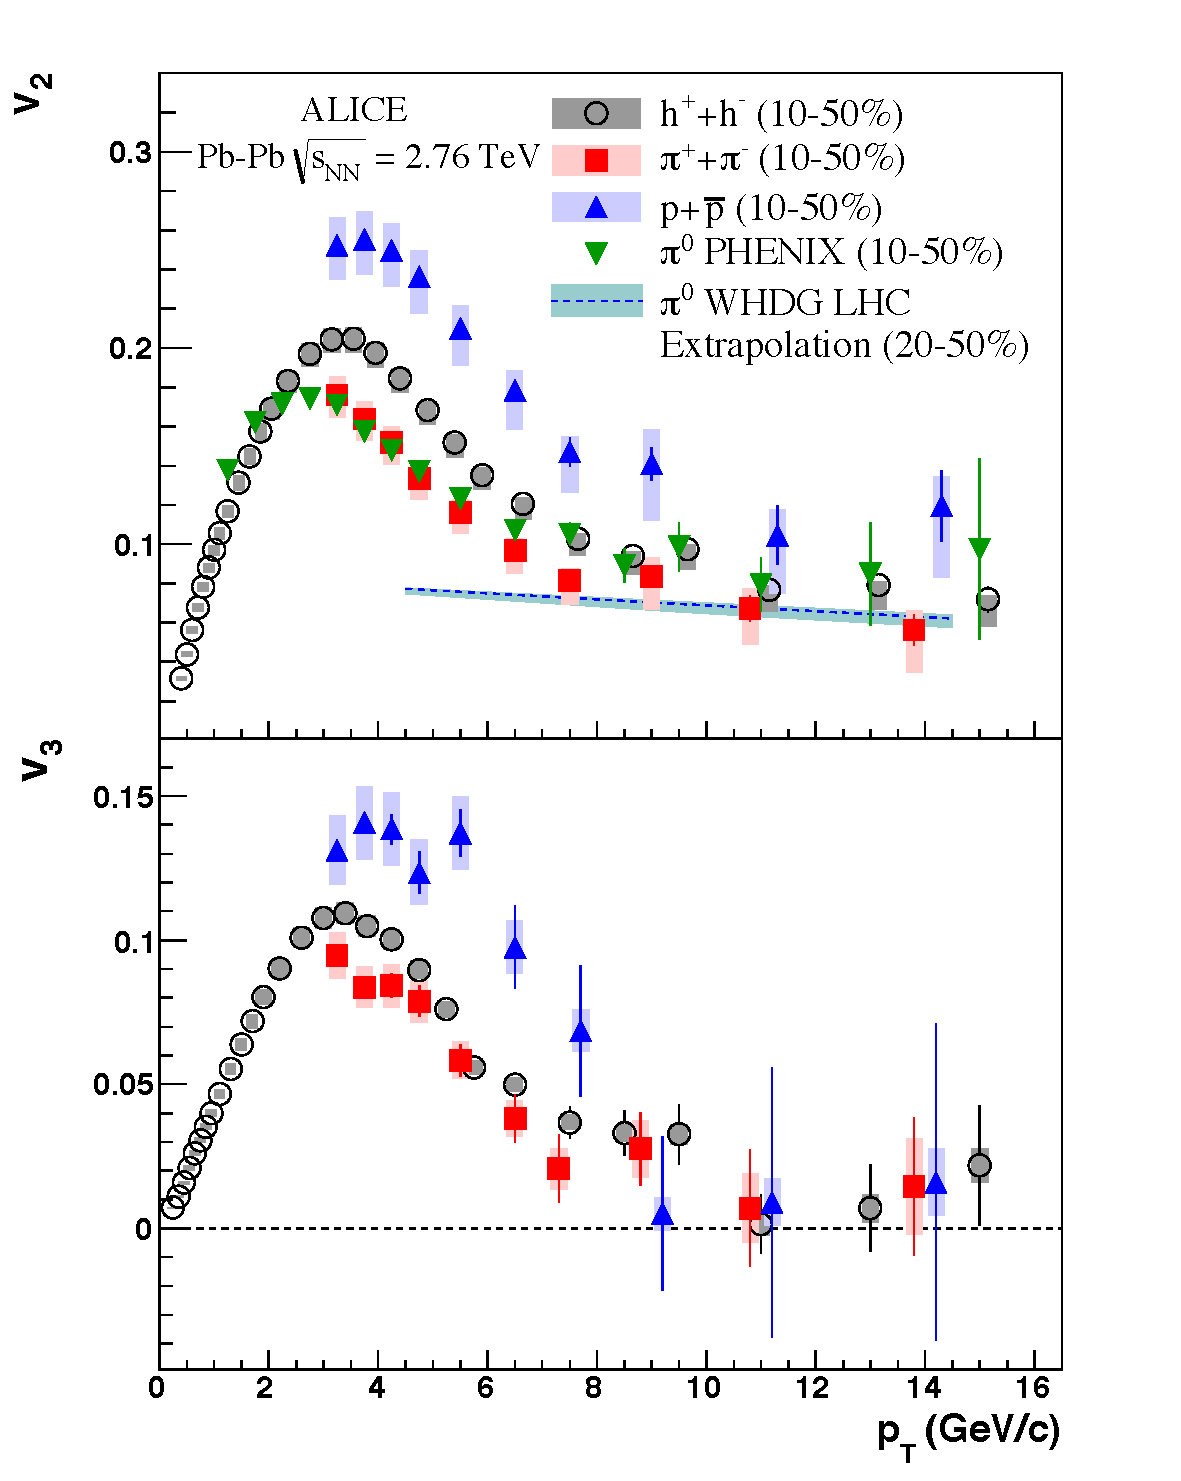
\includegraphics[width=0.49\textwidth]{flowcorrelations_figs/fig5_vn_pid.pdf}
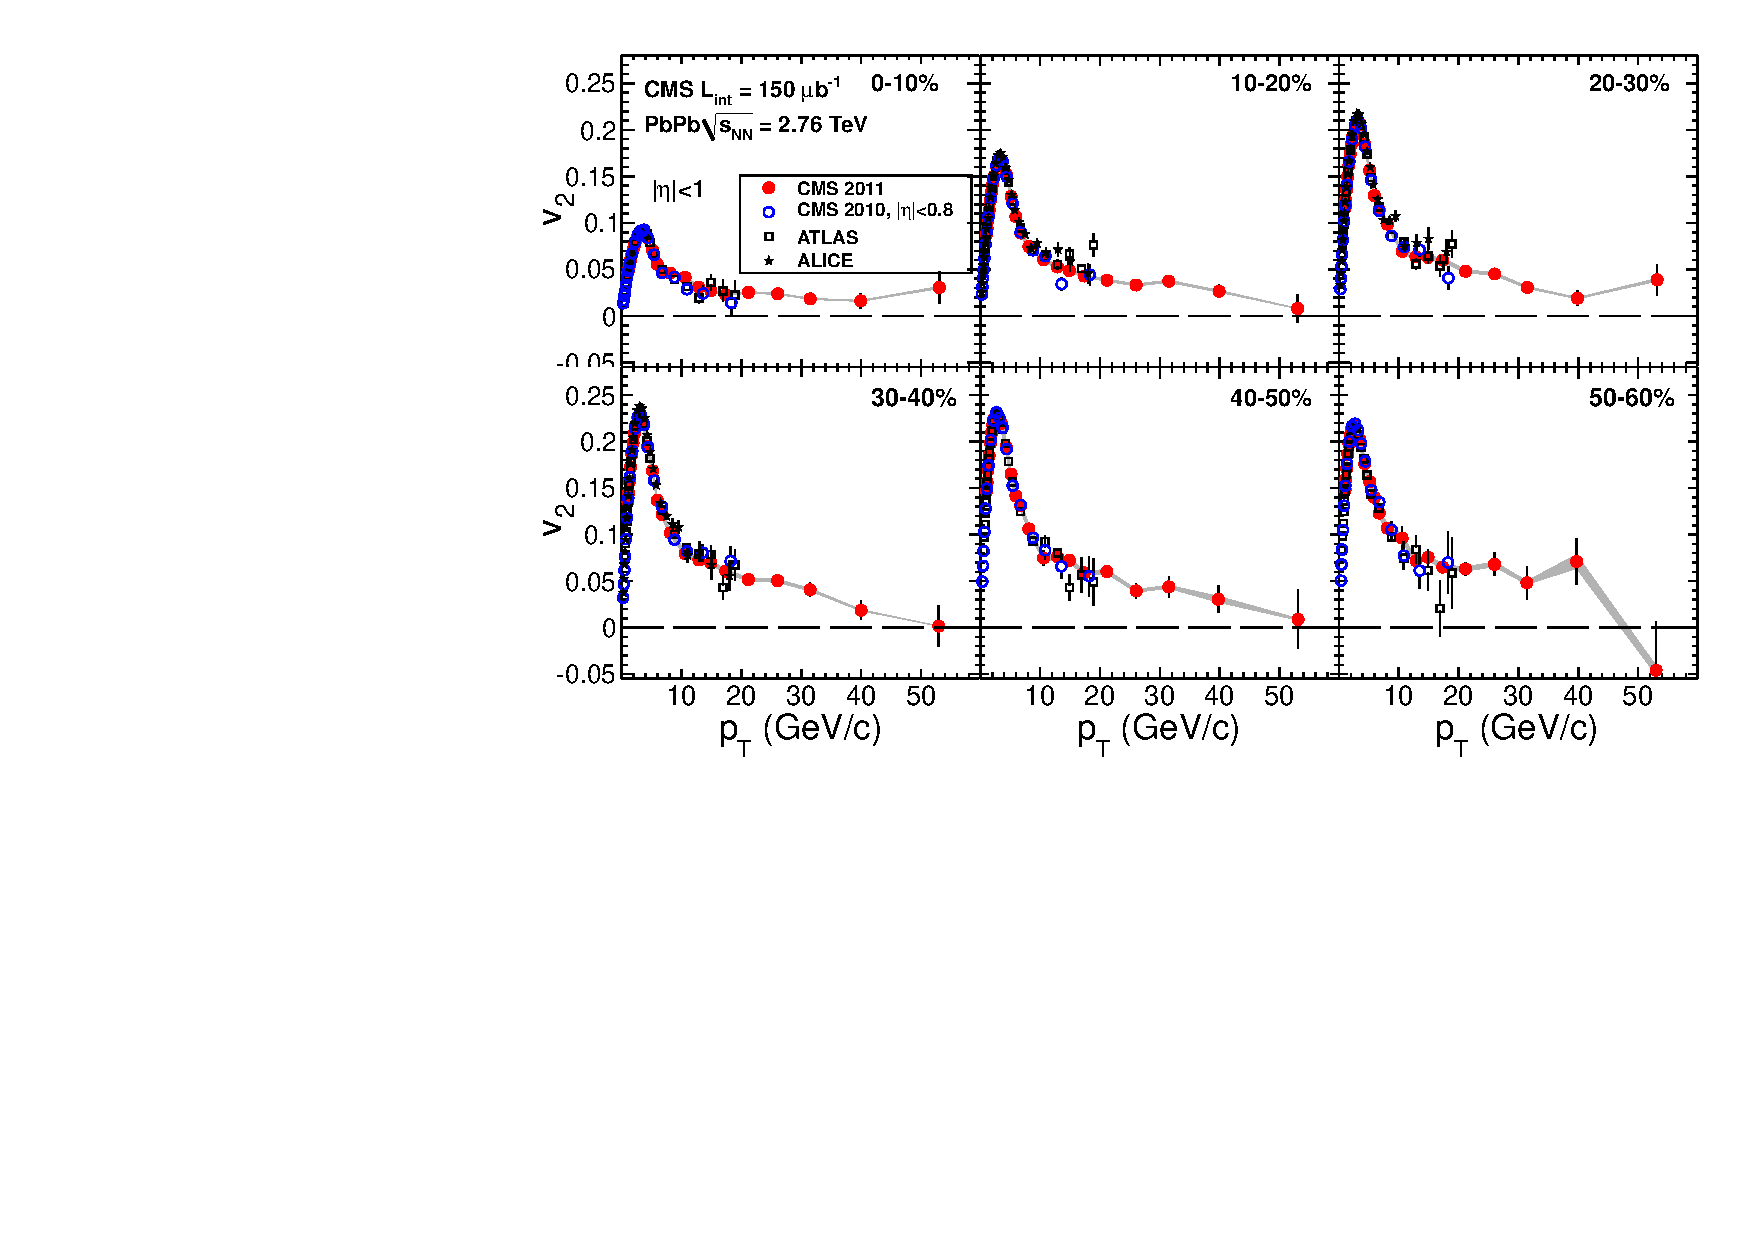
\includegraphics[width=0.49\textwidth]{flowcorrelations_figs/v2_pt_ep_atlas_alice_eta0-1_band_v5.pdf}
\caption[]{(left) ALICE data showing $\vtwo(\pT)$ for identified hadrons, for $|\eta|<0.8$ (right) CMS data showing the $\vtwo$ for unidentified hadrons at very high \pT, out to 50 GeV}
\label{fig:pas:fc:highpt}
\end{center}
\end{figure}

\begin{figure}[!htb]
\begin{center}
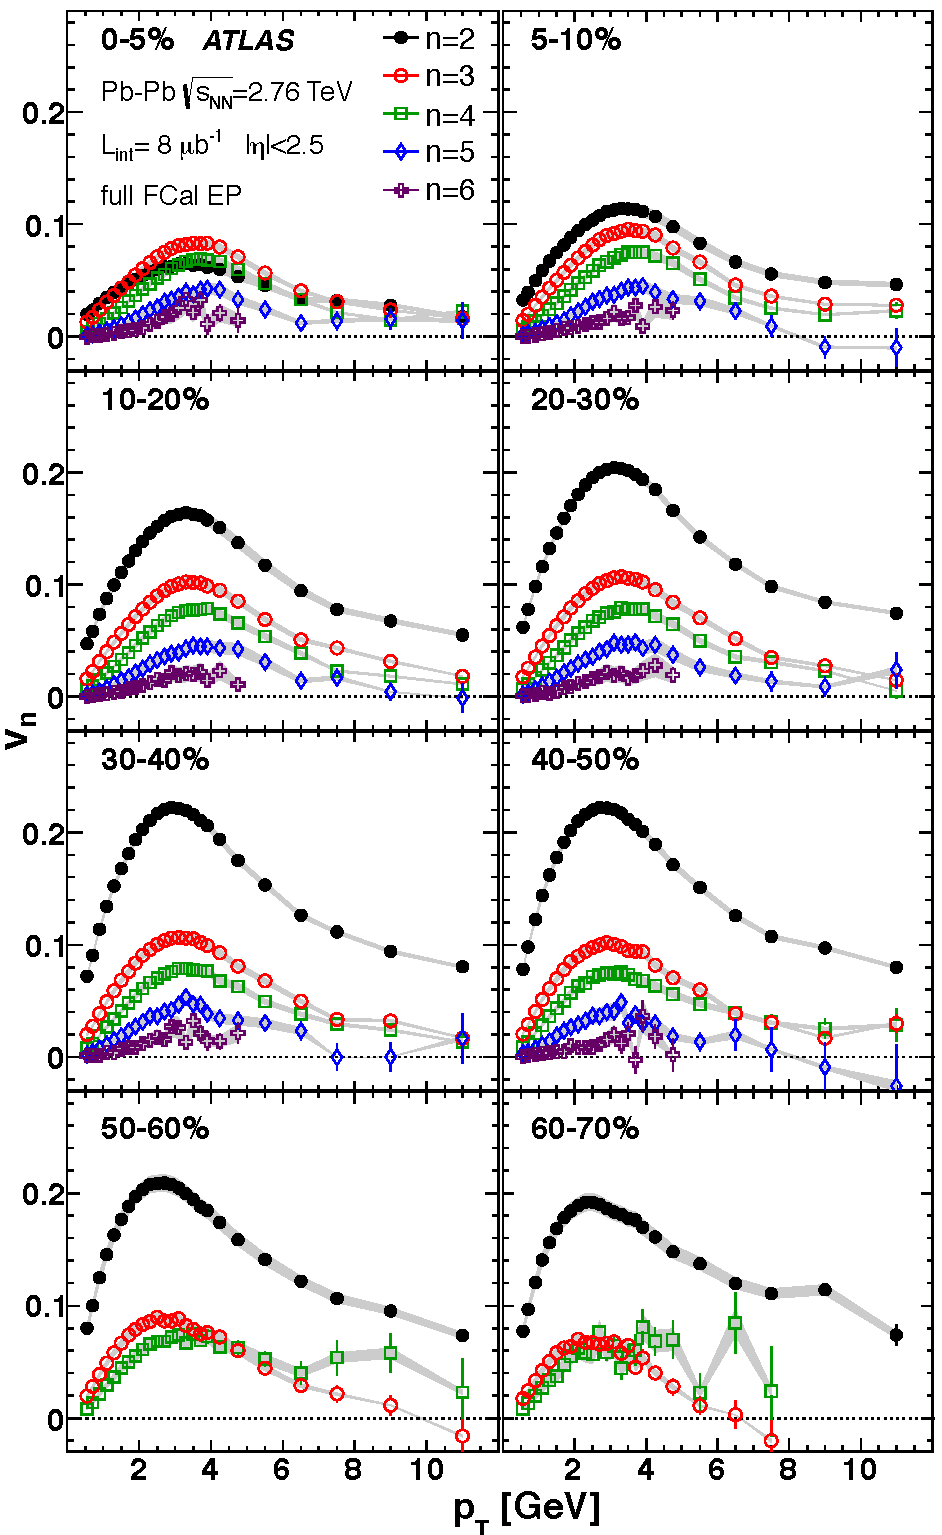
\includegraphics[width=0.49\textwidth]{flowcorrelations_figs/atlas_vn_fig_04.pdf}
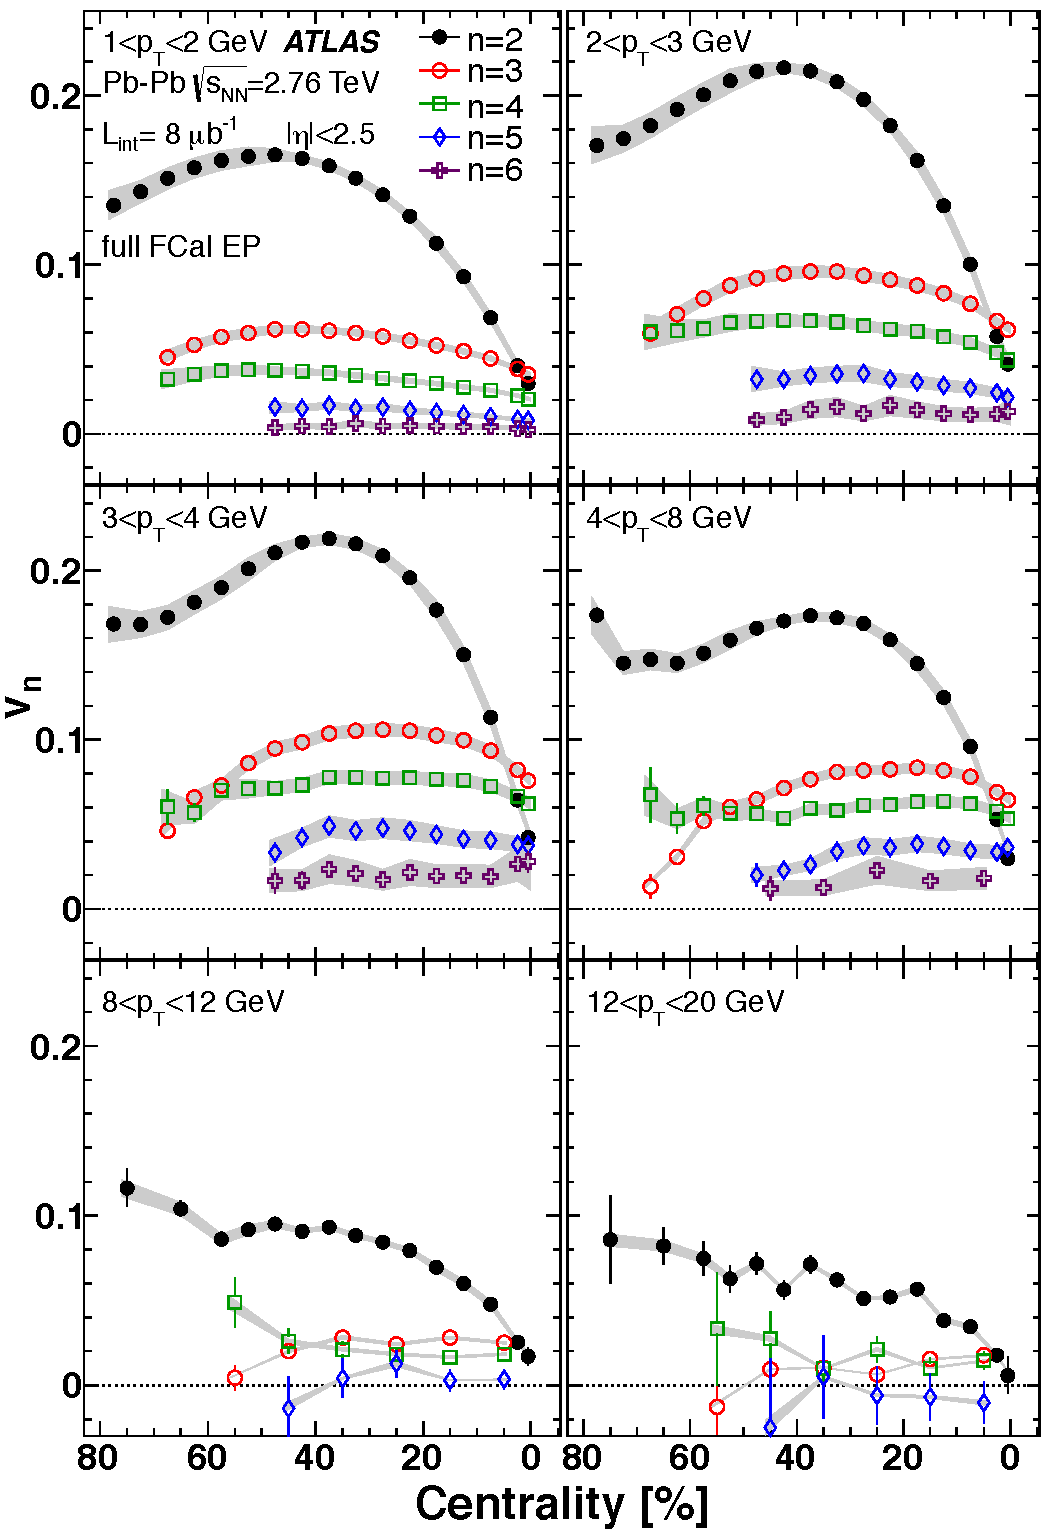
\includegraphics[width=0.49\textwidth]{flowcorrelations_figs/atlas_vn_fig_05.pdf}
\caption[]{(left) ATLAS data showing $v_n(\pT)$ for different centrality intervals and $|\eta|<2.5$, for $n=2-6$.  Very little dependence on $\eta$ is observed.  
(right) The same ATLAS data, in \pT intervals, showing the centrality dependence of $v_n$.}
\label{fig:pas:fc:vn}
\end{center}
\end{figure}

\begin{figure}[!htb]
\begin{center}
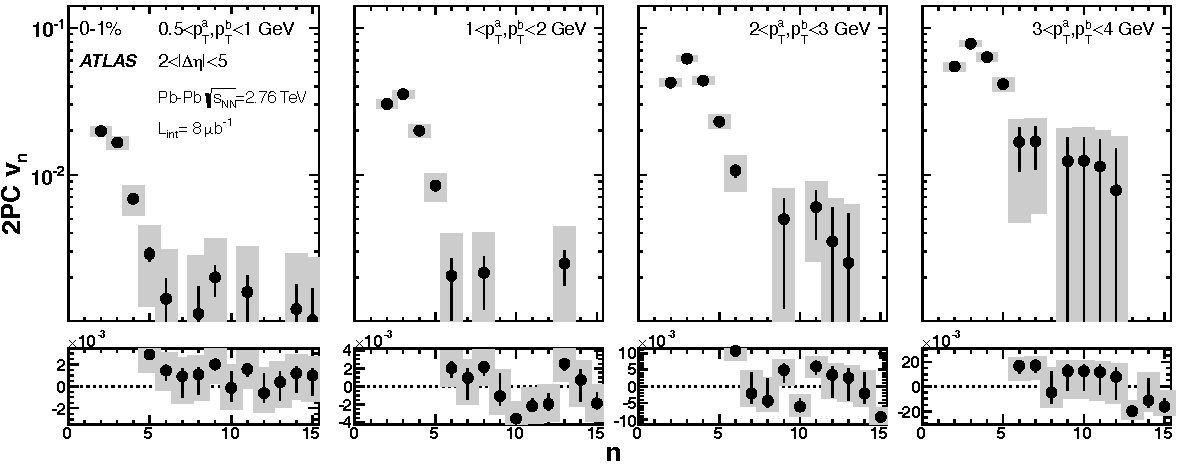
\includegraphics[width=0.98\textwidth]{flowcorrelations_figs/atlas_vn_fig_13.pdf}
\caption[]{
ATLAS data showing the $n$ dependence of $v_n$ in four \pT intervals, which are effectively
angular power spectra at different resolution scales.
}
\label{fig:pas:fc:powerspec}
\end{center}
\end{figure}

\begin{figure}[!htb]
\begin{center}
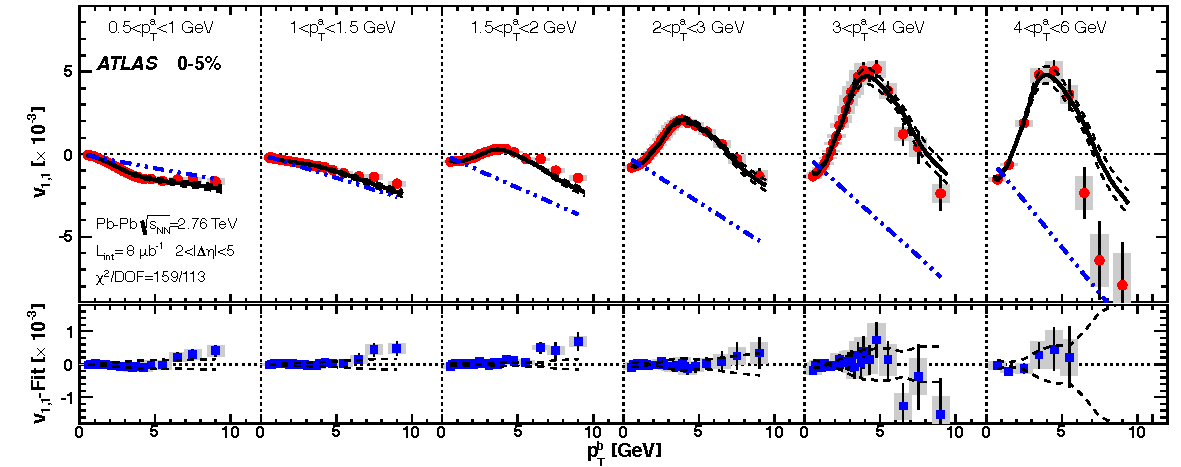
\includegraphics[width=0.98\textwidth]{flowcorrelations_figs/atlas_vn_fig_20a.pdf}
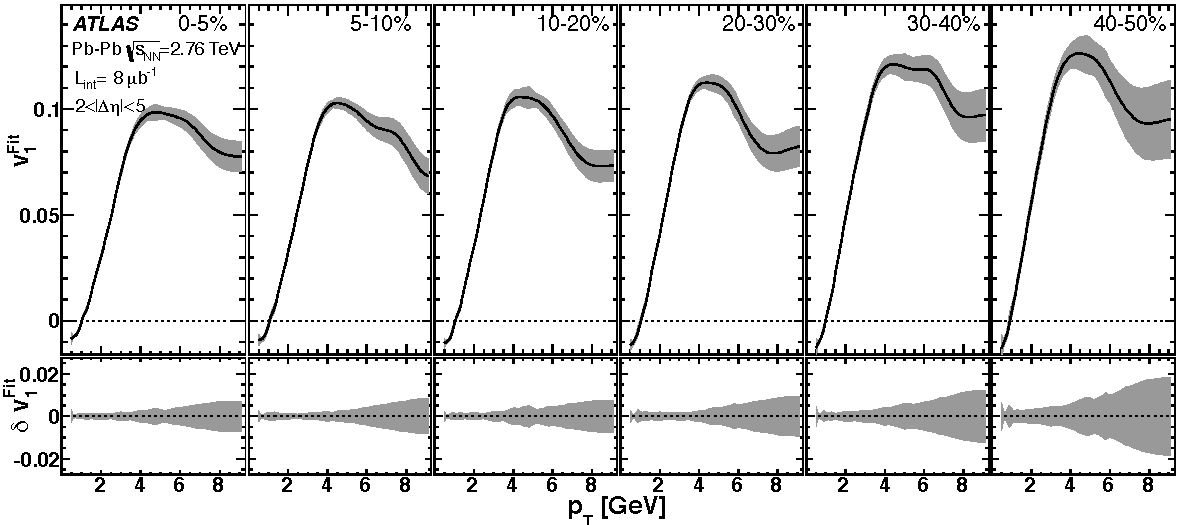
\includegraphics[width=0.98\textwidth]{flowcorrelations_figs/atlas_vn_fig_21.pdf}
\caption[]{
(top) ATLAS data showing the amplitude of $v_{1,1}$ the dipole modulation in the 2-particle correlation function, as a function of $p^b_T$ for ranges in $p^a_T$.  The fit used to extract the functional form of $v_1(\pT)$ is shown.
(bottom) The extracted functional form of $v_1(\pT)$, from the fits shown above, as a function of centrality.
}
\label{fig:pas:fc:v1}
\end{center}
\end{figure}

\begin{figure}[!htb]
\begin{center}
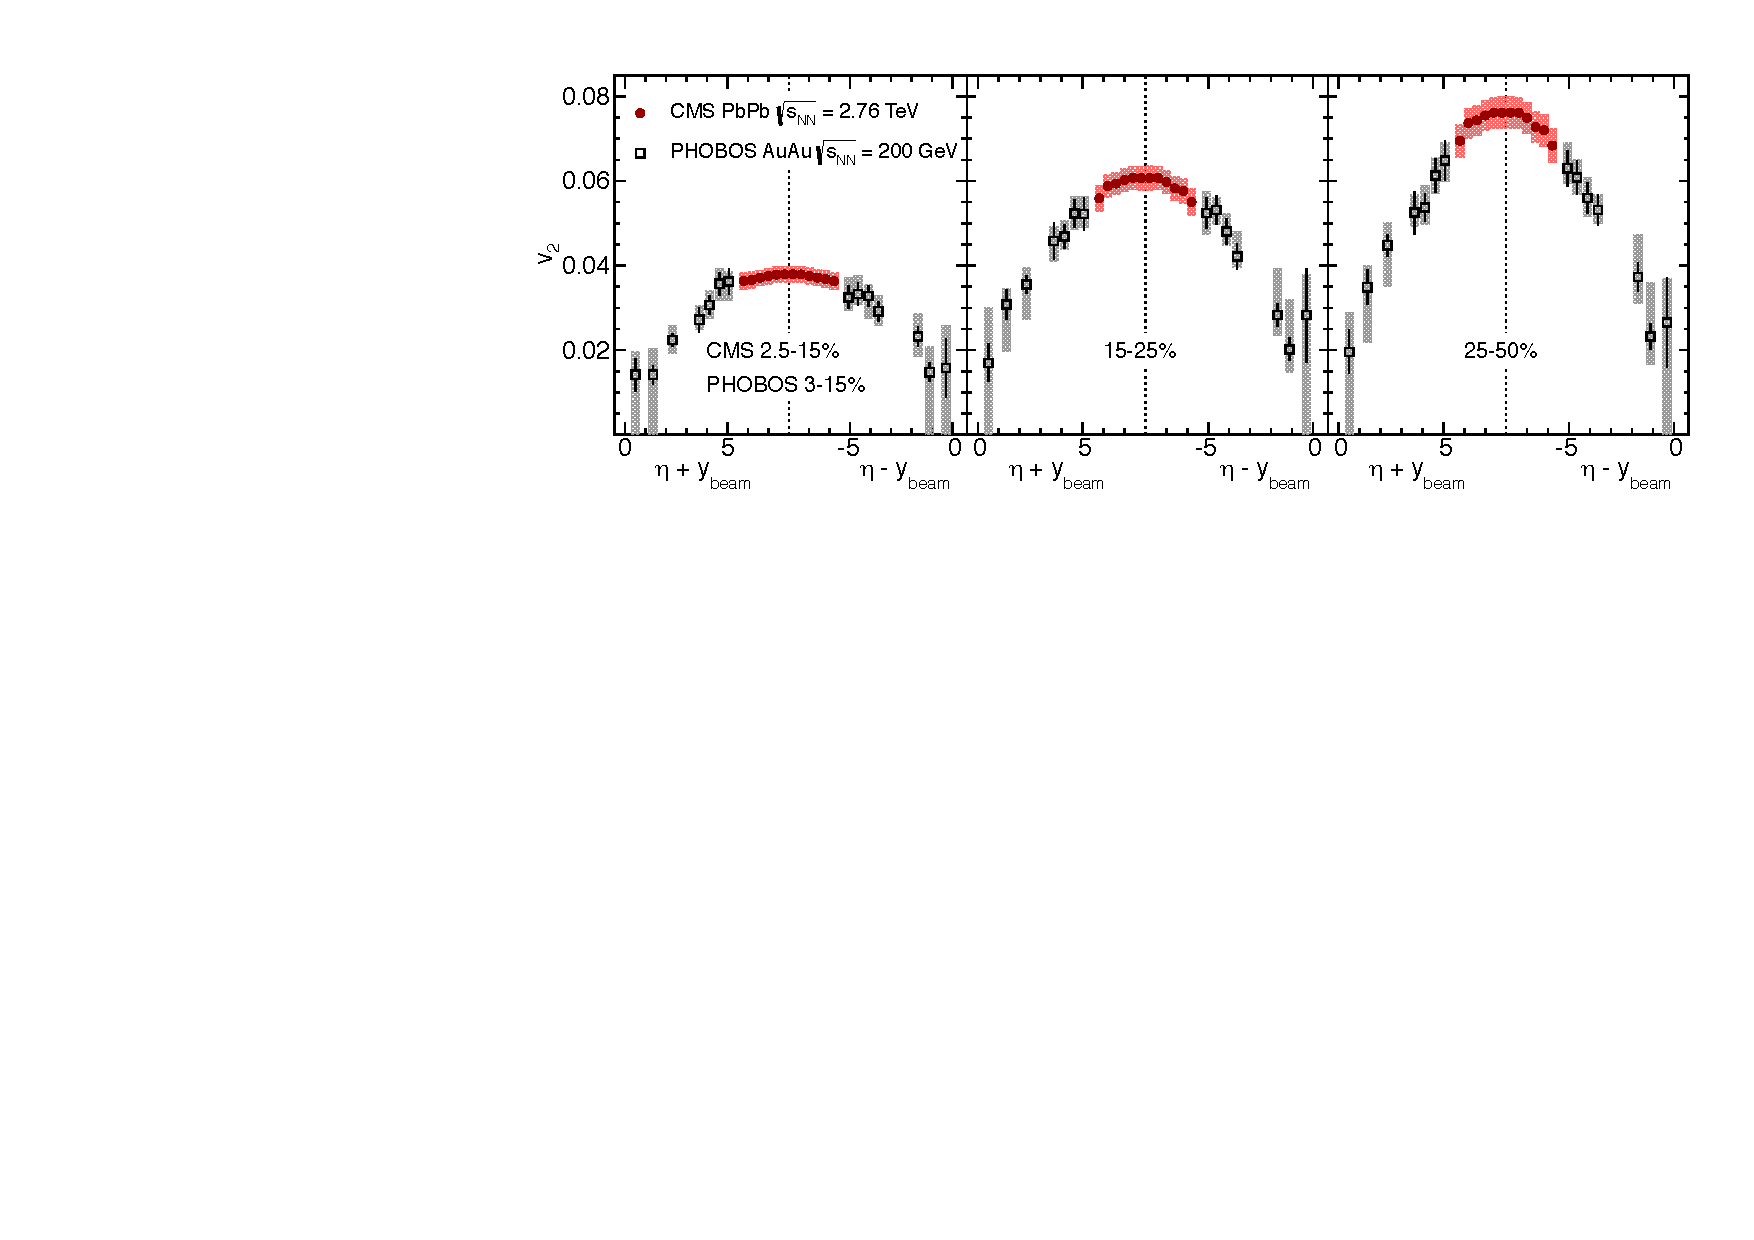
\includegraphics[width=0.98\textwidth]{flowcorrelations_figs/v2_etashifted_3cen_PHOBOS.pdf}
\caption[]{
CMS data showing $\vtwo$ for unidentified hadrons as a function of $\eta - y_{\mathrm{beam}}$, averaged over $0 <\pT < 3$ GeV (using an extrapolation procedure to cover $\pT <300$ Mev).
Results are compared to data from $\sqrt{s_{NN}}=200$ GeV
at large $\eta$ from the PHOBOS experiment at RHIC.
}
\label{fig:pas:fc:limfrag}
\end{center}
\end{figure}

\begin{figure}[!htb]
\begin{center}
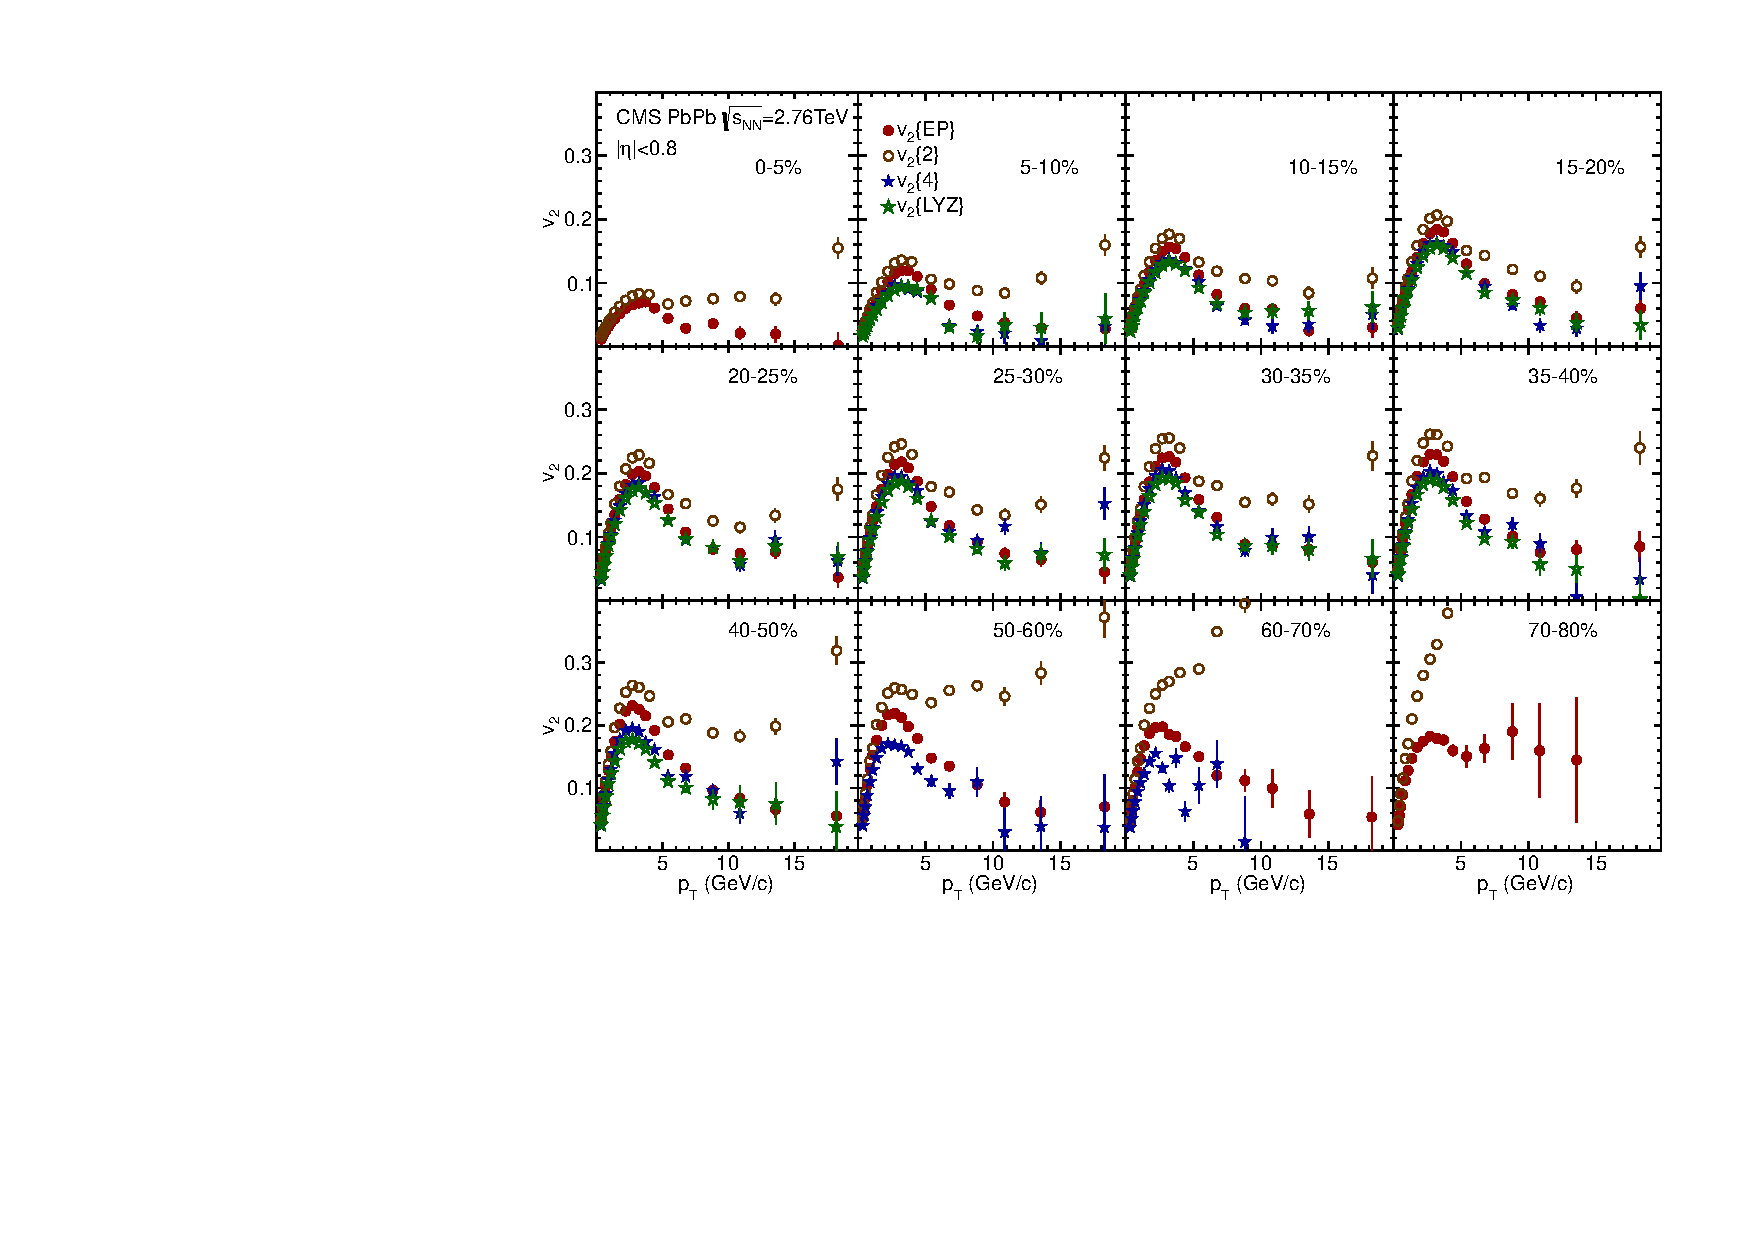
\includegraphics[width=0.98\textwidth]{flowcorrelations_figs/v2_pt_12cen_4methods.pdf}
\caption[]{
CMS data showing $\vtwo(\pT)$ in centrality intervals, using four different methods of extracting
$\vtwo$: event plane (EP), 2-particle cumulants, 4-particle cumulants, and Lee-Yang Zeros.
}
\label{fig:pas:fc:methods}
\end{center}
\end{figure}




\section{Electroweak probes}
% change

\section{Jet quenching}
\label{jets_intro}

The vastly increased production cross sections for very high \pT\ hard-scattered jets at the LHC
compared to RHIC, combined with the moderate growth of soft particle production forming the ``underlying
event'', opened a new era in studies of jet quenching. The improved signal to background allowed the
use of standard reconstruction techniques, calibration methods, background subtraction methods and
jet observables developed and well characterized for studies of \pp\ collisions.
Typically jets in LHC heavy-ion collisions are reconstructed using
the infrared-safe anti-$k_t$ jet clustering algorithm~\cite{Cacciari:2008gp} with the
radius parameter $R$ varying from $0.2 < R  < 0.5$. Differences between the three
experiments exist in the approach to ``background subtraction'', i.e., the correction
of the reconstructed jet energie for contributions from the \PbPb\ underlying event. 
ATLAS and CMS employ iterative correction methods where jet candidates found in
the first iteration are removed from the background estimate~\cite{Kodolova:2007hd,Grau:2008ed},
while ALICE uses the median area-density method provided by the {\sc{fastjet}} package~\cite{Cacciari:2011ma}.
Importantly, the ALICE and ATLAS corrections are applied on the reconstructed jet energies,
while the CMS correction is applied to the input objects of the jet clustering algorithm.
Differences also exist in the effective energy or momentum cutoff of the jet constituents,
which can have a significant influence on the noise introduced by the underlying event~\cite{Abelev:2012ej}.

Early measurements of hadron production at RHIC
clearly showed a large suppression (up to a factor of five to six) in the production rates of
high \pT\ particles in heavy-ion collisions compared to a properly scaled \pp\ reference distribution
\cite{Adcox:2001jp,Adler:2002xw}. Similarly, the ``jet quenching'' phenomenon was observed
in the suppression of back-to-back hadron production
in central heavy ion collisions~\cite{Adcox:2001jp,Adler:2002xw}. Yet nearly a decade after the first observation, a detailed
understanding of the physics of parton energy loss in the hot and dense medium remained
elusive. A review of the theoretical state-of-the art before LHC startup can be
found in ~\cite{Wiedemann:2009sh}.

Compared to hadron-based observables such as those employed at RHIC, measurements of reconstructed
jet, dijet and photon-jet final states promise much greater control over the type and kinematics
of the initial scattering process and access to information about the energy flow in the evolution
of the collision process not otherwise accessible.

\subsection{Dijet correlations}

The first jet-based observables discussed here are derived from dijet correlations. Within hours
after the first heavy-ion collisions at LHC were recorded, it became obvious that there was
a large abundance of events were a high \pT\ reconstructed jet (e.g. $\pT \approx 100$\GeVc) was
not accompanied by a back-to-back high \pT\ partner jet.

In the first study of jets in \PbPb\ collisions at LHC, ATLAS used azimuthal correlations and the
momentum asymmetry between the leading and subleading jets to characterize the modification
of their properties relative to \pp\ collisions \cite{Aad:2010bu}.
The jet pairs were selected to have relative azimuthal angle $\dphi =|\varphi_1-\varphi_2| > \pi/2$
and their momentum asymmetry was determined as
\begin{equation}
A_J = \frac{E_{T1}-E_{T2}}{E_{T1}+E_{T2}}.
\end{equation}
The leading jet was required to have a transverse energy in the calorimeter of $E_{T1} > 100$~GeV,
and the subleading jet was selected to have $E_{T2} > 25$~GeV, after correction for
the calorimeter energy response.

In Fig.~\ref{fig:GR:final_4x2} the dijet asymmetry and $\dphi$ distributions 
for \PbPb\ data (solid markers)
are shown in four bins of collision centrality. They are compared with PYTHIA MC calculations, including a
background simulation using the HIJING event generator. Also shown are data from 7\TeV\
\pp\ collisions (open circles).
\begin{figure}[!thb]
\begin{center}
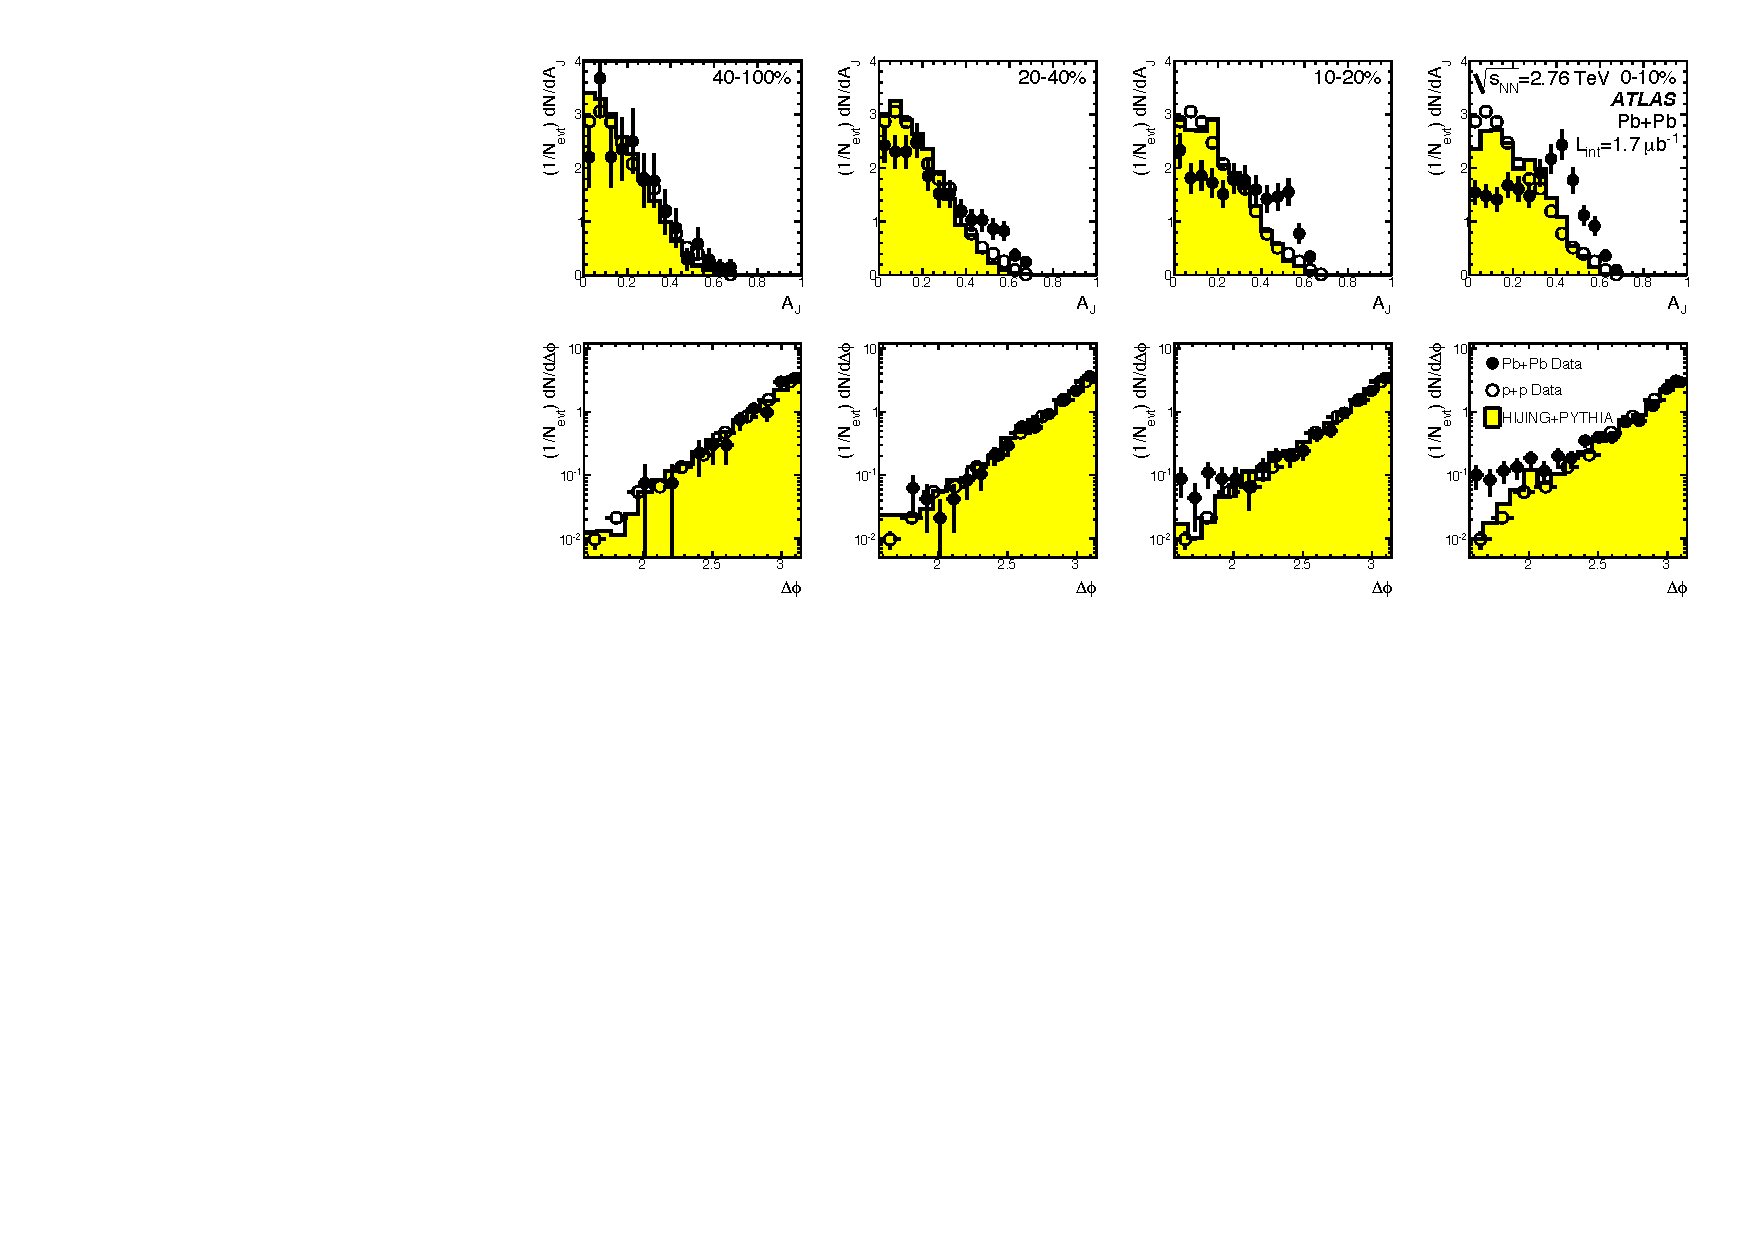
\includegraphics[width=0.8\textwidth]{jetfigures/final_4x2_23_newpp.pdf}
\caption{
(top) Dijet asymmetry distributions for data (points) and {\sc{hijing+pythia}} 
simulations (solid yellow histograms), as a function of collision centrality.  
Proton-proton data from $\sqrt{s}=7$\TeV\ is shown as open circles.
(bottom) Distribution of $\dphi$ between the two jets, 
for data and {\sc{hijing+pythia}}, shown in four bins of centrality.
Reproduced from~\cite{Aad:2010bu}.}
\label{fig:GR:final_4x2}
\end{center}
\end{figure}

A clear centrality evolution of the dijet asymmetry distribution can be seen, while the azimuthal
dijet correlations remain largely unchanged. For peripheral events, the \PbPb\ dijet asymmetry
is comparable to that seen in PYTHIA and \pp\ collisions. For central events however,
the $A_J$ distribution widens significantly, showing a large increase in unbalanced
dijet events. 
A similar measured by CMS, using the full 2010 \PbPb\ data set, confirmed these 
observations~\cite{Chatrchyan:2011sx}.
The observed trend can be naturally understood in models of parton energy
loss in the hot and dense medium, where the back-to-back partons will typically traverse
different path lengths, and therefore suffer different amounts of energy loss. 

The initial ATLAS and CMS dijet asymmetry analyses were extended using a 
large dataset of \PbPb\ collisions
collected in 2011 by the CMS collaboration at $\rootsNN=2.76$\TeV~\cite{CMS_dijet}. For this analysis, the events were 
reconstructed using the  CMS ``particle-flow" algorithm~\cite{CMS-PAS-PFT-10-002,MattPFlow}, 
which attempts to identify all stable particles in an
event (electrons, muons, photons, charged and neutral hadrons)
by combining information from all sub-detector systems.
Jets were then reconstructed, after background subtraction, using the anti-$k_T$ algorithm 
with radius parameter R = 0.3~\cite{Cacciari:2008gp}.

Figure~\ref{fig:GR:CMS_dijet_pt} presents the dijet asymmetry in bins of leading jet
\pT, for 0--20\% central events, allowing a study the momentum dependence of the amount of energy loss.
The distributions show the \ptrat\ ratio, instead of $A_j$,  as a more intuitive
way of quantifying the dijet momentum asymmetry.

\begin{figure}[!th]
\begin{center}
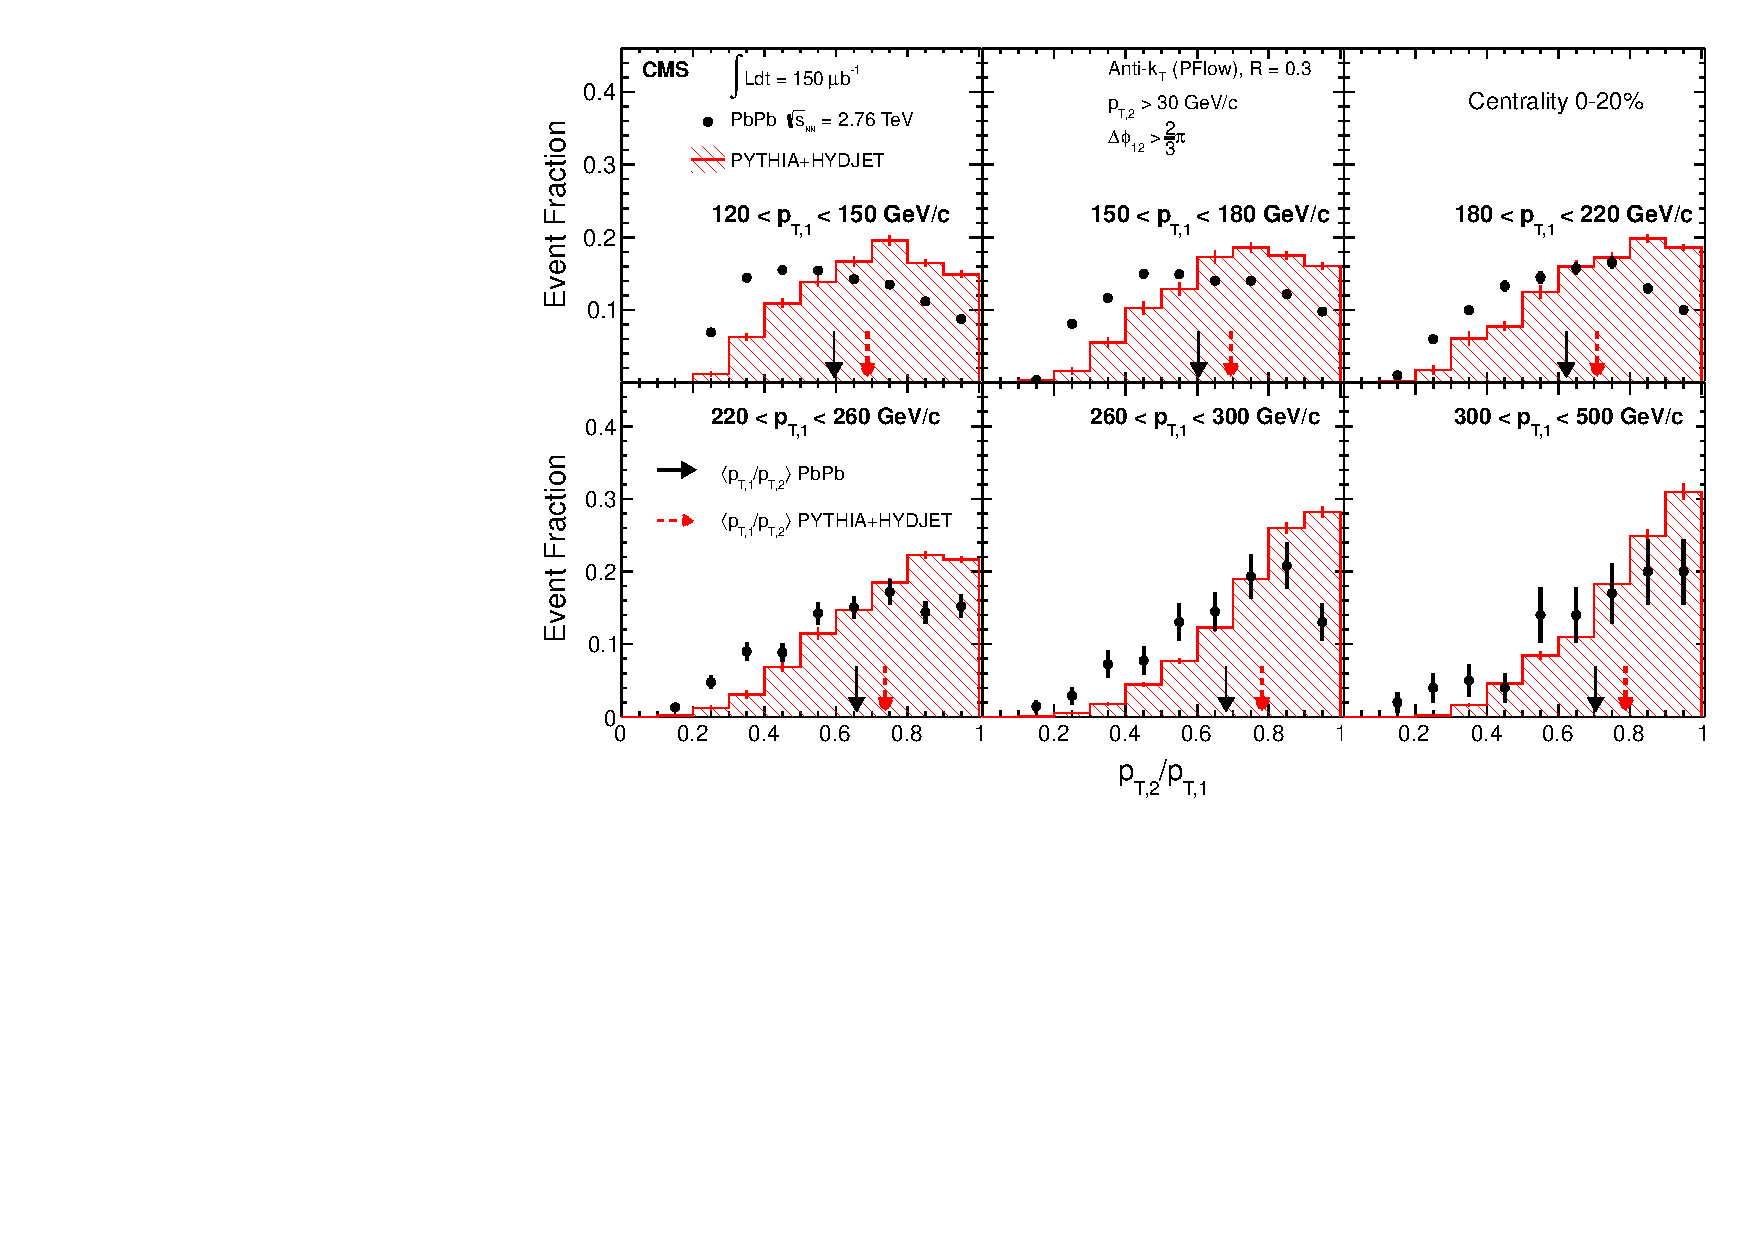
\includegraphics[width=0.6\textwidth]{jetfigures/dijet_imbalance5_0to20_pt_20120103_subt.pdf}
\caption{Dijet asymmetry ratio, $A_{J}$, in bins of leading jet transverse momentum from
120 $ < \ptlead < 150$~GeV/c to $\ptlead > 300$~GeV/c for
  subleading jets of $\ptsub> 30$~GeV/c
and $\dphi>2\pi/3$ between leading and subleading jets.
Results for 0--20\% central \PbPb\ events are shown as points, while the histogram
shows the results for
PYTHIA dijets embedded into HYDJET \PbPb\ simulated events. The error bars represent the statistical uncertainties.
Reproduced from~\cite{CMS_dijet}.}
\label{fig:GR:CMS_dijet_pt}
\end{center}
\end{figure}
One observes a strong evolution in the shape of the distribution across the
various \pT\ bins. However, a significant difference between \PbPb\ data and
\PYTHYD\ simulations persists even for the highest \pT\ bin.
The jet momentum dependence of the energy loss can then be examined by measuring the
average dijet asymmetry as a function of leading jet momentum. This was studied by CMS,
using $\langle \ptsub/\ptlead \rangle$. Figure~\ref{fig:GR:CMS_pt_ratio}
shows the \pT\ dependence of this ratio for three
bins of collision centrality, with \PYTHYD\ simulations shown
as squares and \PbPb\ data shown as points.

\begin{figure}[!th]
\begin{center}
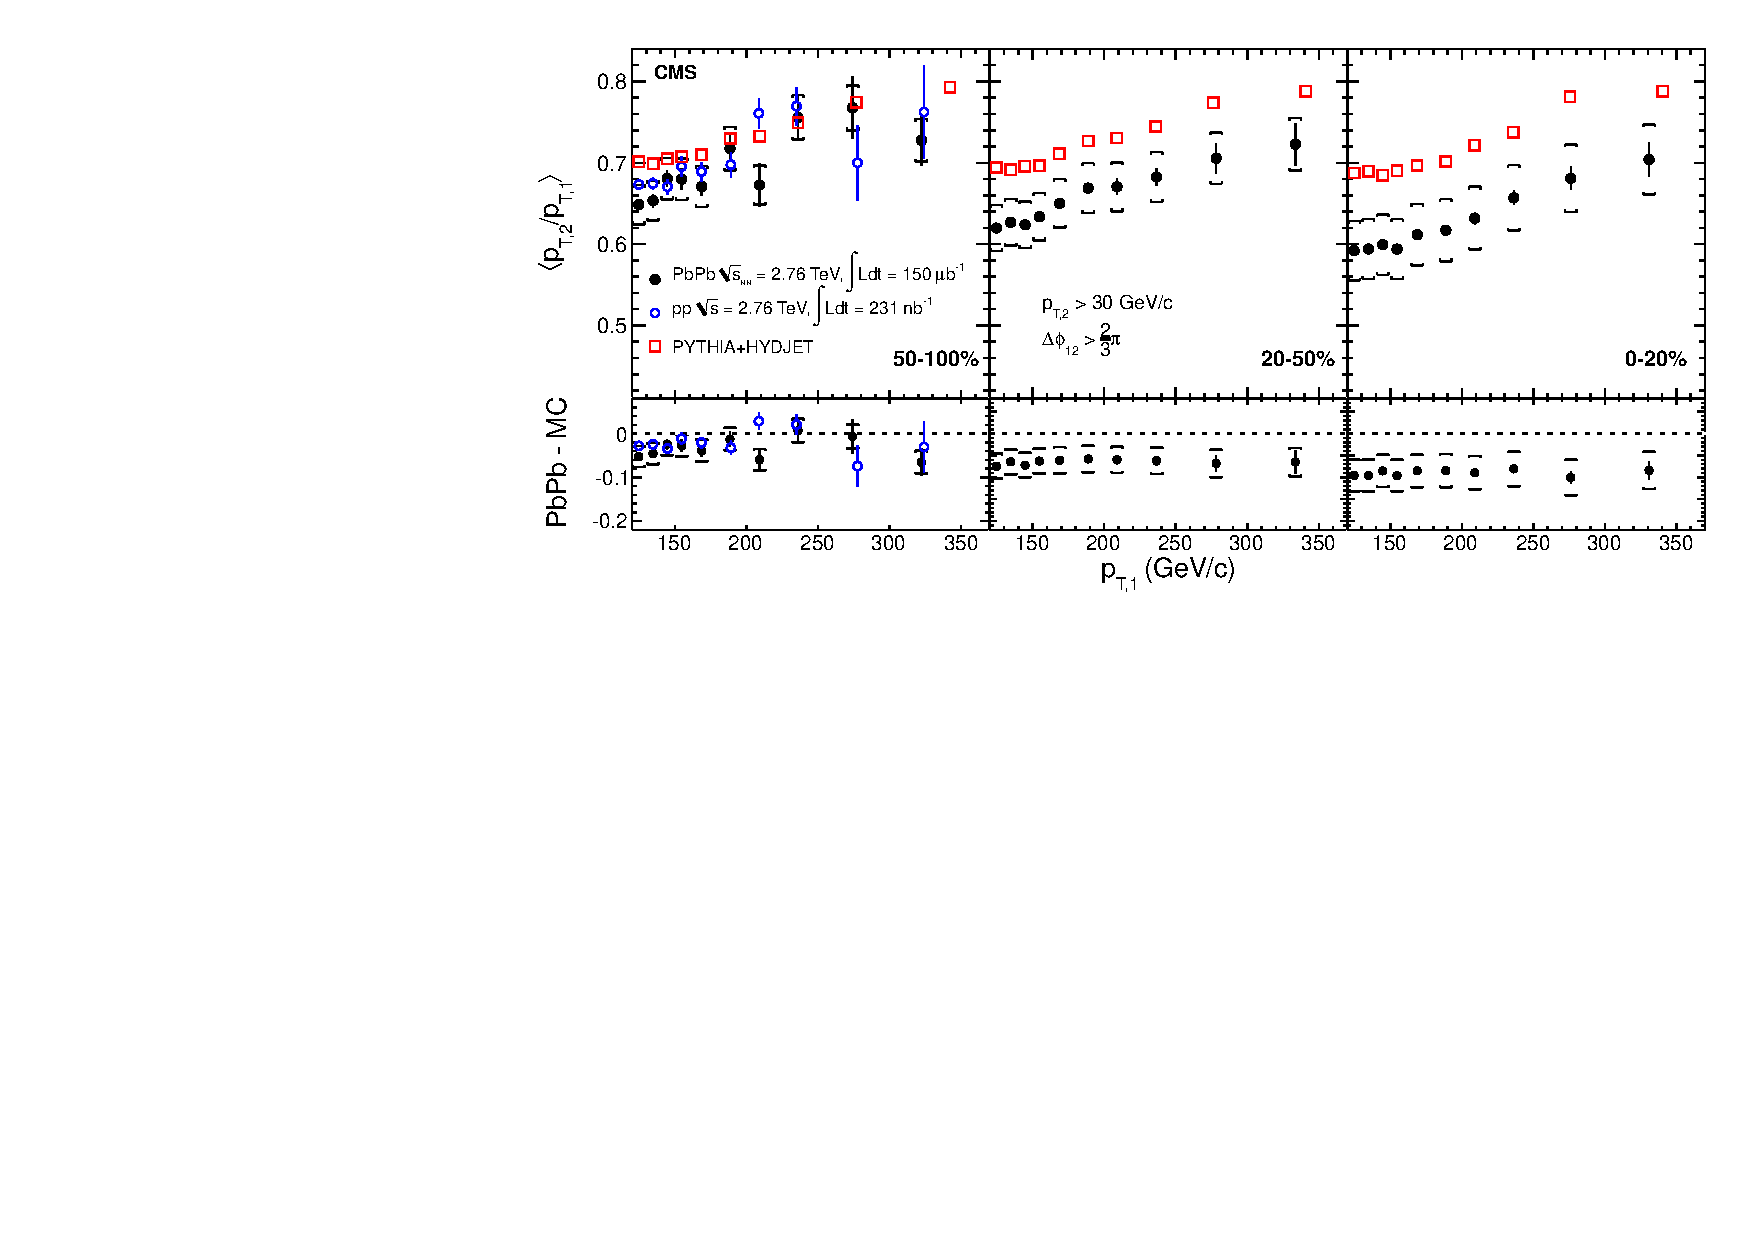
\includegraphics[width=0.6\textwidth]{jetfigures/deltaPtOverPt5_lead120_sub30_diff_20120103.pdf}
\caption{(Top): Dijet momentum ratio $\langle \ptsub/\ptlead \rangle$ as a function of
leading jet \pT\ in three bins of collision centrality.
\PbPb\ data are shown as points, with brackets indicating systematic uncertainties.  
\PYTHYD\ calculations are shown as squares. In the peripheral bin,
\pp\ data are displayed as open circles.
(Bottom): Difference of $\langle \ptsub/\ptlead \rangle$ between the \PbPb\ results and \PYTHYD\ reference.
Reproduced from~\cite{CMS_dijet}.}
\label{fig:GR:CMS_pt_ratio}
\end{center}
\end{figure}

For all data and simulations, a rising trend of $\langle \ptsub/\ptlead \rangle$ as a function
of leading jet momentum is seen. This is a result of the improving jet energy resolution
with increasing jet \pT\ and the evolution in jet kinematics, which is described by the PYTHIA
calculations. Importantly, the data show a significantly larger jet asymmetry in central events
than in the simulations and in peripheral and \pp\ data. This effect persists to the
highest \pT\ measured, showing that even the highest \pT\ jets in \PbPb\ collisions ($\pT > 350$\GeVc)
suffer energy loss as they traverse the medium. A detailed understanding of the energy loss
\pT\ dependence (e.g.\ fractional vs constant energy loss) will require a full jet MC calculation
taking the detector response as a function of \pT\ into account.

\subsection{Suppression of jet yields}

A complementary approach to the study of parton energy loss using dijet asymmetry measurements
is offered by studies of the nuclear modification factor \Raa\ of jet yields relative
to a \pp\ reference or the centrality evolution of \Rcp\ relative to peripheral events.

Measurements of the inclusive jet production rates were performed by ATLAS~\cite{Aad:2012is} and 
ALICE~\cite{Abelev:2013kqa}.
As a result of the path length dependence of parton energy loss in the medium, 
a reduction in the observed jet yield at a given \pT\ is expected for more 
central \PbPb\ collisions, compared to an \Ncoll\ scaled \pp\ or peripheral reference.

\begin{figure}[!th]
\begin{center}
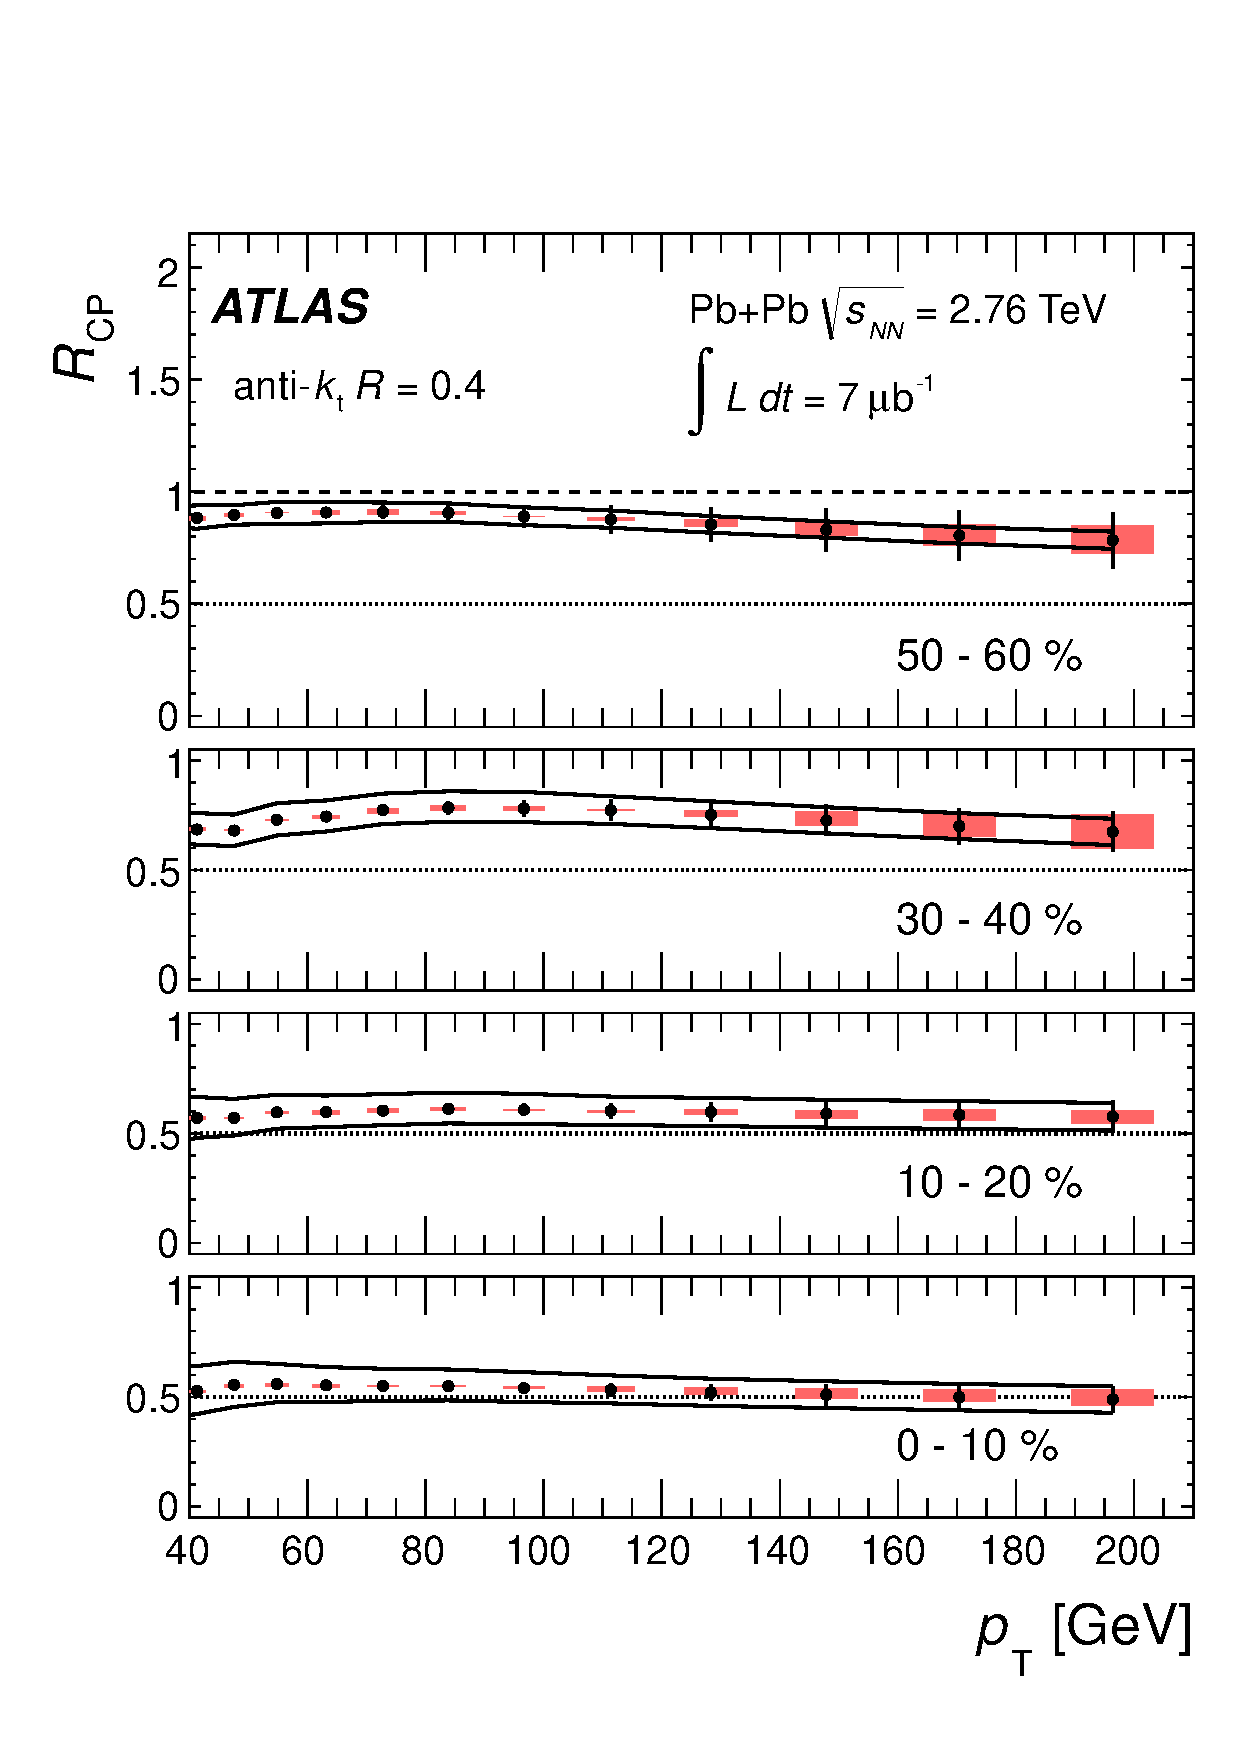
\includegraphics[width=0.49\textwidth]{jetfigures/ATLAS_jetRCP_04.pdf}
\caption{
\pT\ dependence of jet \Rcp\ for  $R=0.4$ jets,
in four bins of collision centrality. Error bars indicate
statistical errors while shaded boxes indicate
partially correlated systematic uncertainties. 
The solid lines show fully correlated uncertainties. Reproduced from~\cite{Aad:2012is}.}
\label{fig:GR:rcprfour}
\end{center}
\end{figure}
The resulting \Rcp\ values are shown in Figure~\ref{fig:GR:rcprfour}
for  \RFour\ jets as a function of jet \pT\ in four bins
of collision centrality.
Uncertainties are shown as statistical uncertainties, partially correlated systematic
uncertainties, and fully correlated uncertainties.

For all centralities only a weak dependence of \Rcp\ on jet \pT\ is observed.
In contrast, a strong suppression of the jet yield is evident in
central collisions, with \Rcp\ only reaching a value of about 0.5.
This is reminiscent of the value of charged hadron \Raa\ observed
by CMS at very high \pT\, which also reaches a value of about 0.5.
The centrality evolution of \Rcp\ is consistent with expectations
based on the increasing in-medium pathlength traversed by the partons.

Further insight into the pathlenth dependence of parton energy
loss may be gained by studying the dependence of the jet yield
on the jets azimuthal angle relative to the event plane
in peripheral \PbPb\ collisions. This allows the selection of jets
traversing different length of the medium at the same medium
conditions, whereas the centrality dependence of \Rcp\ reflects
both the changing pathlength and potential changes in the medium
density with centrality.

Related measurements have been performed using the azimuthal dependence
of charged hadron yields at intermediate \pT\
\cite{Adams:2004wz,Adler:2006bw,Adare:2010sp, ATLAS:2011ah, Abelev:2012di}.
and very high \pT \cite{Chatrchyan:2012xq}. For mid-peripheral events,
a finite \vtwo\ for charged hadrons was observed for \pT\ in excess of 40\GeVc.
Compared to these results, jet based measurements offer the advantage
of a more direct relationship between \pT\ and direction of the observed
jet and the initial parton.

\begin{figure}[!th]
\begin{center}
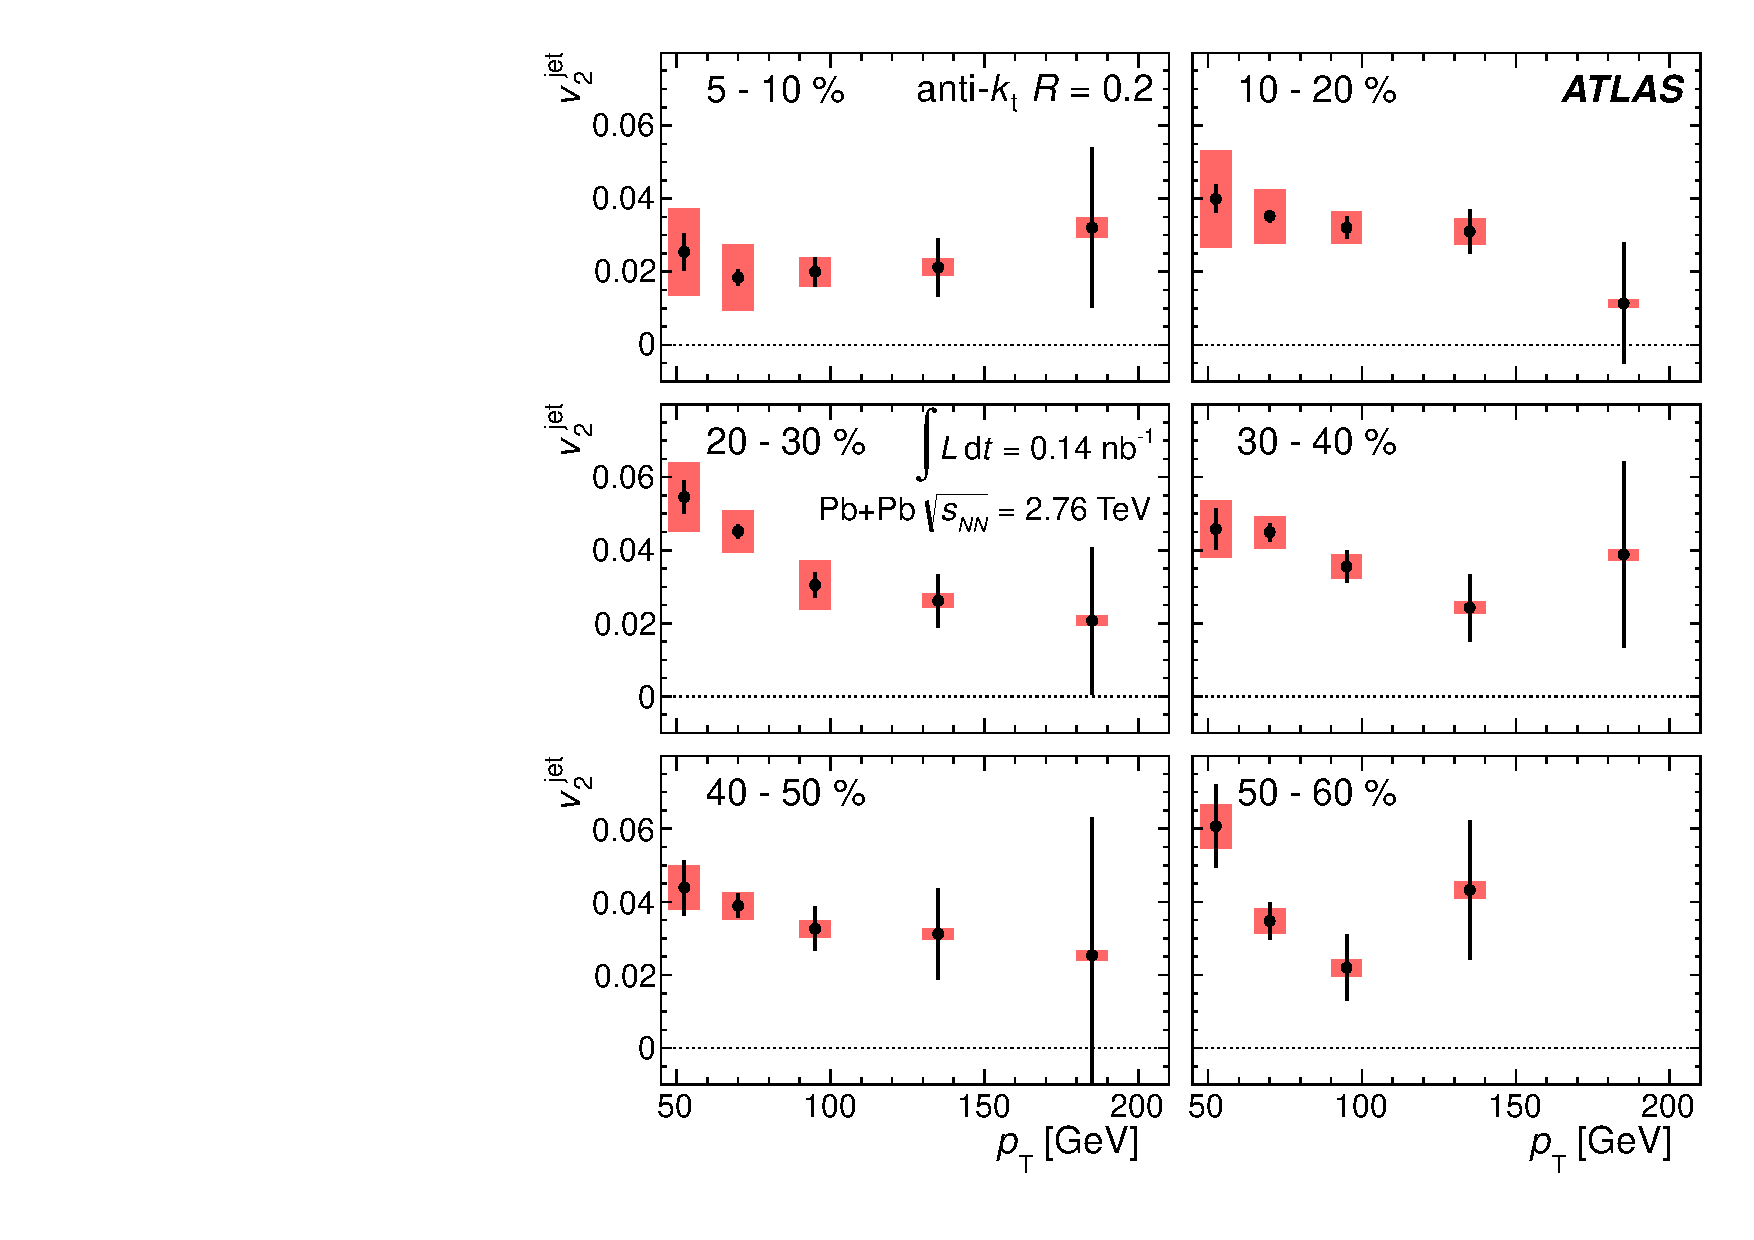
\includegraphics[width=0.49\textwidth]{jetfigures/ATLAS_jetv2.pdf}
\caption{\vtjet\ as a function of jet \pT\ in six bins of 
collision centrality.
Error bars indicate statistical uncertainties and 
systematic uncertainties are shown as shaded boxes. Reproduced from~\cite{Aad:2013sla}}
\label{fig:GR:ATLAS_jet_v2}
\end{center}
\end{figure}

The result of the ATLAS \vtwo\ measurement for jets reconstructed with the anti-$k_T$
algorithm in 2.76\TeV\ \PbPb\ collisions is shown in Fig.~\ref{fig:GR:ATLAS_jet_v2}
as a function of jet \pT\ in bins of collision centrality~\cite{Aad:2013sla}. A finite
value of \vtwo\ is observed for all centrality and \pT, reaching up to 0.05 for
mid-central collisions and low jet \pT. The results are in good agreement
with those for high \pT\ charged hadrons covering a comparable range
of initial parton \pT~\cite{Chatrchyan:2012xq}.

\subsection{Modification of jet structure}

In addition to the \pT\ and centrality dependence of the suppression, its dependence on the 
jet clustering radius parameter or cone-size is also of great interest, as different energy loss 
mechanisms may lead to different amounts of energy transport out of the jet cone
\cite{Vitev:2008rz, Vitev:2009rd,He:2011pd}. This should manifest as a cone-size
dependence of the observed jet suppression.
\begin{figure}[!th]
\begin{center}
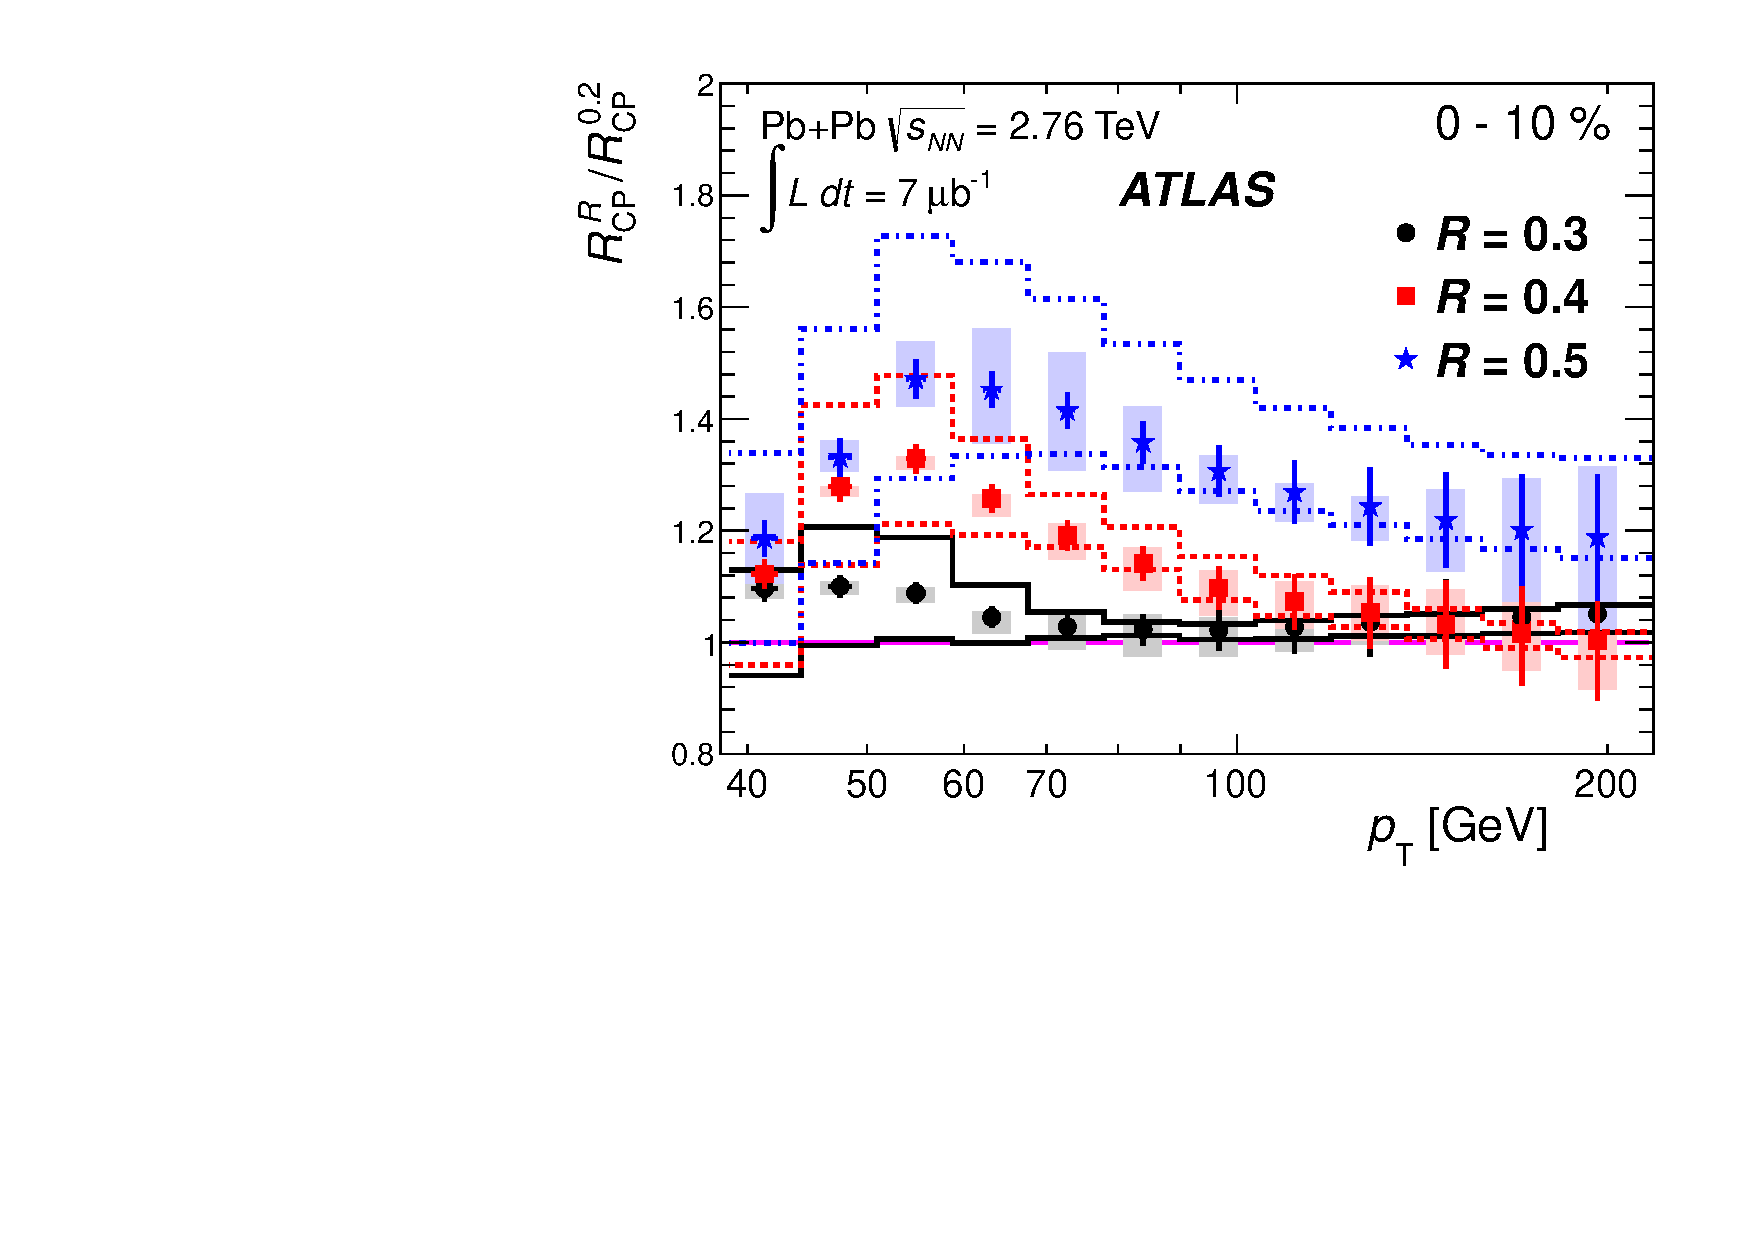
\includegraphics[width=0.49\textwidth]{jetfigures/ATLAS_jetRCP_size.pdf}
\caption{
Ratios of \Rcp\ values between $R = 0.3, 0.4$ and 0.5 jets and $R =
0.2$ jets as a function of \pT\ in the 0--10\% centrality bin. The
error bars show statistical uncertainties. The shaded boxes
indicate partially correlated systematic errors. The lines indicate
systematic errors that are fully correlated between different \pT\ bins.
Reproduced from~\cite{Aad:2012is}.
}
\label{fig:GR:ATLAS_jetRCP_size}
\end{center}
\end{figure}

Such a dependence can be seen in Fig.\ref{fig:GR:ATLAS_jetRCP_size}, which shows
shows the ratio of \Rcp\ values for $R = 0.3, 0.4$ and 0.5 jets compared
to an $R = 0.2$ jets baseline, as a function of \pT\ for central events,
measured by ATLAS~\cite{Aad:2012is}.

The cancellation of various systematic uncertainties allows the observation of a
a significant jet radius dependence of \Rcp, in particular for
lower jet \pT. A detailed comparison needs to consider the \pT\ associated with
using different radius parameters to reconstruct the same jets.

Further insight into modifications of the momentum and angular structure
of jets in heavy-ion collisions can be gained by measurements of
observables used for jet studies in elementary interactions, such as
fragmentation functions and jet shapes.
Fragmentation functions describe the probability for a parton to fragment into
hadrons carrying certain fractions of the parton energy.
In vacuum, the parton radiation and splitting processes lead to a
well-understood characteristic shape of the fragmentation function \cite{Dokshitzer:1991wu}.

\begin{figure}[!ht]
\begin{center}
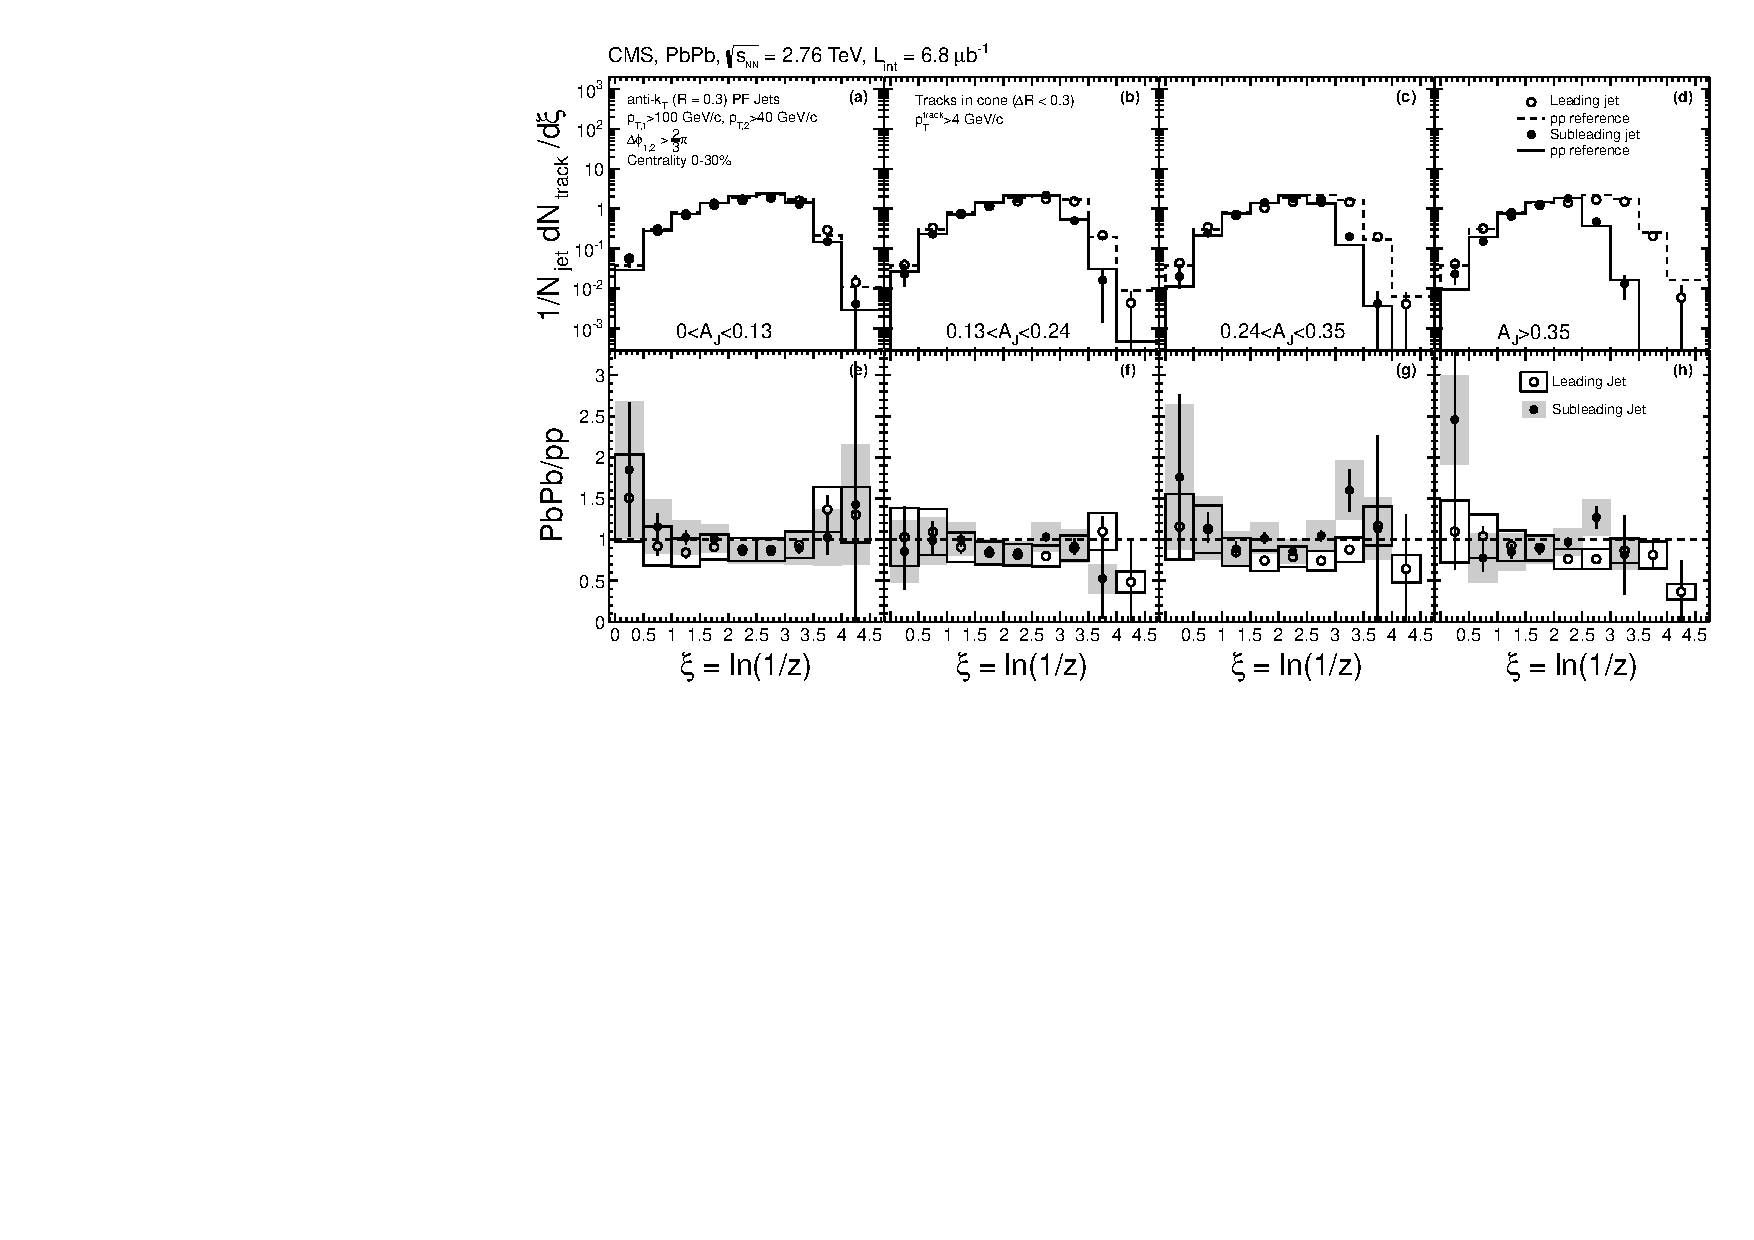
\includegraphics[width=0.8\textwidth]{jetfigures/xsi_div_both_effv9_l100s40_0to12_dphi20eta20dr3pt4id1_cwt_ppDiv_gray.pdf}
\caption{Top row: Fragmentation functions for the leading (open circles) and subleading (solid points) 
jets in four regions of $\AJ$ in central \PbPb\ collisions compared to the \pp\ reference.
Bottom row: Ratio of each fragmentation function to its \pp-based reference.
Error bars shown are statistical. The systematic uncertainty is
represented by open boxes (leading jet) or gray boxes (subleading jet).
Reproduced from~\cite{Chatrchyan:2012gw}.
}

\label{fig:GR:CMS_jetFF}
\end{center}
\end{figure}
Figure~\ref{fig:GR:CMS_jetFF} shows the fragmentation functions for
for leading and subleading jets for 0-30\% central collisions, obtained
by CMS~\cite{Chatrchyan:2012gw}. Data for \PbPb\ are shown in 
bins of dijet asymmetry $A_J$, and compared to a \pp\ based reference.
The lower row of plots shows the ratio of the ratios between the \PbPb\
and \pp-based fragmentation functions. It is important to note, and has 
led to occasional confusion, that these fragmentation functions are 
measured relative to the \em observed\em jet momentum, not with respect
to the initial parton momentum, which can not be directly observed
for dijet events in hadronic collisions.

Within the uncertainties of this first measurement, no significant modification of
the fragmentation functions in \PbPb\ collisions is observed. This is true even for
dijets with large asymmetry, i.e.\ where the subleading jet has suffered significant
energy loss. It is important to note however that only hadron fragments with $\pT > 4$\GeVc
have been considered in this measurement.

Complementary information about the angular structure of the jets and its modification
by the in-medium shower evolution can be obtained by measuring jet shapes, i.e.\ the
jet transverse momentum profile as a function of radial distance to the jet axis
\cite{MehtarTani:2010ma,Idilbi:2008vm,CasalderreySolana:2011rz,CasalderreySolana:2011rq,Neufeld:2011yh,Blaizot:2012fh,Fickinger:2013xwa}.
The differential jet shape, $\rho(r)$, is defined as
\begin{equation}
\rho(r) = \frac{1}{\delta r} \frac{1}{N_{\mbox{jet}}} \sum_{\mbox{jets}}
\frac{\sum\limits_{{r - \delta r/2}}^{{r + \delta r/2}}{\pT^{\mbox{track}}}}{\pT^{\mbox{jet}}}
\label{eq:rho(r)}
\end{equation}
Here $r$ is the radial distance from the jet axis
and the transverse momenta of the reconstructed track and jet are
$\pT^{\mbox{jet}}$ and $\pT^{\mbox{track}}$, respectively.

In the CMS measurement of jet shapes\cite{Chatrchyan:2013kwa}, the jet cone is divided into six concentric rings
with radial width $\delta r = 0.05$. The transverse momentum profile is determined using
the \pT\ sum for charged particles with $\pT > 1\GeVc$ in each ring, compared to
the fraction of the total jet \pT\ carried by these particles. As for the fragmentation
functions, the \PbPb\ jet shapes are compared to a \pp\ based reference.

\begin{figure}[!ht]
\begin{center}
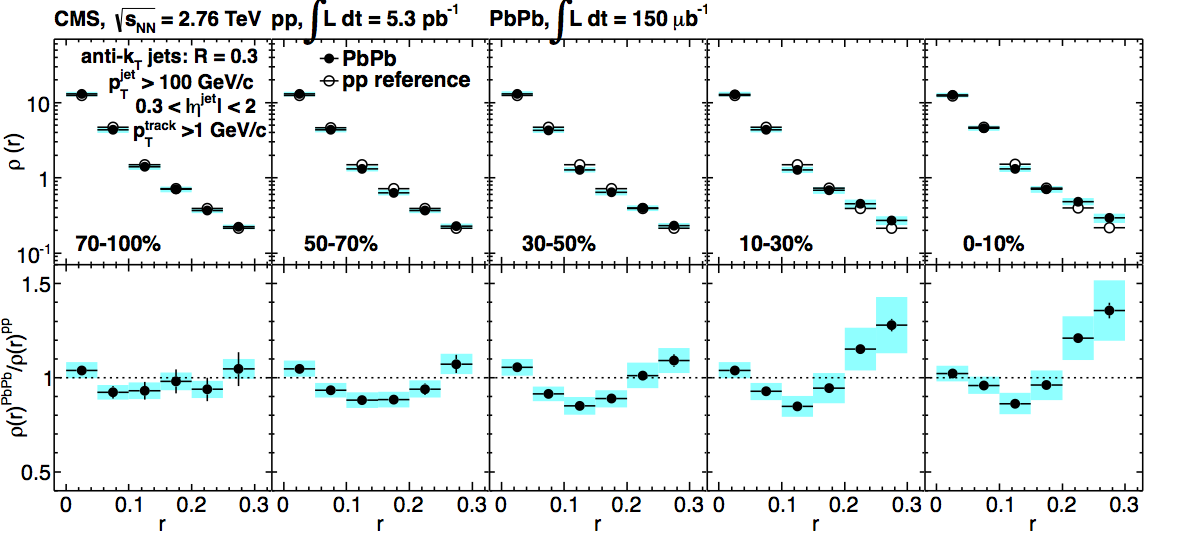
\includegraphics[width=0.98\textwidth]{jetfigures/JetShapes_GR.png}
\caption{\label{fig:JSRatio}
(Top): Differential jet shapes in \PbPb\ collisions (filled circles)
as a function of distance from the jet axis for inclusive jets with $\pT^{\mbox{jet}} >100\GeVc$
in five bins of centrality.  The \pp-based reference is shown with open symbols.
The shaded regions represent the \PbPb\ systematic uncertainties.
Statistical uncertainties are smaller than the marker size.
(Bottom): Jet shape ratios $\rho(r)^{\PbPb}/\rho(r)^{\pp}$.
Error bars show the statistical uncertainties and shaded boxes indicate the systematic uncertainties. 
Reproduced from~\cite{Chatrchyan:2013kwa}}
\label{fig:GR:CMS_jetshapes}
\end{center}
\end{figure}

The top row of Fig.~\ref{fig:GR:CMS_jetshapes} shows the differential jet shapes measured in \PbPb\
collisions and the \pp\ based reference, while the bottom row shows the ratio of the \PbPb\ and \pp\
distributions. The results are presented in five bins of collision centrality, from
most peripheral 70--100\% (left) to most central 0--10\% (right). For
both systems, only a small amount of the total jet energy
is carried by particles more than  $r> 0.2$ away from the jet axis. However, for central
\PbPb\ collisions a large enhancement of the energy fraction at the largest distance
to the jet axis ($r = $0.25-0.3) can be seen.
This is qualitatively consistent with the \Rcp\ ratios for different jet radii seen by ATLAS,
where also an additional part of the jet energy is captured when moving beyond $R = 0.2$.
This observation is in line with the trends predicted in
\cite{Vitev:2008rz,Renk:2009hv}, although these calculations were
done for a different energy and and at parton level rather than hadron level.

\subsection{Energy flow in dijet events}

The jet measurements discussed so far clearly demonstrate that partons traversing the hot and dense
medium suffer significant path-length dependent energy loss. A fraction of the ``lost'' energy
can be recovered at radii of $r=$0.2-0.5 from the jet axis, although even for the largest radius
parameters used at LHC, a large suppression of inclusive jets and large dijet asymmetries are
observed.

This naturally begs the question of the detailed energy flow in the events containing asymmetric
dijets events, i.e.\ what is the angular and momentum distribution of the particles carrying
the complementary momentum balance to the asymmetric dijet system? A priori the energy balance
could possibly be found at low (thermal) momenta and very large radial distance to the jet axis.
Therefore traditional jet-track correlation techniques relying on background subtraction are ill suited
to answer this question, as even the largest dijet energy differences of several 10's of \GeV\
are much smaller than fluctuations in the transverse energy carried by the underlying event.

Information about the overall momentum balance in the dijet events can be obtained by exploiting
conservation of transverse momentum. CMS studied the transverse momentum balance in these events
using the projection of missing \pT\ of reconstructed charged tracks onto the leading 
jet axis~\cite{Chatrchyan:2011sx}. 
Event-by-event, this was calculated as 
\begin{equation}
\displaystyle{\not} p_{\mathrm{T}}^{\parallel} =
\sum_{\rm i}{ -p_{\mathrm{T}}^{\rm i}\cos{(\varphi_{\rm i}-\varphi_{\rm Leading\ Jet})}},
\end{equation}
summing all tracks with $\pT > 0.5$~\GeVc\ and $|\eta| < 2.4$.
Leading and subleading jets were required to have $|\eta| < 1.6$.
Instead of a background subtraction, this method relies on the cancellation of the
underlying event fluctuations when averaging over many events to obtain
$\langle \displaystyle{\not} p_{\mathrm{T}}^{\parallel} \rangle$.
This method requires a tight $\dphi > 5 \pi/6$ selection for the dijet, as the underlying
event is not $\varphi$-symmetric on an event-by-event basis.

Figure~\ref{fig:GR:CMS_missingpT} shows $\langle \displaystyle{\not} p_{\mathrm{T}}^{\parallel} \rangle$
as a function of \AJ\ for two angular regions relative to the leading and subleading
jet axes, ``in-cone'' ($\Delta R < 0.8$) and ``out-of-cone'' (($\Delta R > 0.8$).
The top row shows results for  {\sc{pythia+hydjet}} simulations and the bottom row shows
\PbPb\ data. Integrating over all particle momentum ranges (solid points),
 the overall momentum balance of the events is recovered within uncertainties
as the negative $\langle \displaystyle{\not} p_{\mathrm{T}}^{\parallel} \rangle$ in
the in-cone region is balanced by a positive value in the out-of-cone angular range.

\begin{figure}[!ht]
\begin{center}
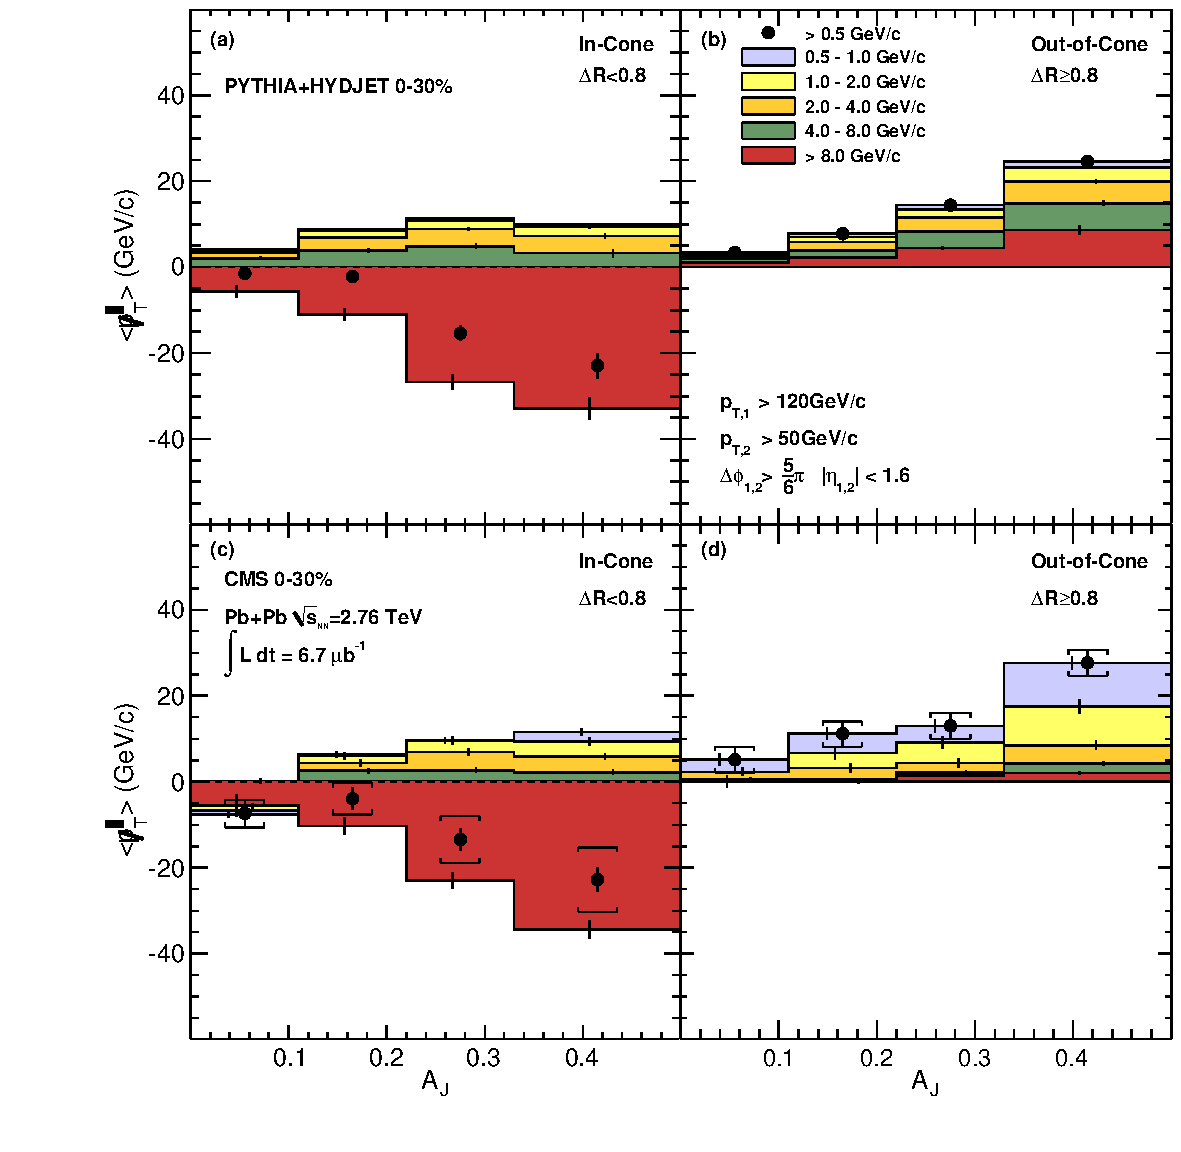
\includegraphics[width=0.7\textwidth]{jetfigures/missingPtParallel-Corrected-data-InConeOutConeDPhiCut_ntv6_2.pdf}
\caption{Average missing transverse momentum,
$\langle \displaystyle{\not} p_{\mathrm{T}}^{\parallel} \rangle$,
for tracks with $\pT > 0.5$\GeVc, projected onto the leading jet axis (solid circles).
The $\langle \displaystyle{\not} p_{\mathrm{T}}^{\parallel} \rangle$ values are
shown as a function of dijet asymmetry
$A_J$ for 0--30\% centrality, inside ($\Delta R < 0.8$) one of the leading or subleading jet cones (left) and
outside ($\Delta R > 0.8$) the leading and subleading jet cones (right).
For the solid circles, vertical bars and brackets represent
the statistical and systematic uncertainties, respectively.
For the individual $\pT$ ranges, the statistical uncertainties are shown as vertical bars.
Reproduced from~\cite{Chatrchyan:2011sx}.}
\label{fig:GR:CMS_missingpT}
\end{center}
\end{figure}

Focussing on asymmetric dijet events ($\AJ > 0.33$), both data and MC exhibit an
 in-cone imbalance of $\langle \displaystyle{\not} p_{\mathrm{T}}^{\parallel} \rangle \approx
-20$~\GeVc. This is balanced by an out-of-cone contribution of
$\langle \displaystyle{\not} p_{\mathrm{T}}^{\parallel} \rangle \approx 20$~\GeVc. The key
observation is that in the \PbPb\ data the out-of-cone contribution is found in the $0.5 < \pT < 4$~\GeVc\ region,
while in MC more than 50\% of the balance is carried at high $\pT > 4$~\GeVc. The MC
results can be interpreted as resulting from initial or final-state radiation (e.g.\ three-jet events).
For \PbPb\ events with large \AJ\ a large part of the momentum balance is
carried by soft particles ($\pT < 2$~\GeVc) at large angles to the jet axes ($\Delta R > 0.8$). This measurement
therefore has provided crucial information about the fundamental properties of the energy loss process
in the medium.

\subsection{Photon-jet correlations}

The use of the dijet and inclusive jet observables discussed in the previous sections
to extract information
about the absolute energy loss of the partons traversing the medium suffers from
uncertainties about the initial parton kinematics. E.g.\ for the dijet asymmetry
measurements in general both partons will suffer some amount of path-length dependent
energy loss, leading to ambiguities in the quantitative interpretation of the results
due to possible surface-biases.

These ambiguities can be largely overcome in studies of photon-jet events,
where the photon closely determines both the initial direction and momentum
of the back-to-back associated parton on an event-by-event basis.
Events where the photon and parton initial kinematics are most closely correlated
can be selected experimentally using an isolation requirement, which
increases the fraction of events with ``leading order'' prompt photons in
the photon-jet sample. The first measurement of isolated photon-jet correlations
was performed by CMS for a 150\mubinv \PbPb\ dataset~\cite{Chatrchyan:2012gt}.
To select ``isolated photons'', the energy in a cone around 
the photon candidate was required to be less than a threshold parameter~\cite{HIPhoton},
following a standard procedure developed for the analysis of \pp\ collisions. In the \PbPb\ 
environment, the isolation cut is applied after a subtraction of an event-by-event 
estimate of the underlying event contribution.

Following the approach for the study of dijet correlations, the photon-jet pairs
are characterized in terms of their azimuthal correlation, $\dphijg = |\phij - \phig|$,
 and momentum ratio, $\xjg = \ptj/\ptg$. In addition, the fraction of photons without
back-to-back jet partner,  \rjg, is studied, to provide information about
events where the jet lost sufficient energy to fall below the detection threshold.
For the CMS photon-jet analysis, photons were required to have $\ptg > 60\GeVc$
and  $|\eta^\gamma\|<1.44$. The associated jets were selected with
$\ptj > 30\GeVc$ and $|\eta^{\mbox{Jet}}|<1.6$. To study the correlations of
photons with their associated jets (rather than photon-inclusive jet or photon-leading
jet correlations), contributions from
coincidental photon-jet pairs were removed using a mixed event technique. In
addition, the contribution of background photons from e.g.\ hadron decays
were corrected using a data driven technique. The purity of the isolated photon-jet
sample was further enhanced by requiring $\dphijg > \frac{7}{8}\pi$.
Similar to the dijet correlations, no angular broadening
beyond the \pp\ data and MC reference was seen in the \PbPb\ data.

The photon-jet momentum correlations in \PbPb\ data were compared to a \PYTHYD\ reference
calculation as a function of collision centrality. The resulting
\xjg\ distributions are shown in Fig.~\ref{fig:GR:InclPtRatio_qcdPhoRef_pp2760-xJ30G60}.
Also shown is \avexjg\ distribution for 2.76\TeV\ \pp\ data, showing consistency
with the \PYTHYD\ calculation within the large statistical uncertainties.
The separate open and shaded red systematic uncertainty boxes illustrate the
anti-correlation of uncertainties across bins for the unity-normalized distributions.

\begin{figure}[!ht]
\begin{center}
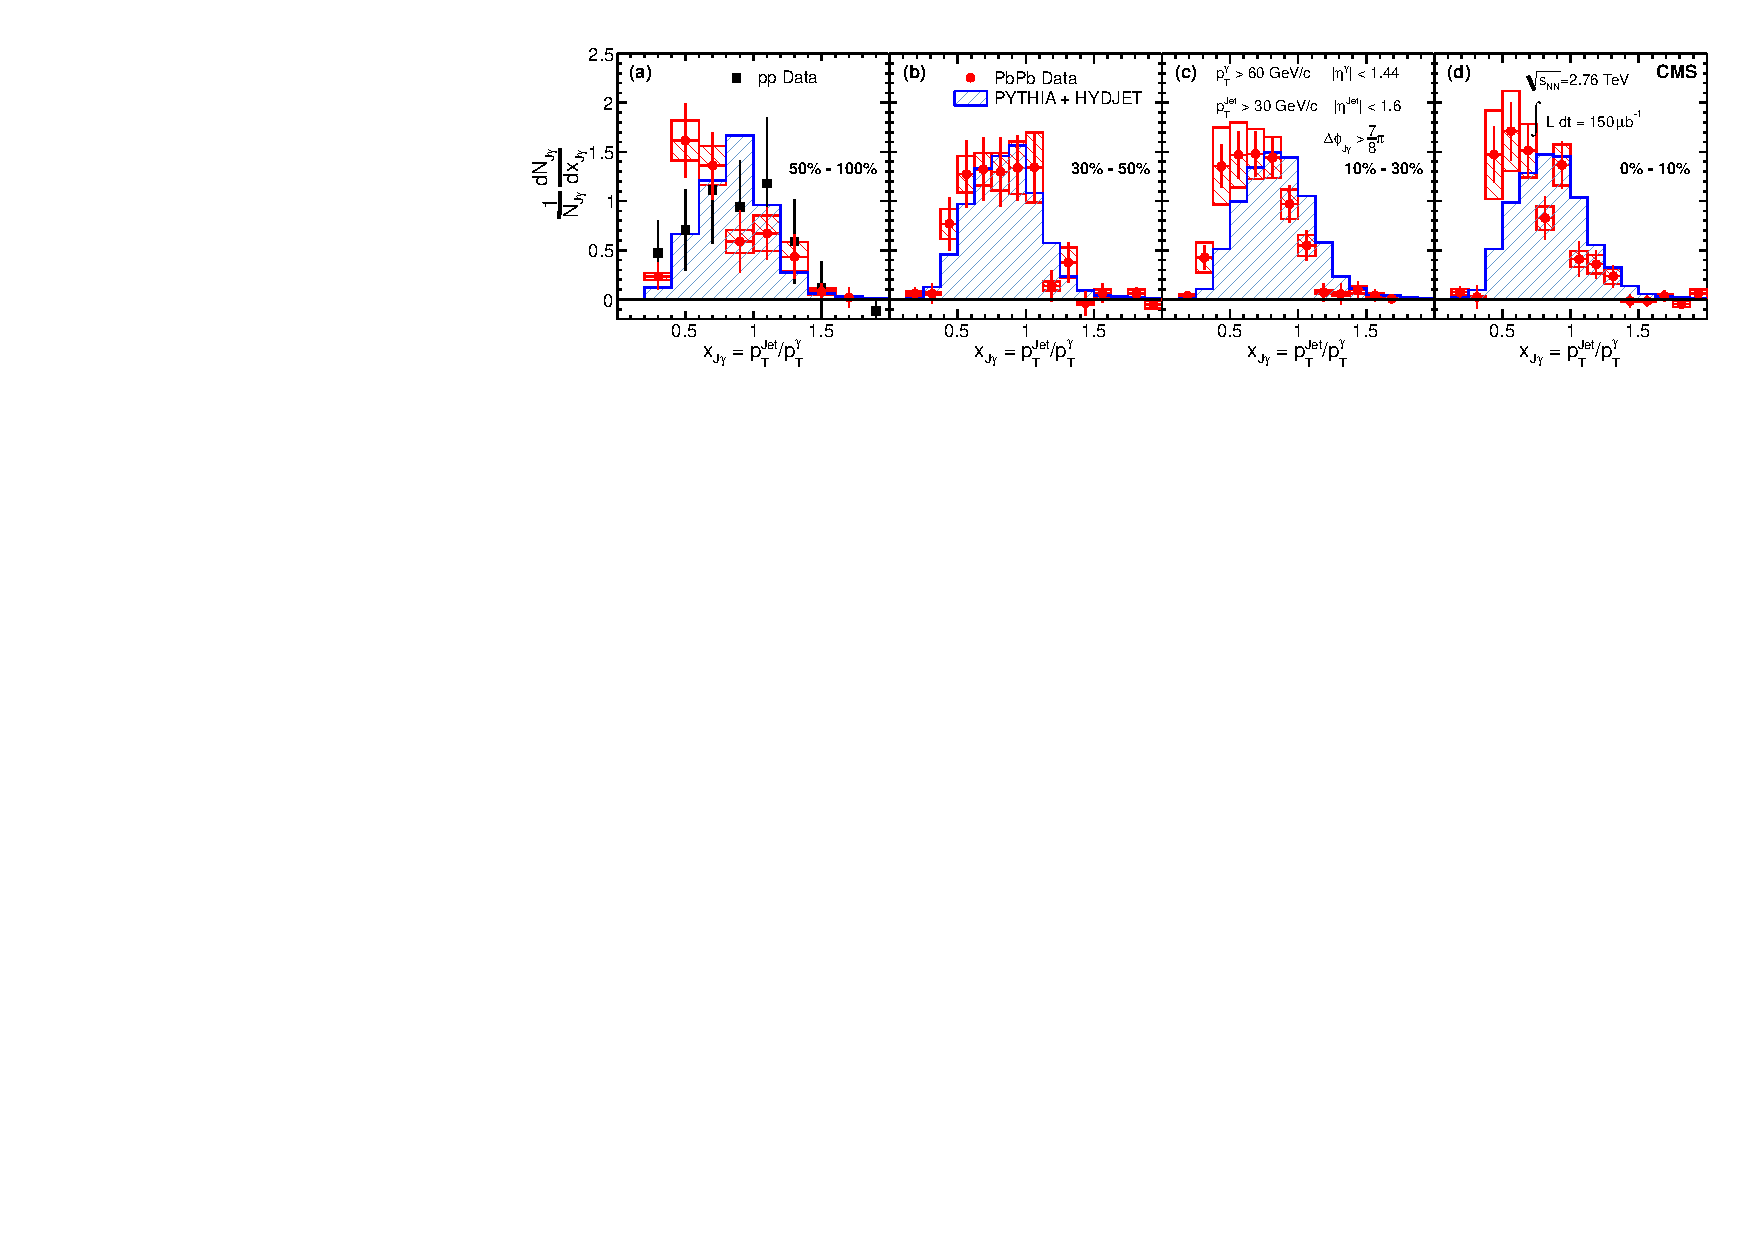
\includegraphics[width=0.98\textwidth]{jetfigures/Photonv7_Paper_InclPtRatio_all_cent4_G60J30_subDPhi1SS1_Isol0_Norm1log1.pdf}
\caption[]{\label{fig:GR:InclPtRatio_qcdPhoRef_pp2760-xJ30G60} Distribution of the photon/jet 
momentum ratio, \xjg, in four bins of collision centrality. 
  The distributions are normalised to unit area. All panels compare
\PbPb\ data (filled circles) to \pp\ data at
  2.76\TeV\ (filled squares), and to the \PYTHYD\ MC simulations
  (shaded histogram). Error bars show the statistical uncertainties and
boxes show the (anti-correlated) systematic uncertainties. Reproduced from~\cite{Chatrchyan:2012gt}.}
\label{fig:GR:CMS_xjg}
\end{center}
\end{figure}

For the most central events, the  photon-jet momentum balance  was found to be
$\avexjg_{0-10\%} = 0.73 \pm 0.02 \mbox{(stat.)} \pm 0.04 \mbox{(syst.)}$, compared
to a value of 0.86 predicted by \PYTHYD{} at the same centrality. This shift does
not include photon-jet events where the jet fell below the 30\GeV/c analysis threshold.
The \xjg\ observations are therefore complemented by studies of the fraction of
photons with a jet partner, \rjg.  The value of $\rjg$ decreases
from $\rjg = 0.685\pm 0.008\mbox{(stat.)}$--$0.698\pm 0.006\mbox{(stat.)}$ for \PYTHYD\
to  $\rjg = 0.49\pm 0.03\mbox{(stat.)}\pm 0.02\mbox{(syst.)}$--$0.54\pm 0.05\mbox{(stat.)}\pm 0.02\mbox{(syst.)}$ for
central \PbPb\ collisions. Combining these observations, the photon-jet studies
provide clear evidence of parton energy loss in the medium in events that are
largely free of surface and reconstruction biases for the jets. Future measurements
vs high statistics \pp\ reference data and with increased \PbPb\ statistics will
therefore allow a quantitative determination of the absolute parton energy loss
in the medium as a function of parton \pT.


\section{Heavy-flavour production}
\label{secks:heavy}
 Measurement of charm and beauty production plays a special role in heavy-ion physics: it provides a calibrated probe, as the input $p_{\rm T}$ spectra are calculable from perturbative QCD and measurable in pp collisions. In addition, this probe is conserved from its production at early stage of the collision until it escapes from interaction region, and is eventually detected. This enables a direct access to its interactions in the QGP, including the low- and intermediate-$p_{\rm T}$ regime. Two observables are studied:
 \begin{itemize}
 \item{transverse momentum dependence of the nuclear modification factor $R_{\rm AA}$ for charm and beauty paricles;}
 \item{azimuthal-flow anisotropy of charm and beauty particles, measured as the elliptic-flow coefficient $v_2$.}
 \end{itemize}
 These two topics are closely connected: the in-medium heavy-quark energy loss lowers the momenta of heavy quarks, they may then thermalize in the system, and thus participate in the collective-flow dynamics. The simultaneous measurement of the two quantities opens the possibility of the determination of the heavy-flavour transport coefficients.

 Two methods are exploited to detect heavy-flavour particles. Reconstruction of invariant mass of exclusive particle decays in a secondary vertex, displaced from the interaction one, is the primary tool. A second method uses the lepton ($\mu^\pm$ or e$^\pm$) $p_{\rm T}$ spectra to infer the heavy-flavour spectra, presuming that the leptons are produced in semi-leptonic decays of heavy-flavour particles. This way, however, a ($p_{\rm T}$-dependent) mixture of charm and beauty is measured. Sometimes a requirement that the lepton is not coming from the interaction vertex is used, which helps to eliminate the background, especially at lower $p_{\rm T}$ (below 4~GeV). The B-meson production is also accessible with the inclusive decay ${\rm B} \rightarrow {\rm J}/\psi + X$, using J/$\psi$ decays separated from the interaction point.
\subsection{Heavy-flavour spectra}
\label{subsecks:heavyspectra}
The $p_{\rm T}$ spectra of heavy-flavour particles are measured at the LHC in pp and Pb--Pb (and p--Pb) collisions. The pp results are compared to perturbative QCD calculations and other models~\cite{ALICE:2011aa,Abelev:2012vra}, giving information about preferred values for parameters, such as renormalization and factorization scales. The charm-particle spectra are measured down to very low $p_{\rm T}$ (down to 1~GeV in pp) allowing for precise determination of the total charm cross section at LHC energies. The pp spectra also serve as a normalization for Pb--Pb measurements~\cite{ALICE:2012ab}.

In general, the heavy-flavour spectra in heavy-ion collisions are expected to be also suppressed with respect to those in pp interactions, due to the energy quenching of heavy quark when traversing the dense medium. However, the energy loss of heavy quarks is predicted to be different than that of light quarks. For the energy loss by bremsstrahlung radiation, the quark energy loss will be mass dependent. The radiation is suppressed in directions close to that of the quark, for angles below $\Theta_0 \approx m/E = 1/\gamma$, due to a destructive interference ($m$, $E$, and $\gamma$ being the quark mass, energy, and gamma-factor, respectively). The heavier the quark, the larger the exclusion region (i.e. $\Theta_0$, at a given momentum), resulting in smaller energy loss for heavy quarks compared to the light ones. This is the so called dead-cone effect introduced for the vacuum radiation~\cite{Dokshitzer:1991fc} and later applied to the medium-induced radiation in a similar way~\cite{Dokshitzer:2001zm}. The predicted mass hierarchy is pronounced at $p_{\rm T}$ comparable with quark masses, and goes progressively away at very high $p_{\rm T}$. Recent model calculations include both the radiation and collisional energy loss, which results in larger suppression of heavy quarks, and gets values closer to the expectation for light ones.

There are other effects that modify the expected suppression pattern. At the LHC energies, the light-flavour particles at $p_{\rm T} \sim {\cal O}(10)$~GeV are mostly produced in gluon fragmentation, contrary to heavy-flavour ones produced by fragmentation of the corresponding heavy quarks. Gluons have larger colour charge than quarks by a factor 9/4, consequently a gluon has to suffer more energy loss than a quark. This colour-charge effect is reinforcing the expected difference in suppression between the light- and heavy-flavour particles. Further effects of less importance, taken into account in various models, are nuclear modification of structure functions and harder fragmentation function of heavy quarks compared to the light sector.

Charm mesons are identified in the following decay modes: ${\rm D}^0 \rightarrow {\rm K}^-\pi^+$, ${\rm D}^+ \rightarrow {\rm K}^-\pi^+\pi^+$, and ${\rm D}^{*+} \rightarrow {\rm D}^0\pi^+$ (and their antiparticles), requiring the decay vertex to be displaced from the interaction point. The yields of D mesons are corrected for the feed-down from beauty decays, obtained with model simulations. This contamination amounts to 5--15\,\% of the yields, depending on $p_{\rm T}$ and the particle type. The $p_{\rm T}$ spectra are measured both in pp~\cite{ALICE:2011aa,Abelev:2012vra} and Pb--Pb~\cite{ALICE:2012ab} collisions, and used to construct the nuclear modification factor $R_{\rm AA}$. The $p_{\rm T}$ dependencies of $R_{\rm AA}$ for three studied D-mesons are, as expected, compatible. Therefore, the results are combined into an average D-meson $R_{\rm AA}$ according their statistics, dominated by the ${\rm D}^0$. Figure~\ref{figks:DmesonRAA} compares the average D-meson $R_{\rm AA}$ as a function of $p_{\rm T}$ in central Pb--Pb collisions, with that of charged particles. The D-meson $R_{\rm AA}$ is perhaps a little bit above the charged-particle one, hinting at less suppression for charm quark, but the difference, if any, is very small. This tendency was recently confirmed with higher statistics charm measurements. The model calculations overlayed on data in Fig.~\ref{figks:DmesonRAA} are (I)~\cite{Sharma:2009hn,He:2011pd}, (II)~\cite{Horowitz:2011cv}, (III)~\cite{Horowitz:2011wm}, (IV)~\cite{Alberico:2011zy,Monteno:2011gq}, (V)~\cite{Gossiaux:2009mk,Gossiaux:2010yx}, (VI)~\cite{Fochler:2011en}, (VII)~\cite{Buzzatti:2011vt}, and (VIII)~\cite{Armesto:2005iq}. The various models show varying degrees of agreement with the charm results, and in general the inclusion of collisional energy loss improves the description. In model (I) the agreement is obtained by introducing in-medium dissociation of D mesons, in addition to radiative energy loss. The remaining models, which compute also the charge-particle $R_{\rm AA}$, have not reached good description for both cases, albeit some being not far.

\begin{figure}
\centering
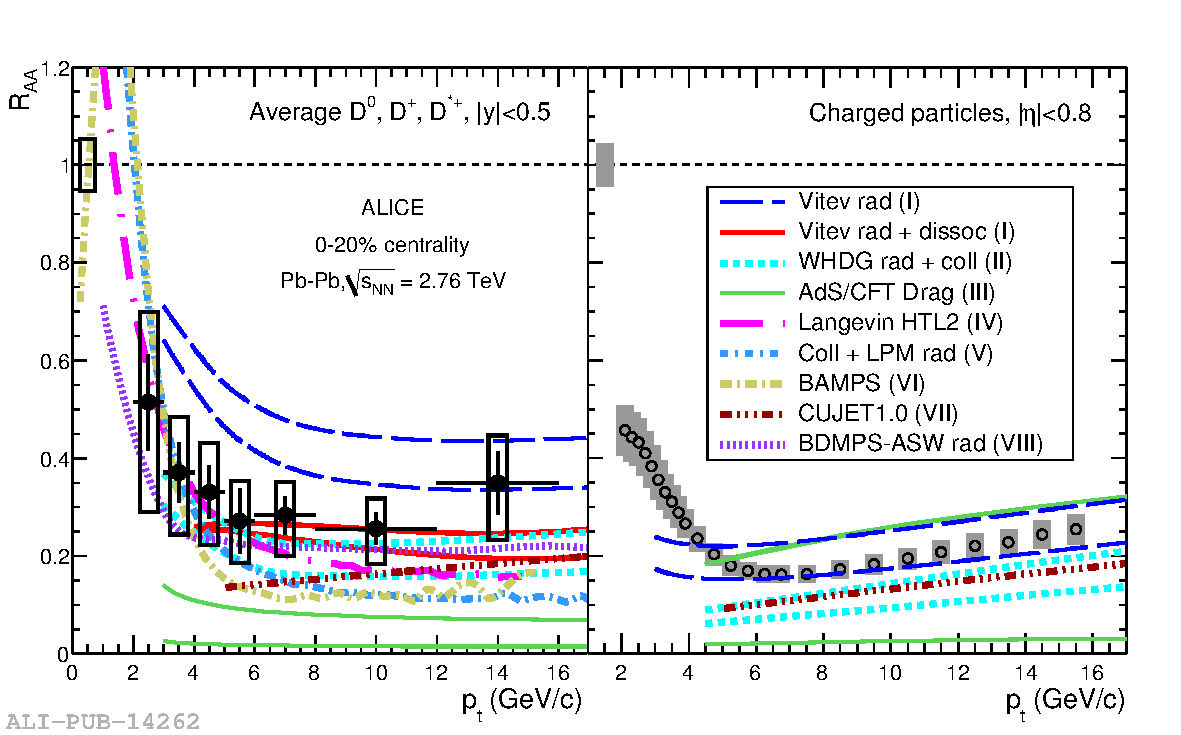
\includegraphics[width=0.7\textwidth]{ksfigures/DmesonChargedRAAmodels.pdf}
\caption{Average D-meson $R_{\rm AA}$ (left) and charged particle $R_{\rm AA}$ (right) as a function of $p_{\rm T}$ for the centrality between 0--20\,\%. The normalization uncertainties shown at unity in abscissa are almost fully correlated. The curves represent various model calculations, referred in the text, in some cases depicted as a range. Reproduced from~\cite{ALICE:2012ab}.}
\label{figks:DmesonRAA}
\end{figure}

Recently the family of measured D mesons was enlarged with the study of ${\rm D}_{\rm s}^+ \rightarrow {\rm K}^+{\rm K}^-\pi^+$ decay~\cite{Abelev:2012tca}. As a consequence of strangeness enhancement in heavy-ion collisions discussed in Sec.~\ref{subsecks:strangespectra}, the presence of strange quark may lead to a relative increase of ${\rm D}_{\rm s}$ production with respect to other D-mesons. Reported preliminary results show the ${\rm D}_{\rm s}$ $R_{\rm AA}$ in $p_{\rm T}$ region 4--12~GeV above the D-meson $R_{\rm AA}$, however, still within large uncertainties.

The behaviour of the charm-meson $R_{\rm AA}$ was confirmed by the measurement of the muon spectrum in the forward region $2.5 < y < 4$~\cite{Abelev:2012qh}. The contribution from pion and kaon decays is subtracted from the measured muon spectrum, and the results are presented for $p_{\rm T} > 4$~GeV, where this background contribution falls below 10\,\%. The obtained muon $p_{\rm T}$ spectrum thus represents a mixture of muons from semi-leptonic charm and beauty decays, presumably still dominated by charm at the lowest $p_{\rm T}$ and progressively becoming beauty dominated for $p_{\rm T} > 6$~GeV. An analogous  analysis of pp data is used for normalization, and the resulting heavy-flavour muon $R_{\rm AA}$ is presented in Fig.~\ref{figks:HFmuonRAA}. The muon $p_{\rm T}$, being correlated with the heavy-flavour-particle $p_{\rm T}$, is systematically smaller than the latter one (for $p_{\rm T}$ above a few GeV). Still, the comparison with the D-meson $R_{\rm AA}$ shows qualitative agreement, since the $p_{\rm T}$ dependence is rather flat. A similar measurement using electrons in mid-rapidity region was also reported~\cite{Abelev:2012xe}.

\begin{figure}
\centering
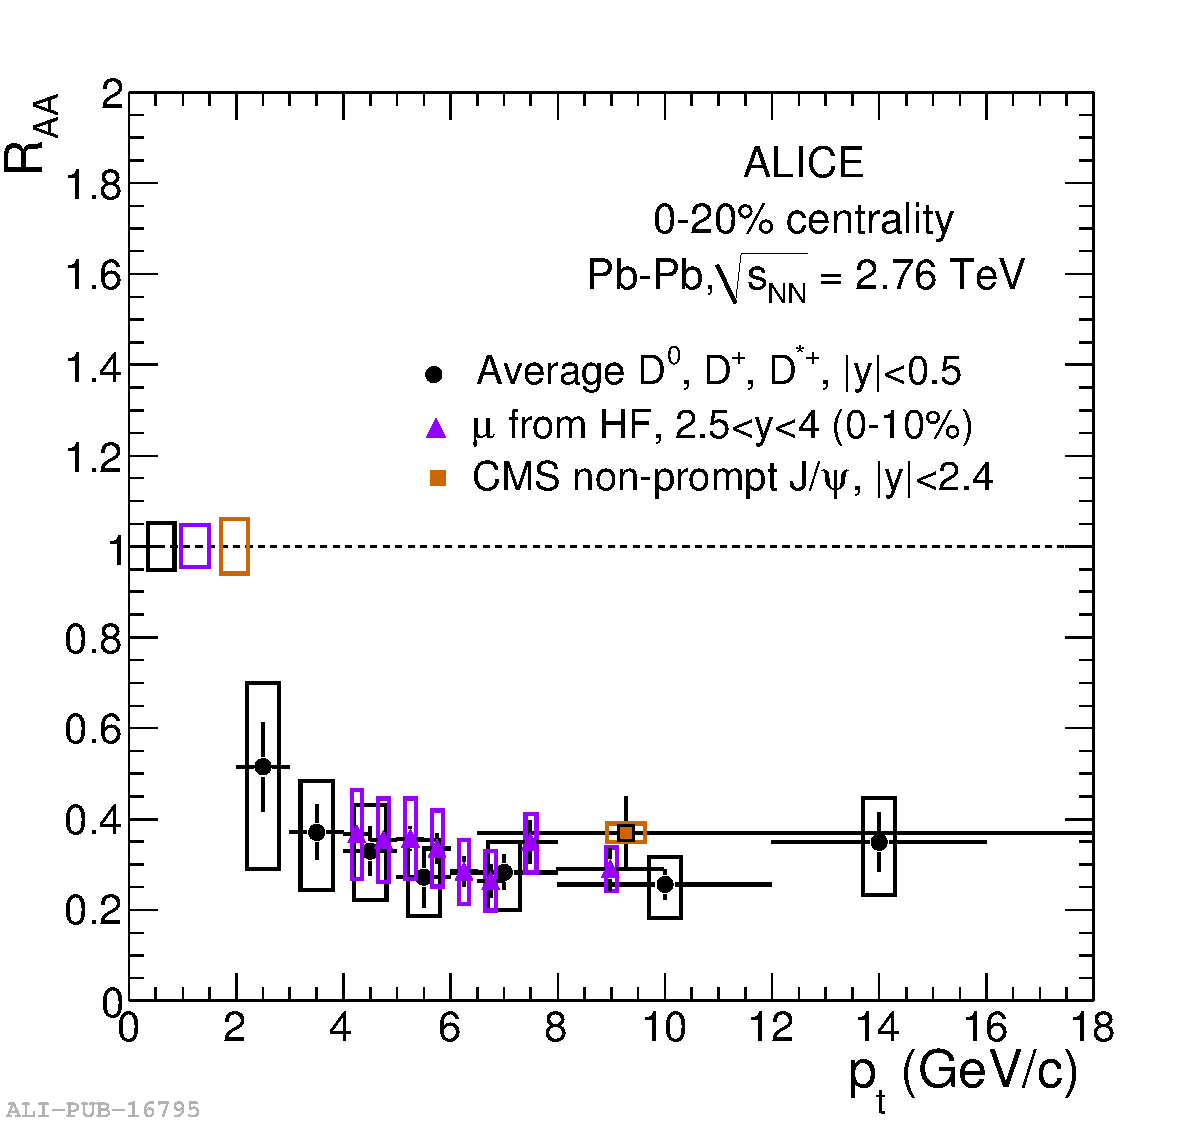
\includegraphics[width=0.5\textwidth]{ksfigures/DmesonHFmuonBRAA.pdf}
\caption{Heavy-flavour muon $R_{\rm AA}$ as a function of $p_{\rm T}$ compared to the average D-meson $R_{\rm AA}$. Results are for 0--20\,\% centrality class of Pb--Pb collisions. CMS preliminary result for beauty $R_{\rm AA}$ from measurement of non-prompt J/$\psi$ is shown with square. Reproduced from~\cite{Abelev:2012qh}.}
\label{figks:HFmuonRAA}
\end{figure}

In Fig.~\ref{figks:HFmuonRAA} the preliminary CMS result for $R_{\rm AA}$ from the measurement of non-prompt J/$\psi$ is shown~\cite{Chatrchyan:2012np}. The non-prompt J/$\psi$ particles are selected with careful analysis of the position of the J/$\psi$-decay point with respect to interaction vertex. These J/$\psi$'s are practically exclusively coming from B-meson decays. Recently reported detailed higher-statistics results on the centrality dependence of the $R_{\rm AA}$ for non-prompt J/$\psi$~\cite{CMS:2012wba} (in $p_{\rm T}$ range 6.5--30~GeV)  in comparison with the ALICE D-meson data (in $p_{\rm T}$ range 8--16~GeV) demonstrate clearly the larger $R_{\rm AA}$ for the beauty production than for the charm production, except for peripheral collisions, where the measurements are within their uncertainties. The shift between the $p_{\rm T}$ ranges takes into account that the J/$\psi$ momentum is lowered in the decay. This is for the first time that, as expected, the energy loss for beauty smaller than that for charm is experimentally observed.
%D-meson R_AA
%HF electron and muon R_AA
%Beauty suppression using B->J/psi+X
\subsection{Heavy-flavour elliptic flow}
\label{subsecks:heavyflow}
The primary cause of the elliptic azimuthal asymmetry is the asymmetric collision geometry: in semi-central collisions the overlapping region of the two nuclei has an almond shape, elongated in the direction perpendicular to the event plane (the plane defined by the beam axis and the centres of the colliding nuclei). The elliptic flow of charm was studied by the ALICE collaboration for D mesons using the event-plane method~\cite{Abelev:2013lca}. To estimate the azimuthal position of the event plane, charged tracks detected in the TPC are exploited. Then the yields of different D mesons are measured in the four azimuthal quadrants defined with respect to the event plane. From the yields in the two in-plane and in two out-of-plane quadrants the elliptic-flow coefficient $v_2$ is calculated. This is done independently for the three mesons: ${\rm D}^0$, ${\rm D}^+$, and ${\rm D}^{*+}$, and, as the $v_2$ values are compatible, they are then averaged applying beforehand the feed-down correction like in the case of the D-meson $R_{\rm AA}$. The $v_2$ results for the average D meson are presented in Fig.~\ref{figks:DmesonV2} for the centrality in the range 30--50\,\%. The comparison with the charged-particle $v_2$ obtained with the same method reveals a similar behaviour: the $v_2$ values for $p_{\rm T}$ between 2--8~GeV are compatible. This is the first direct observation of non-zero $v_2$ for a heavy-flavour particle. The large value of the charm $v_2$ at $p_{\rm T}$ around 2~GeV is interpreted as a signature of the in-medium thermalization of charm quarks.

\begin{figure}
\centering
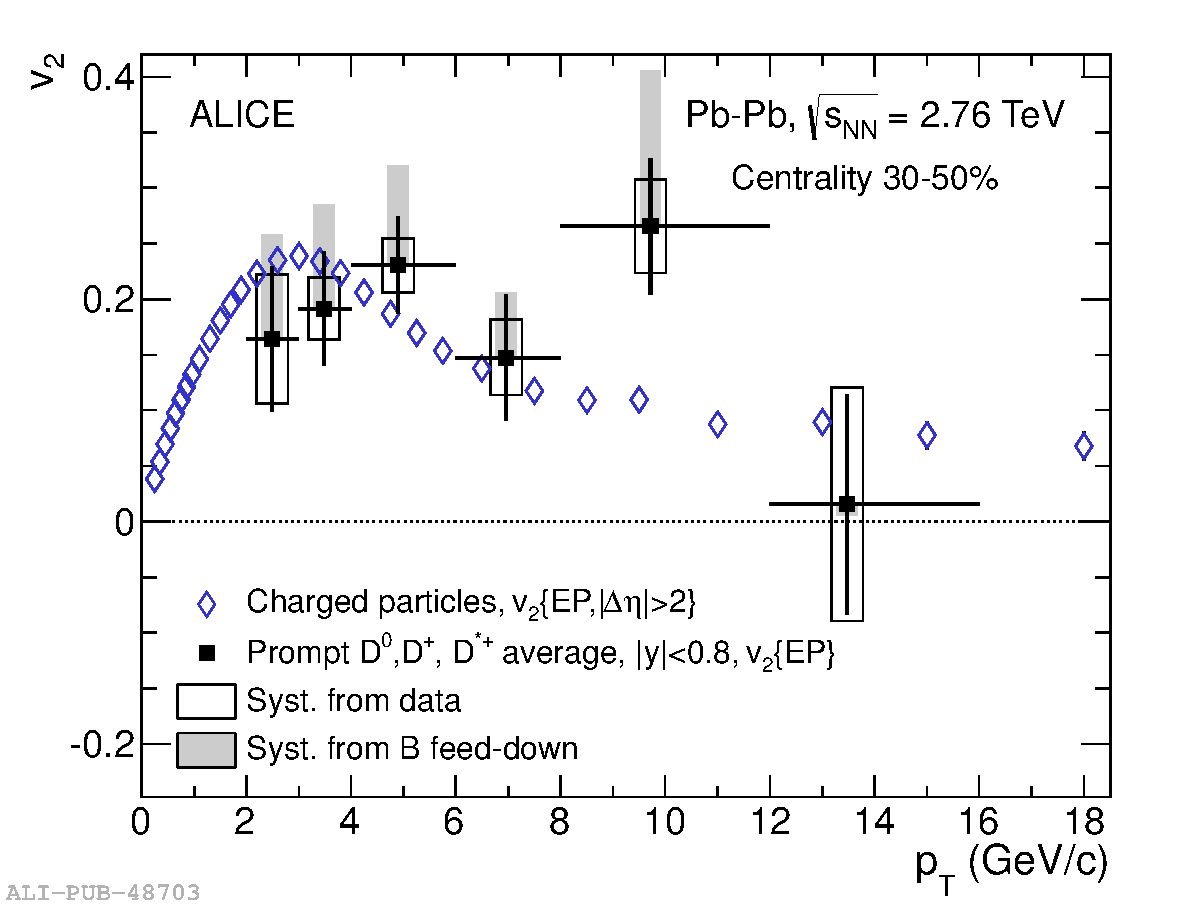
\includegraphics[width=0.5\textwidth]{ksfigures/DmesonV2.pdf}
\caption{Elliptic-flow coefficient $v_2$ obtained with the event-plane method, as a function of $p_{\rm T}$ for the centrality 30--50\,\%, averaged for ${\rm D}^0$, ${\rm D}^+$, and ${\rm D}^{*+}$, compared to the charged-particle measurement. Reproduced from~\cite{Abelev:2013lca}.}
\label{figks:DmesonV2}
\end{figure}

At higher $p_{\rm T}$ a positive $v_2$ can be generated by the difference in the in-medium path lengths for charm quarks emitted inside the in-plane azimuthal quadrants compared to those emitted in the out-of-plane quadrants. The shorter path length for the in-plane partons implies less suppression, i.e. larger $R_{\rm AA}$ for particles produced in this direction, than for those produced in the out-of-plane direction. In fact, the results can be presented as an azimuthally-dependent $R_{\rm AA}$, which is equivalent to the azimuthally-integrated $R_{\rm AA}$ and the $v_2$. The interpretation of the high-$p_{\rm T}$ $v_2$ as a path-length effect opens the possibility of studying  the in-medium path-length dependence of the parton energy loss.

The $v_2$ results for D mesons are complemented by the recently reported elliptic-flow measurements at forward rapidities ($2.5 < y < 4$) for the muons from heavy-flavour decays. They show an effect of similar magnitude. Indication of non-zero heavy-flavour $v_2$ using the semi-leptonic decays were previously published by RHIC experiments~\cite{Adler:2005ab,Adare:2006nq}.
%D-meson v2
%HF lepton v2

\section{Quarkonium production}
\label{sec:qurkonia}
Measurements of quarkonium production promise to yield important information about the
strongly-interacting system formed in heavy-ion collisions.  The in-medium dissociation of quarkonium states
in these collisions is expect to reflect both the states binding energy as
well as the temperature of the medium, leading to a sequential suppression or disappearance
of the various charmonium and bottomonium states~\cite{Matsui:1986dk,Digal:2001ue}.

\jpsi\ production in heavy-ion collisions has been studied over a wide range of
collisions energies at the CERN SPS and RHIC, with a strong suppression of \jpsi\
yields observed in central collisions for $\rootsNN \approx 20$ to
$200$~GeV~\cite{Alessandro:2004ap,Adare:2006ns,Adare:2011yf}.
The interpretation of the observed suppression is complicated by the presence
of Cold Nuclear Matter effects such as nuclear absorption and (anti-) shadowing. A quantitative
description furthermore needs to take into account feeddown from excited states,
which contribute a significant fraction of the inclusive \jpsi\ yield in \pp collisions.
Finally, and perhaps most importantly, the large abundance of deconfined charm quarks
at RHIC and higher energies requires the consideration of a recombination component
in addition to direct \jpsi\ production, which may mask the suppression of the initial
\jpsi\ formation~\cite{BraunMunzinger:2000px,Thews:2000rj,Andronic:2007bi,Zhao:2007hh}.

The large increase in the charm cross-section at LHC should magnify these regeneration
effects compared to lower energy collisions, and thus provide the opportunity to disentangle
suppression and regeneration effects in a study of the collision energy,
\pT\ and rapidity dependence of \jpsi\ production.

The LHC collision energies also facilitate high statistics studies of the \PgU\ family, where
the three \PgUn\ states are connected by the common initial bottom pair production and
similar kinematics, but distinguished by the hierarchy of their binding energies. In an
in-medium dissociation picture, one therefore expects a distinct pattern in the suppression
of the \PgUn\ states.

\subsection{Charmonium suppression}

J/$\psi$ production in \PbPb\ collisions can be characterized relative to the \Ncoll-scaled \pp\ reference
distributions, using the \Rcp\ and \Raa\ nuclear modification factors introduced earlier.
A strong suppression of high-\pT\ inclusive \jpsi\ in the dimuon decay channel was observed in central \PbPb\ collisions
at $\rootsNN = 2.76$ TeV  relative to peripheral \PbPb\ collisions by ATLAS~\cite{Aad:2010aa}
and with respect to \pp\ collisions by CMS~\cite{Chatrchyan:2012np}.

Results for the suppression of low \pT\ \jpsi\ production from ALICE~\cite{Abelev:2012rv} are shown
in Fig.~\ref{fig:GR:raavsy} for $\pT > 0$\GeVc\ (square markers) and
$\pT > 3$\GeVc\ (diamond markers), together with CMS data~\cite{Chatrchyan:2012np}
for rapdity $ 1.6 < |y| < 2.4 $ and $\pT > 3$\GeVc (triangle markers).

\begin{figure}
\begin{center}
\includegraphics[width=0.49\linewidth]{qqbarfigures/RAAvsY_v7-eps-converted-to.pdf}
\caption{ \label{fig:GR:raavsy}  Inclusive \jpsi\ \Raa\ measured in \PbPb\
collisions at $\rootsNN = 2.76$\TeV\ as a function of  rapidity for two \pT\ ranges.
Total systematic uncertainties are displayed as open boxes, not including
uncertainties on the \pp\ luminosity and \Taa\ scaling factor.  These are
5.2\% and  8.3\% for ALICE and CMS, respectively.
Two model predictions are shown~\cite{Ferreiro:2011rw,Vogt:2010aa} including only shadowing effects
for  nDSg (shaded areas) and EPS09 (lines) nPDFs. Reproduced from~\cite{Abelev:2012rv}.}
\end{center}
\end{figure}

Within uncertainties, neither \pT\ range shows a strong dependence of \jpsi\ suppression on rapidity.
The suppression is stronger than predicted for shadowing effects in the Color Singlet
Model~\cite{Ferreiro:2011rw} and the Color Evaporation Model~\cite{Vogt:2010aa}. Neither model
predicts a strong rapidity dependence.

A stronger initial state suppression has been seen in the Color Glass Condensate (CGC) model~\cite{Dominguez:2011cy},
predicting  \jpsi\ $\Raa \approx 0.5$. This prediction can be confronted with the \pT\ dependence
of \jpsi\ suppression, where initial state suppression models typically lead
to a stronger suppression at lower \pT.
In contrast, possible \jpsi\ regeneration effects in statistical hadronization~\cite{{BraunMunzinger:2000px, Thews:2000rj}}
or partonic transport~\cite{{Zhao:2007hh},{Liu:2009nb}} models are expected to enhance
\jpsi\ yields at low \pT\ due to the higher phase space density of charm quarks at lower \pT.

Data from ALICE and CMS on the \pT\ dependence of the \jpsi\ \Raa\ integrated over a wide range of \PbPb\ collision centrality
are shown in Fig.~\ref{fig:GR:raaexp2}. Although the measurements
cover different rapidity ranges ($2.0 < |\y| < 4.0$ vs $ 1.6  < |\y| < 2.4 $)
a common, strong \pT\ evolution of \jpsi\ \Raa\ is seen, ranging from $\approx 0.8$ at low \pT\ to $\approx 0.4$ for $\pT > 5$\GeVc.
This observation clearly favors models including a low-\pT\ enhancement due to charm recombination.

An even more striking observation is shown in the bottom panel of Fig.~\ref{fig:GR:raaexp2}, which compares
the ALICE forward-rapidity \jpsi\ \Raa\ for 0\%--20\% central \PbPb\ collisions at  
$\rootsNN = 2.76$\TeV~\cite{Abelev:2013ila}
with central \AuAu\ data from PHENIX at $\rootsNN = 0.2$\GeV and rapidity $1.2 < |\y| < 2.2$~\cite{Adare:2011yf}.
At low \pT\ the ALICE \Raa\ is about four times larger than that seen at the lower energy, while
at the same time the initial energy density of the system at LHC is estimated to be larger than at
RHIC by a similar factor. While a quantative interpretation of this result will require
a detailed understanding of CNM effects at the two energies, the results are qualitatively consistent
with the collision energy trend expected in recombination approaches such as~\cite{Zhao:2007hh,Zhou:2013aea,Liu:2009nb}.
First results of \jpsi\ production in \pPb\ collisions at the LHC have recently
been presented~\cite{Abelev:2013yxa,Aaij:2013zxa}, allowing
the calibration of CNM effects vs final state suppression and recombination.

\begin{figure}[h!]
\begin{center}
\includegraphics[width=0.49\linewidth,keepaspectratio]{qqbarfigures/RAAPtvsModels1.pdf}
\includegraphics[width=0.49\linewidth,keepaspectratio]{qqbarfigures/RAAPtvsModels2.pdf}
\caption{ \label{fig:GR:raaexp2}
(Top): \pT\ dependence of \jpsi\ \Raa\ measured by ALICE in \PbPb\
collisions (0--80\% centrality) at $\rootsNN = 2.76$\TeV compared to CMS~\cite{Chatrchyan:2012np}
results (0--100\% centrality) at the same energy.
(Bottom): \pT\ dependence of the \jpsi\ \Raa\ measured by ALICE in the 0\%--20\% most
central \PbPb\ collisions at 2.76\TeV\ compared to PHENIX~\cite{Adare:2011yf}
results in the 0\%--20\% most central \AuAu\ collisions at 200\GeV. Reproduced from~\cite{Abelev:2013ila}}
\end{center}
\end{figure}


\subsection{Charmonium elliptic flow}

An important question for models implementing the competing contributions of
\jpsi\ dissociation in the medium and \jpsi\ regeneration via charm quark recombination is
the degree of charm quark thermalization. The question of thermalization in heavy-ion collisions is typically addressed
via studies of hydrodynamic flow. ALICE has recently presented the first data suggesting non-zero elliptic flow
in \PbPb\ collisions, providing important information on this topic.

In a dissociation/recombination type approach, elliptic flow of the observed \jpsi\ can arise from multiple
contributions. Those \jpsi\ produced in the initial hard scattering traverse a shorter path in the medium when
travelling in-plane vs out-of-plane, leading to a possible azimuthal modulation of \jpsi\ yields with respect
to the event plane. If charm quarks participate in the collective expansion of the medium, as
suggested by the observed elliptic flow of open charm mesons, \jpsi's produced by recombination will
pick up the elliptic flow of the charm quarks. These contributions can possibly be disentangled by
studies of the \pT\ dependence of \jpsi\ suppression and \jpsi\ elliptic flow.

Measurements of the \jpsi\ elliptic flow by STAR for \AuAu\ collisions at $\rootsNN = 200$\GeV
are consistent with zero~\cite{Adamczyk:2012pw}, altough the large uncertainties prevent strong conclusions.
\begin{figure}
\begin{center}
\includegraphics[width=0.49\linewidth]{qqbarfigures/prl_fig4-eps-converted-to.pdf}
\caption{\label{fig:GR:v2ptcomp} Inclusive \jpsi\ \vtwo\
for \PbPb\ collisions with 20--60\% centrality at $\rootsNN = 2.76$\TeV\ as a function of \pT.
Also shown are calculations from two transport models~\cite{Liu:2009gx,Zhao:2012gc}. 
Reproduced from~\cite{ALICE:2013xna}}
\end{center}
\end{figure}
The ALICE measurement of \jpsi\ \vtwo\ as a function of transverse momentum is shown in Fig.~\ref{fig:GR:v2ptcomp} for \PbPb\ collisions
in the 20\%--60\% centrality range~\cite{ALICE:2013xna}.
The \jpsi\ \vtwo\ data, which have a significance of about 2$\sigma$ in this centrality range, are compared to two
transport model calculations~\cite{Liu:2009gx,Zhao:2012gc}. The models, which include charm quark recombination effects,
are both compatible with the data within the current large experimental uncertainties. The comparison points to the
importance of future high statistics measurements of \jpsi\ elliptic flow at high transverse momentum ($\pT > 5$\GeVc).

In combination, the \pT\ and collision energy dependence of \jpsi \Raa\ and the indication of non-zero \jpsi\ elliptic
flow suggest a possible  contribution of charm quark recombination to \jpsi\ production in \PbPb\ collisions
at LHC.

\subsection{Upsilon suppression}

Measurements by CMS have provided the first high statistics look at \PgU\
production in heavy-ion collisions~\cite{CMS_Y_2010}.
The \PgU\ family, with similar decay kinematics but a large variation of binding energies,
provides an ideal laboratory to test dissociation effects in the hot medium produced in
heavy-ion collisions. Compared to charmonium suppression studies, uncertainties due
to CNM effects and feed-down from higher mass states are expected to be
less important for the bottomonium family.

Dimuon invariant mass spectra in the \PgU\ mass range obtained by CMS are shown in Fig.~\ref{fig:GR:mass} for \PbPb\ (left)
and \pp\ (right)~\cite{Chatrchyan:2012lxa}. The data correspond to integrated luminosities of $150\mubinv$ and $230 \nbinv$ for
\PbPb\ and \pp, respectively. For the \pp\ data, the excellent mass resolution of the CMS muon system
allows a clear separation of the three \PgUn\ states. A similar mass resolution is achieved for \PbPb\ collisions.
However, for \PbPb\ a strong suppression of the \PgUb\ state is evident from the distribution, and the \PgUc\ state
is no longer visible above the continuum background. This is a striking visual confirmation of the expected
\PgU\ suppression pattern as a function of the \PgUn\ binding energy, and confirmed the first \PgU\ measurements
reported in~\cite{CMS_Y_2010}.

\begin{figure}[t]
\begin{center}
    \includegraphics[width=0.45\textwidth]{qqbarfigures/hiFitPt4Erf}
    \includegraphics[width=0.45\textwidth]{qqbarfigures/ppFitPt4Erf}
    \caption{Dimuon invariant-mass distributions in \PbPb\ (left) and \pp\ (right)
at $\rootsNN = 2.76$\TeV. \PbPb\ and \pp\ were reconstructed with identical
reconstruction algorithms and analysis selections. The lines show simulataneous fits to both
datasets for signal + background (solid) and background-only (dashed).
Reproduced from~\cite{Chatrchyan:2012lxa}}
\label{fig:GR:mass}
\end{center}
\end{figure}

The comparison of \pp\ and \PbPb\ data allows a characterization of the \PgU\ suppression
in terms of the nuclear modification factor \Raa.
Integrating over centrality, the following \Raa\ values were measured for the \PgUn states:
\begin{eqnarray}
\Raa (\PgUa) &=& 0.56 \pm 0.08\,\text{(stat.)} \pm 0.07\,\text{(syst.)} \,, \\
\Raa (\PgUb) &=& 0.12 \pm 0.04\,\text{(stat.)} \pm 0.02\,\text{(syst.)} \,, \nonumber \\
\Raa (\PgUc) &=& 0.03 \pm 0.04\,\text{(stat.)} \pm 0.01\,\text{(syst.)} .  \nonumber
\end{eqnarray}
The statistical significance of the \PgUc\ peak above the continuum is less than one standard deviation.
It should also be noted that there are significant feed-down contributions to
the \PgUa\ state that may reach $\approx 50\%$~\cite{Affolder:1999wm, Aaij:2012se}.
This could mean that directly produced \PgUa\ state are largely unsuppressed, with
the observed \PgUa\ \Raa\ of 0.56 reflecting the dissociation of the higher mass excited states.

The \PgUa\ and \PgUb\ suppression was also studied as a function of centrality,
as shown in Fig.~\ref{fig:GR:centrality}.
Here the relative suppression of \PgUa\ and \PgUb\ is characterized by
the double ratio \linebreak $({\PgUb/\PgUa})_{\rm PbPb}/({\PgUb/\PgUa})_{\rm pp}$
(Fig.~\ref{fig:GR:centrality}~(left) and the absolute suppression
of the two states is shown as \Raa\ vs centrality (Fig.~\ref{fig:GR:centrality}~(right)).

\begin{figure}[t]
\begin{center}
   \includegraphics[width=0.45\textwidth]{qqbarfigures/chi2VsCent}
   \includegraphics[width=0.45\textwidth]{qqbarfigures/RaaPt4}
  \caption{(Left): Centrality dependence of the \PgUa\ and \PgUb\ double ratios
for 2.76\TeV\ \PbPb\ collisions.  (Right):
Centrality dependence of \Raa\ for $\PgUa$ and $\PgUb$ for 2.76\TeV\ \PbPb\ collisions.
Error bars show statistical uncertainties, while the boxes around the points
show systematic uncertainties. Common, \npart-independent
uncertainties are represented by the boxes at unity. Reproduced from~\cite{Chatrchyan:2012lxa}}.
\label{fig:GR:centrality}
\end{center}
\end{figure}

While \Raa\ shows a strongly falling trend with increasing collision centrality
for both \PgUa\ and \PgUb\ (with a much stronger suppression for \PgUb), the
double ratio does not exhibit a pronounced centrality dependence.

Overall, the data qualitatively exhibit the hierarchy in the \PgUn\ suppression pattern
expected based on the states' binding energies. Although the most peripheral bin
is rather wide (50--100\%), it is interesting to observe the strong suppression of the
\PgUb\ relative to the \PgUa\ already for this bin. Future high statistics \PbPb\ data
should elucidate the onset of the \PgU\ suppression in the most peripheral collisions,
in combination with information on \PgU\ suppression in small systems obtained from
studies in \pPb\ reference data.


\section{Summary and outlook}
\label{secall:summary}
This review has attempted to summarize the broad range of new data from the first two
runs with lead ions in collision at the CERN Large Hadron Collider.
To date, about 150~$\mu$b$^{-1}$ of data have been collected by each of
three major LHC experiments (ALICE, ATLAS and CMS), corresponding to about three billion
minimum-bias events sampled between them.
The three detectors are all large, multi-purpose spectrometers, with ALICE being optimized
for particle identification at low $p_{\rm T}$, photons, and muons at forward rapidity;
ATLAS and CMS optimized for precision measurements
of high \pT\ objects (tracks, jets, muons, electrons and photons).
The centrality of the collision is estimated in all of the experiments by partitioning
the event distribution of the forward transverse energy or multiplicity into
intervals corresponding to percentiles of the collected events, and related to
the nuclear overlap geometry using Glauber models.
Good agreement in the centrality estimation is found between the experiments, as illustrated
by the charged particle multiplicity per participant pair, as a function of centrality.
The centrality is also crucial for measuring the suppression of high \pT hadrons, relative
to what is measured in proton-proton collisions, via the ratio $R_{\mathrm{AA}}( \pT )$.
The value of $R_{\mathrm{AA}}$ is found to be strongly suppressed at low \pT, but then to rise
and plateau again at a level of about 0.5, similar to what is found for jet suppression.
The detailed study of identified particle yields shows good consistency with thermal models,
except for an anomalous suppression of protons.
Just as it was at the CERN SPS and RHIC, the yield of strange hadrons, and especially multi-strange, is substantially
enhanced in heavy-ion collisions.
Two particle correlations provide a rich handle on soft physics in heavy ions, giving
insight into the space--time structure (via HBT measurements), jets, and the so-called
``ridge''.  Despite not being a full jet measurement, correlations provide similar insight
into the suppression of the away-side region and an enhancement on the near-side
suggestive of modified jet fragmentation in medium.
The geometric dependence of charge fluctuations and the charged balance function provide
information on the fate of conserved quantities in the medium evolution.
Finally, more sophisticated correlations meant to look for the Chiral Magnetic Effect (CME)
find consistency with STAR data from RHIC, but no clear indication of the CME.

Collective flow has been extensively measured at the LHC by all the experiments.
Both two-particle and multi-particle methods have been used, which have varying sensitivity to
the presence of non-flow effects, such as correlations from jet production and fragmentation.
Various scaling behaviors have been observed, both for the absolute value of $v_2$ (even at
large \pT), as well as $v_2$ scaled by the overlap eccentricity.
The LHC has also seen an explosion in the measurement of higher-order harmonics up to $v_6$,
and the rapidity-even and -odd contributions to $v_1$, all of which should
allow more stringent tests of hydrodynamic models.
Event-by-event flow fluctuations have also been measured both by unfolding reconstructed
distributions as well as by using combinations of cumulants.  Good consistency has been found
for $v_2$ fluctuations over a wide range of centrality, while differences in $v_3$
fluctuations may be attributable to the different methods used to extract it.

Hard processes have been well calibrated using measurements of electro-weak bosons: both
W and Z as well as photons.  All of these particles are found to have cross sections
(both total and differential)
consistent with perturbative QCD calculations scaled by the number of binary collisions.
No substantial modifications of the nuclear parton distributions functions appears to be needed, due to the good
agreement of rapidity-dependent quantities.
In this context, the modifications of jets in more central heavy ion collisions can more
clearly be attributed to the energy loss of partons traversing the hot, dense medium.
Energy loss has been addressed using several techniques, from dijet imbalance
to single jet suppression, both inclusive and differentially in $\varphi$.  Jet fragmentation and
jet shapes in heavy-ion collisions have also been measured and found to be modified, with
studies of the overall energy flow in dijet events recovering the ``missing'' energy in
the jet cone at large angles with respect to the jet axis.
Correlations of jets with photons shows a similar energy loss effect, using a process that allows
tagging of the initial hardness scale.

Heavy flavor is produced copiously at the LHC and is expected to show different energy loss than
light quarks.  Early results show strong suppression of D mesons as well as J$/\Psi$ from
B-meson decays, as well as a significant signal that D mesons participate in the collective flow.
Quarkonia (both J$/\psi$ and $\Upsilon$ states) have also been studied over a wide range of \pT\
and rapidity.  The J$/\psi$ yield is found to be suppressed at a similar level over a wide
rapidity range, although the suppression at low $\pT$ is not as strong as it was at
RHIC, suggesting the possibility of regeneration processes due to the large charm quark production
rates.  Similar to what was found for open charm, the forward J$/\psi$ have a
$2\sigma$ significant $v_2$ signal, potentially larger than was found at RHIC.
The $\Upsilon$ family show interesting behavior in heavy ion collisions, with all states being
suppressed relative to proton-proton collisions, and the more weakly bound higher states showing
stronger suppression than the more tightly bound 1S state.

The results shown here are mainly the ones submitted to journals for publication, and many more
results are in preparation.  Thus, this review should be seen mainly as a snapshot of
the state of the field.  The wealth of upcoming results from the first two lead--lead runs,
and the upcoming runs with higher energy ($\energy = 5.5$ TeV) and luminosity
exceeding the design instantaneous luminosity of $10^{27}$~cm$^{-2}$s$^{-1}$ should
provide even further insight into
the nature and properties of the hot, dense matter formed in nuclear collisions at the LHC.

The progress towards a detailed characterization of this strongly
interacting state of matter will generally focus more on rarer probes,
and the study of their coupling with the medium and
hadronization. These will include heavy-flavour particles, quarkonia
states, real and virtual photons, jets and their correlations with
other probes (particularly photons and electroweak bosons).  The cross
sections of all these processes are significantly larger at LHC than
at previous accelerators. In addition, the interaction with the medium
of such hard probes is better controlled theoretically than the
propagation of soft light partons.

To achieve these goals high integrated luminosities and high precision measurements
are required, which will give access to the rare physics channels
needed to understand the dynamics of this condensed phase of QCD.
Therefore, the LHC collaborations are upgrading the current
detectors to enhance their vertexing capability, and allowing data
taking at substantially higher rates.  The upgrade strategy for
heavy-ion running is formulated under the assumption that, after the
second long shutdown in 2018, the LHC will progressively increase its
luminosity with Pb beams eventually reaching an interaction rate of
about 50~kHz, i.e. instantaneous luminosities $6 \times
10^{27}$~cm$^{-2}$s$^{-1}$. The proposed plan~\cite{ALICEUpgradeLoI}
envisages to accumulate 10~nb$^{-1}$ of Pb--Pb collisions inspecting
${\cal O}(10^{10})$ interactions, which is needed to address the
proposed physics programme, with focus on rare probes both at low- and
high-transverse momenta as well as on the multi-dimensional analysis
of such probes with respect to centrality, event plane, and
multi-particle correlations.


\bibliography{heavyion}

\end{document}

